\documentclass[a4paper,10pt,openany]{book}
\usepackage{fullpage}
\usepackage{ifxetex}

\ifxetex
    \usepackage{fontspec}
    \setmainfont[Mapping=tex-text]{TeX Gyre Pagella} % Pallazo
    \usepackage{graphicx}
\else
    \usepackage[utf8]{inputenc}
    \usepackage{ucs}
    \usepackage[T1]{fontenc}
    \usepackage{tgpagella}
    \usepackage{graphicx}
\fi

\DeclareGraphicsExtensions{.pdf,.eps,.png,.jpg}

\usepackage[brazilian]{babel}
\usepackage{url,color,float}
\usepackage{multirow}
\usepackage{indentfirst}
\usepackage{multicol}
\usepackage{fancyhdr}
\usepackage{dblfloatfix}
\usepackage{fixltx2e}
\usepackage{wrapfig}
\usepackage{enumitem}
\usepackage{hyperref}
\hypersetup{
    bookmarks=true,
    pdftitle={Manual do Bixo \the\year},
    pdfauthor={Centro Acadêmico da Computação - CACo},
    hidelinks
}


%%%%% Headers and Footers
\pagestyle{fancy}
\fancyhf{}
\fancyhead[LE, RO]{Manual do Bixo \the\year}
\fancyhead[RE]{\rightmark}
\fancyhead[LO]{\leftmark}
\fancyfoot[EL, OR]{\thepage}
\fancyfoot[RE]{Centro Acadêmico da Computação}
\fancyfoot[LO]{CACo}
\renewcommand{\headrulewidth}{0.2pt}
\renewcommand{\footrulewidth}{0.2pt}
\renewcommand{\headsep}{15pt}
\renewcommand{\footskip}{30pt}
\renewcommand{\textheight}{642pt}
\renewcommand{\voffset}{0pt}

\renewcommand{\chaptermark}[1]{\markboth{#1}{}}
\renewcommand{\sectionmark}[1]{\markright{\thesection\ #1}{}}

% Comando para deixar emails na formatação e com link correto
\newcommand{\email}[1]{\href{mailto:#1}{\nolinkurl{#1}}}

% Environment que cria listas com menor espaçamento vertical
\newenvironment{compactitemize}{
    \begin{itemize}[noitemsep,nolistsep]
}{
    \end{itemize}
}

\begin{document}

\frontmatter
\begin{figure}[H]
    \vskip 50pt % vskip serve para deixar um espaço entre o topo da página
    \centering
    
\includegraphics[width=.85\textwidth]{img/manual_logo.pdf}
\end{figure}

\vfill % o vfill é pra jogar o texto na licença pro final da página

\begin{figure}[H]
    \centering
    
\includegraphics[width=.5\textwidth]{img/cc_logo.pdf}
\end{figure}

\paragraph{}
Este trabalho está licenciado sob a Licença Attribution-ShareAlike 3.0 Brasil da
Creative Commons. Para ver uma cópia desta licença, visite
\url{creativecommons.org/licenses/by-sa/3.0/br}

\begin{figure}[H]
    \centering
    
\includegraphics[scale=.8]{img/by-sa.pdf}
\end{figure}

\begin{center}
    Copyright ~ \copyright ~ 2011-\the\year ~ Centro Acadêmico da Computação
\end{center}

\clearpage

\begin{figure}[H]
    \centering
    
\includegraphics[width=.65\textwidth]{img/caco_logo.pdf}
\end{figure}
\section*{Prefácio}
\paragraph{}
Bem-vindo!

\paragraph{}
Este é o Manual do Bixo do CACo, o Centro Acadêmico da Computação. Ele foi 
elaborado por seus veteranos e ex-alunos e inclui diversas dicas para auxiliar 
a sua sobrevivência neste primeiro ano na Unicamp. Você provavelmente recebeu a
versão impressa nas primeiras semanas de aula (senão, passe na salinha do CACo
para pegar).

\paragraph{}
Nós trabalhamos muito para que as informações presentes aqui sejam úteis,
corretas e atuais, mas é possível que tenhamos deixado alguma coisa passar. Se
você encontrar qualquer informação incorreta ou desatualizada, seja um bom bixo
e nos avise em \email{caco@ic.unicamp.br}.

\paragraph{}
Aproveite!

\tableofcontents

% aqui começa o manual
\mainmatter
\chapter{Olá Mundo!}

%%%%% Bem-vindo
% Este arquivo tex vai ser incluído no arquivo tex principal, não pe preciso
% declarar nenhum cabeçalho

\section{Bem-vindo a um mundo novo!}

\begin{wrapfigure}{l}{.5\textwidth}
    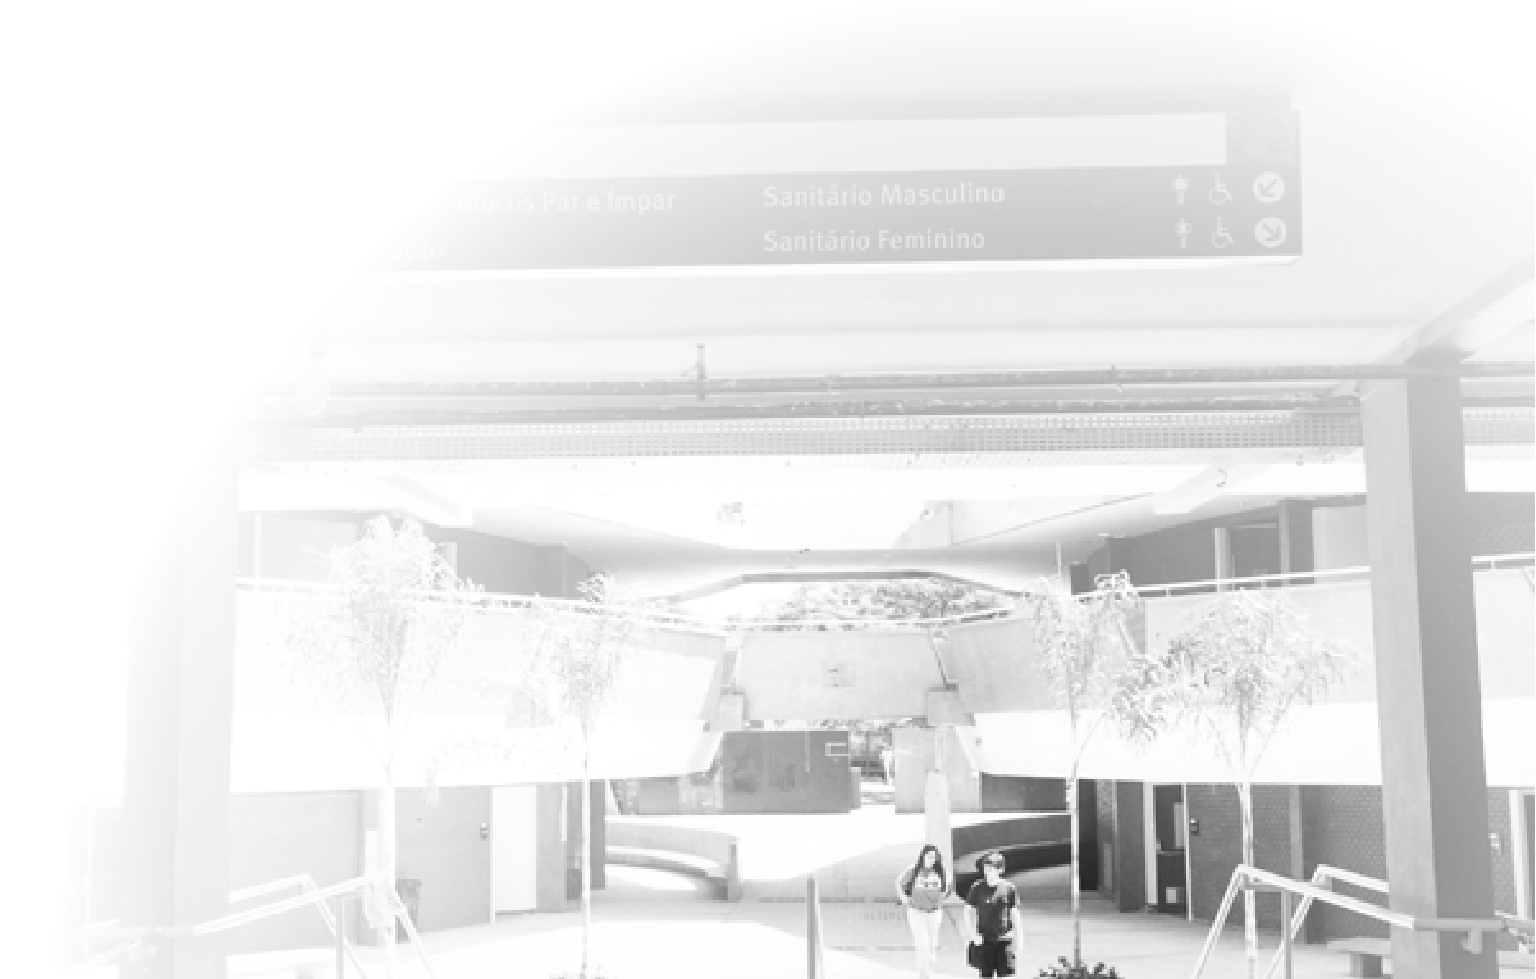
\includegraphics[width=.5\textwidth]{img/ola_mundo/cb.jpg}
\end{wrapfigure}

Olá, bixo! Seja bem-vindo! Agora que você está na faculdade, pode ser que
aprenda que aquele estereótipo de nerd da escola não lhe garante boas notas, e
que o lugar onde você mais vai aprender não necessariamente é a sala de aula. É
verdade, calouro, a faculdade é diferente, e quase tudo dependerá de você, desde
quais matérias quer cursar até quando vai estudar para as provas. Portanto, leia
isto com atenção.

Os professores, salvo raras exceções, dificilmente saberão seu nome ou quem é
você; provavelmente, eles só verão no final do semestre se o RA 137654  passou
ou não passou. Mas não se sinta desamparado, afinal, você também vai logo
esquecer a matéria deles! O quanto você estuda não é diretamente proporcional à
sua nota, portanto aprenda a estudar melhor. Atividades em grupo, resolução de
exercícios e monitorias são boas pedidas.

Mas a Universidade não se resume a estudo. Você vai conhecer muita gente nova e
descobrir que a vida acadêmica vai muito além.  Cada graduando tem uma cultura
própria, e tem gente do Brasil inteiro na Unicamp, então não se surpreenda se te
chamarem de pessoa, piá, meu, mano, jovem, moleque, guri, moço, rapaz, brou.
Essa diversidade é muito legal quando você se acostuma.

O campus é essa doideira toda mesmo. Você pode estar andando e cruzar com alguém
tocando gaita de fole, alguém parecendo uma estátua em plena praça, ou então um
grupo na grama lendo a Bíblia, treinando Wushu ou Taijiquan. Não se sinta
sozinho, afinal todos seus colegas estão assim também e depois de um mês você
estará adorando isso e perceberá porque todos dizem que a época de faculdade é a
melhor da vida.

Este manual foi organizado pelo CACo (Centro Acadêmico da Computação -- o seu
CA), para ajudá-lo nesse começo de vida universitária! Onde comer? Onde estudar?
Onde morar? Tudo isso são dúvidas comuns, que aqui tentamos ajudar a resolver.
Não há respostas prontas, cada um tem suas preferências, mas a gente dá uma mão.

O que é CA? E Atlética? E DCE? E Bandejão? E Moradia? E essas siglas e códigos
malucos? Como eu faço para pegar uma bolsa? A gente também tenta responder a todas
essas perguntas. E também damos algumas dicas de onde comprar coisas, onde se
divertir e alguns telefones úteis!

Parabéns pela aprovação! Seja bem-vindo e aproveite a vida acadêmica!

\clearpage

%%%%% Mensagem do diretor da FEEC
% Este arquivo .tex será incluído no arquivo .tex principal. Não é preciso
% declarar nenhum cabeçalho
\section{Mensagem da FEEC}  
 alunos, prezadas alunas, ingressantes no curso de Engenharia de Computação,

 Parabéns pela sua conquista, é com muita alegria que lhes acolhemos na UNICAMP
 e, em especial, na Faculdade de Engenharia Elétrica e de Computação (FEEC). A
 vida universitária é uma fase muito especial de nossas vidas: alguns poucos
 anos, tão intensos quanto breves, mas que costumam ser determinantes para
 nossas escolhas, para que forjemos nosso modo de agir, pensar e ver o mundo. É
 um percurso no qual cabe a vocês mesmos descobrir as nuances, as alternativas,
 procurando traçar, à medida em que caminham, as próprias metas pessoais.

 Numa carta de boas-vindas como esta, não conseguiria antecipar realidades para
 as quais cada um, cada uma, terá sua própria percepção. Também não gostaria de
 me deter em muitos conselhos, pois, tendo superado a dificílima etapa do
 vestibular, vocês já demostraram maturidade suficiente. Mas penso que não custa
 lhes falar sobre três aspectos que julgo importantes: dar-lhes a conhecer um
 pouco da FEEC e de sua história – história muito rica e da qual a partir de
 agora vocês fazem parte; apresentar o excelente curso que vocês agora começam;
 e, ao menos como sugestão para reflexão, tecer alguns comentários sobre a
 expectativa que a sociedade coloca nas pessoas que, como nós, temos ou tivemos
 o privilégio de fazer um curso de excelência numa universidade pública da
 qualidade da UNICAMP.

 Pode-se dizer que a FEEC começou oficialmente suas atividades acadêmicas no
 início de 1967, quando ingressou a primeira turma de Engenharia Elétrica da
 UNICAMP. Desde então, nossa Escola cresceu em pessoas, recursos e prestígio,
 consolidando-se como referência e liderança, tanto no ensino de graduação como
 de pós-graduação, ambos fortemente alicerçados na excelência de nossa atividade
 em pesquisa. Temos a felicidade de poder contar com um corpo docente de
 primeira linha, no qual convivem, em sinergia, a experiência de vários
 professores que praticamente começaram a FEEC com o dinamismo de jovens
 brilhantes que foram recentemente contratados. Temos também uma infraestrutura
 que, embora constantemente necessitada de melhorias, lhes dará as condições
 adequadas de estudo, tanto teórico como em laboratório. Mas sabemos que o
 melhor curso não se faz apenas com docentes e estrutura; temos consciência de
 que contamos, sobretudo, com os melhores estudantes. A partir de agora, vocês
 também fazem parte deste corpo discente que é o nosso principal diferencial. 

 O curso de Engenharia de Computação teve início em 1990, época em que nossa
 Escola já contava com grande prestígio, surgindo como uma consequência natural
 do bom nível da pesquisa que já realizávamos, à época, nesta área, e das
 necessidades de mercado de uma sociedade que começava a orientar-se
 intensamente para as tecnologias digitais, que hoje permeiam nossa vida. É um
 curso que já nasceu com o selo da excelência e da exigência. Compartilhamos
 este curso com os colegas do Instituto de Computação da UNICAMP, unidade de
 ensino e pesquisa do mais alto prestígio, na qual vocês também encontrarão um
 corpo docente extremamente qualificado. Como as demais engenharias, é um curso
 que requer uma base forte, de matemática e física. É importante aproveitar ao
 máximo esses primeiros semestres de curso básico, sem se deixar abater por
 dificuldades que são naturais, sem perder o “brilho nos olhos” desses primeiros
 dias de UNICAMP, tendo confiança de que, a despeito de limitações que sempre
 existem, o currículo de vocês é harmônico, está bem estruturado e lhes
 preparará de forma extremamente adequada para o futuro profissional.

 E, juntamente com os estudos, vocês descobrirão a partir de agora a vida
 universitária. A Universidade é também um lócus de cultura, debates e,
 sobretudo, momento único para se fazer amizades para a vida. Desejo que
 aproveitem muito bem cada instante de convivência, que participem com empenho e
 alegria das atividades e das entidades estudantis, nas quais vocês descobrirão
 um imenso leque de opções para contribuir com a universidade e, a partir dela,
 com o país. Mas desejo igualmente que não percam o foco no essencial que é a
 própria formação, de modo a não deixar arrefecer seus ideais, nem frustrar as
 expectativas que agora não são só de seus familiares, mas de toda a sociedade.
 A universidade, pública, gratuita e de excelência, passa por momentos difíceis.
 Nossas atividades se sustentam graças ao trabalho de milhões de cidadãos
 brasileiros, particularmente do Estado de São Paulo. Esta sociedade tem direito
 a nos cobrar eficiência, dedicação e qualidade, a nós, gestores e professores,
 mas também aos estudantes, cujo comprometimento ético deve se pautar pela
 dedicação ao aprendizado, vencendo a tentação do desânimo, por fomentar o
 desejo de saber sempre mais, qualificando-se assim para, no futuro, por meio de
 seu trabalho profissional, dar o justo retorno a quem nos financia.

 Eu termino com uma citação que gosto muito, é de um autor clássico da
 antiguidade grega, Píndaro, que num de seus versos dizia: “torna-te aquilo que
 tu és”. É um chamado do poeta para que o leitor tome consciência de quem é, de
 aonde está, e saia assim de um possível momento de alienação ou prostração.
 Vocês são hoje estudantes ingressantes do curso de Engenharia de Computação da
 UNICAMP. Não é pouca coisa! São certamente orgulho para seus familiares e agora
 também patrimônio de nossa Escola. Desejo sinceramente que tenham esta
 realidade sempre presente ao longo dos anos em que estiverem aqui. Desde já
 coloco a diretoria da FEEC e as coordenações de curso para lhes apoiar neste
 sentido, em toda e qualquer dificuldade que possam ter. Sejam bem-vindos, sejam
 bem-vindas à FEEC e, sobretudo, sejam muito felizes aqui conosco.

 João Marcos Travassos Romano
 Diretor da FEEC

\clearpage

%%%%% Mensagem do diretor do IC
% Este arquivo .tex será incluído no arquivo .tex principal. Não é preciso
% declarar nenhum cabeçalho

\section{Mensagem do IC}

Caros Alunos,

Sejam bem-vindos à Unicamp e ao Instituto de Computação (IC). 

Parabenizo a todos vocês pela conquista em estarem nesta instituição. No ano de
2014, o IC celebrou os 45 anos da Computação na Unicamp, um dos cursos mais
antigos do Brasil. Vale destacar que, desde sempre em sua trajetória, os nossos
cursos são reconhecidos dentre os melhores.  Trata-se de cursos de excelência
que reúnem com muita frequência os melhores alunos de várias escolas do Brasil e
que contam com professores com significativa atuação acadêmica e científica.

Neste momento se inicia uma nova etapa na vida de cada um: novo ambiente, novos
amigos, novos desafios, novas possibilidades; tudo isso acompanhado de mais
liberdade, independência e responsabilidade.  O ambiente universitário, vocês
verão, é extremamente fértil; oferece não apenas oportunidades acadêmicas de
qualidade (como aulas, palestras, mini-cursos, visitas técnicas e científicas,
estágios e atividades de iniciação científica), como também um universo de
experiências extracurriculares (Atlética, Centro Acadêmico, Bateria Valorosa,
Empresa Júnior, feiras de recrutamento, olimpíadas e maratonas de programação,
etc.) que possibilitam momentos inspiradores para aquisição de conhecimento,
maturidade e aperfeiçoamentos pessoal e profissional. Muitas destas atividades
extracurriculares são oferecidas ao mesmo tempo e não são raras as situações em
que conflitam com as atividades acadêmicas regulares. O principal desafio é
aprender a escolher e planejar, a gerenciar o tempo e os interesses, a cuidar
das relações pessoais, a considerar os prós e contras. Estejam atentos...

O que tenho para dizer a vocês, de ainda maior relevância, é algo que
erroneamente deixamos para o final da trajetória acadêmica quando, na verdade,
deveria ser a motivação de todas as nossas ações e que deveria permear todas as
nossas escolhas:

\begin{enumerate}
\item Sejam autores de suas próprias histórias;

\item Deixem vir à superfície a melhor versão de vocês mesmos;

\item Guiem-se pelos preceitos do Bem e do Belo e os defendam com a convicção de
  estarem colaborando pela alegria de se viver;

\item Não se acostumem nunca com aquilo que gostariam de mudar, com o que
  gostariam de romper, com o que lhes conduz para fora de seus caminhos no
  encontro consigo mesmos.
\end{enumerate}

Isso é o que devemos dizer para vocês, caros alunos, a todo instante durante
seus percursos nesses anos de universidade; é isso o que devemos dizer sempre a
nós mesmos enquanto docentes, orientadores, pesquisadores, cidadãos, enfim, como
pessoas. Proponho um desafio: que todos nós nos engajemos em perseguir e
converter em atos essas palavras; proponho que cada um de nós nos compromissamos
a transpor a preguiça, a desesperança, o medo, a incompreensão, a rivalidade sem
sentido, etc..., e busquemos realizar com responsabilidade o que nos faz
felizes, simplesmente. E que esse estado de contentamento irradie.

Parabéns a todos pela trajetória que se segue a partir daqui.

Ricardo da Silva Torres

Diretor,

Instituto de Computação,

Unicamp
\clearpage

\twocolumn
%%%%% Para pensar
% Este arquivo .tex será incluído no arquivo .tex principal. Não é preciso
% declarar nenhum cabeçalho

\section{Para pensar}

O objetivo desse tópico não é responder grandes questões, nem doutrinar ninguém,
apenas expor alguns assuntos que achamos importante que você, bix*, analise
neste momento em que você está iniciando sua vida na universidade.

\subsection*{Unicamp, uma Universidade Pública?}

À primeira vista, um título como esse pode parecer estranho. ''Mas como? Acabei
de entrar na Unicamp, uma universidade estadual e não vou pagar mensalidades
para estudar nela. É óbvio que ela é uma Universidade Pública.'' Será?

Público, no sentido do dicionário, refere-se a ''tod*s'', ao ''povo'', mas
também no sentido popular quando nos referimos a algo público, logo lembramos de
acesso irrestrito e gratuito, sem distinção alguma a tod*s *s cidadãos e
cidadãs, um lugar que tod*s tem direitos de usufruir. Mais ainda, público
significa que tod*s pagam, que é gerido e que foi construído com o dinheiro de
todas as pessoas através dos impostos arrecadados pelos mecanismos do Estado. É
isso que acontece por exemplo com os hospitais, creches e escolas públicas que,
embora possuam atendimento muitas vezes precário, atendem a tod*s.

Mas e uma universidade, de que forma ela se encaixa dentro do ''público''?

\begin{figure}[h!]
    \centering
    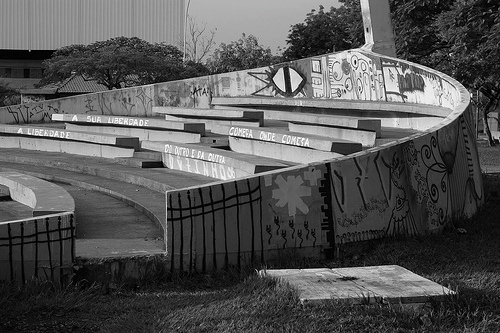
\includegraphics[width=.45\textwidth]{img/ola_mundo/teatro_de_arena.jpg}
\end{figure}

Para responder melhor essa questão, devemos analisar a universidade com base em
seu tripé essencial: ensino, pesquisa e extensão. Comecemos por analisar o
acesso ao ensino. Por um lado, o processo seletivo da universidades públicas
paulistas, o vestibular, é uma forma virtualmente imparcial de seleção, que deve
analisar apenas o nível de conhecimento d* candidat* (que muitas vezes está
ligado ao valor de sua renda), sem levar em conta a religião, o sexo ou a classe
social d* vestibuland*. Logo, exceto por pontos extras (para negr*s, índi*s e
estudantes de escola pública), para ingressar pelo vestibular em uma
universidade como a Unicamp não há nenhuma distinção entre *s cidadãos e
cidadãs. Por outro lado, só no Estado de São Paulo há cerca de 2 milhões de
jovens com idade para estar na universidade, enquanto isso as três universidades
estaduais paulistas (USP, UNESP e Unicamp) não chegam a oferecer 100 mil vagas
de graduação e pós. Portanto, nem 5\% d*s jovens paulistas tem acesso ao ensino
público superior, sendo que a grande maioria d*s ingressantes na universidade
pública pertence às classes média ou alta.

Agora, tendo em mente a pesquisa, podemos dizer que a Unicamp se destaca nesse
ponto: Ela é responsável por 15\% de toda a pesquisa brasileira, desenvolve
vários estudos sobre a sociedade brasileira (tendo publicado recentemente um
atlas social), projetou equipamentos de segurança para carros, está trabalhando
em sistemas computacionais para saúde, entre tantas outras pesquisas voltadas
para o progresso da ciência e tecnologia nacional. Isso, sem contar que a
Unicamp é a universidade que mais registra patentes no Brasil. Mas grande parte
dessas patentes são vendidas a grandes empresas, muitas vezes multinacionais.
Outro ponto crítico existente são as pesquisas particulares desenvolvidas na
Unicamp (no IC, por exemplo, há projetos de pesquisa com empresas como Samsung,
Microsoft e IBM onde as patentes são divididas entre universidade,
pesquisador(a) e empresa).

Finalmente, falaremos sobre a extensão. Na nossa universidade o principal
projeto de extensão é a administração de hospitais da região como o HC, que é o
maior hospital público do interior paulista e atende pessoas de toda a região e
até de fora do Estado. Fora ele, a universidade não desenvolve nenhum projeto de
extensão gratuito que tenha grande destaque. No Instituto de Computação, por
exemplo, os cursos de extensão custam mais de R\$ 5000,00 por alun*, o que não
pode realmente ser chamado de extensão universitária, uma vez que não está
distribuindo à comunidade o conhecimento produzido aqui dentro.  Além disso a
Unicamp também restringe o acesso a diversos espaços da universidade, como por
exemplo o controle do acesso noturno ao campus, a coibição de festas e a
dificuldade de acesso aos espaços da Faculdade de Educação Física. Outras
universidades como a UNESP e a USP Leste tem uma política bem melhor de
extensão.

Resgatar o sentido do público tanto conceitual quanto materialmente se faz
sempre necessário. Assim, desde já, participe das discussões do Centro Acadêmico
e de outras organizações estudantis que achar conveniente para questionar as
deficiências e produzir novos caminhos para formarmos com a colaboração de tod*s
uma universidade cada vez mais pública.

\subsection*{Eu, um(a) estudante da rede pública?}

Você já parou para pensar o que está começando a ocorrer em sua vida? A partir
de agora você estuda em uma universidade pública, ou, como já foi dito, a partir
de agora o povo está pagando para você estudar. E o que você fará com esse
privilégio?

\begin{figure}[h!]
    \centering
    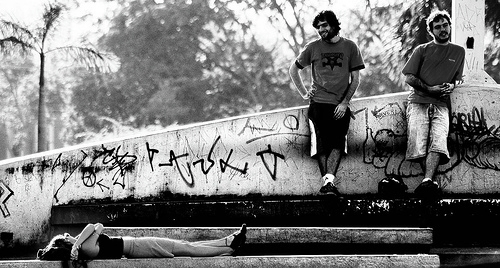
\includegraphics[width=.45\textwidth]{img/ola_mundo/teatro_de_arena1.jpg}
\end{figure}

Se você for perguntar, encontrará milhares de maneiras de encarar o fato de ser
um(a) estudante da rede pública, e provavelmente algumas das respostas
provavelmente incluiriam um pouco das visões a seguir:

Algumas pessoas veem a aprovação como o último passo do desafio de entrar na
universidade, uma conquista pessoal, e, desta maneira, a única pessoa a quem
est*s tem de prestar contas sobre o que fizeram de seus estudos na Unicamp
seriam el*s mesm*s. Outr*s acreditam que estudar em uma universidade pública
traz uma responsabilidade direta: estudar corretamente. Um(a) alun* da Unicamp
teria de aproveitar a universidade ao máximo, buscando sempre aprender, para que
saia daqui como um(a) profissional competente para auxiliar o progresso
tecnológico da nossa sociedade, de modo a cumprir com o papel que lhe foi
atribuído. Também existem algumas pessoas que acreditam que assim que entramos
na universidade nos tornamos agentes públicos. Sendo assim, além de estudar
também seria papel d* alun* interagir constantemente com a comunidade passando a
ela os conhecimentos que a universidade lhe proporcionou, buscando criar um elo
universidade-comunidade.

Afinal, qual dessas visões seria a mais correta sobre o que é um(a) estudante da
rede pública? Essa é uma resposta que não daremos aqui (até porque, como foi
dito no início, respostas não fazem parte do objetivo deste tópico), ela é algo
individual. Mas seria bom que você pensasse qual a razão pela qual você está na
Unicamp e qual o objetivo da sociedade quando ela paga para que você tenha essa
oportunidade.

E, bix*, nunca é demais desejar: Que você faça o melhor proveito do seu tempo
aqui na Unicamp!


\chapter{Sobrevivendo em Barão}
%%%%% Lugares para morar
% Este arquivo .tex será incluído no arquivo .tex principal. Não é preciso
% declarar nenhum cabeçalho

\section{Lugares para morar}

O custo de moradia em Barão Geraldo depende principalmente de três fatores:
proximidade da Unicamp, tamanho do imóvel e qualidade da casa (acabamento,
número de banheiros, presença de piscina etc.) Quanto à distância, os entornos
da \textbf{Avenida 1} (Avenida Doutor Romeu Tortima) e da \textbf{Avenida 2}
(Avenida Professor Atílio Martini) costumam ser mais caros de se morar, por
serem próximos da Unicamp. A região que vai do centro de Barão Geraldo até a
Moradia Estudantil, um pouco mais distante da universidade (cerca de 10 minutos
de bicicleta), é em geral mais barata e concentra muito mais serviços, como
supermercados, restaurantes e bancos.

Uma boa dica para se informar a respeito de lugares para morar (repúblicas,
quitinetes, pensionatos) é o site \textbf{Morar Unicamp}
(\url{morarunicamp.com.br}), criado por alunos. Lá você encontra informações
como endereço, preço, contato e detalhamento do lugar.

\subsection{Moradia Estudantil}

A \textbf{Moradia} é um exemplo de conquista de todos os estudantes. O processo
de reivindicação de uma moradia estudantil para a Unicamp começou com o
movimento Taba. Durante dois anos, alunos ficaram acampados no CB (Ciclo Básico)
até que as obras começassem. Hoje em dia, graças à Moradia, várias pessoas que
não teriam condições de se manter em Campinas pagando aluguel podem estudar na
Unicamp.

\begin{figure}[h!]
    \centering
    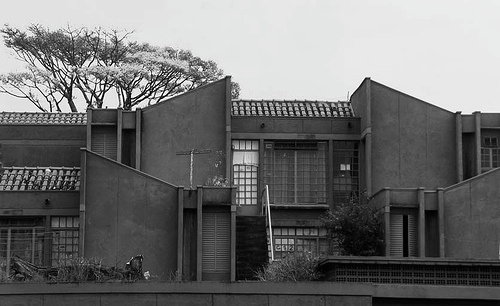
\includegraphics[scale=0.55,keepaspectratio=true]{img/imgs/5-moradia/-029.jpg}
\end{figure}

A Moradia existe desde 1989. De lá para cá, o número de vagas em cursos da
Unicamp aumentou muito e as vagas da Moradia tornaram-se insuficientes para
acomodar todos que precisam. A reivindicação de mais vagas para a Moradia é uma
das principais bandeiras do DCE e um desejo de muitos estudantes.

Cada casa da Moradia, normalmente dividida por quatro pessoas, constitui-se de
um quarto, uma cozinha, um banheiro e uma sala. Há ainda o Ônibus da Moradia, um
circular da Unicamp que transporta pessoas durante o dia todo da Moradia até a
Unicamp e vice-versa.

A Moradia está localizada na Avenida Santa Isabel, 1125, a cerca de 3 km do
campus.

Para saber mais sobre a Moradia e o processo seletivo, entre no site
\url{www.pme.unicamp.br}.

\subsection{Repúblicas}

A melhor escolha, se você tiver condições de pagar por uma moradia.

\begin{figure}[h!]
    \vspace{-10pt}
    \centering
    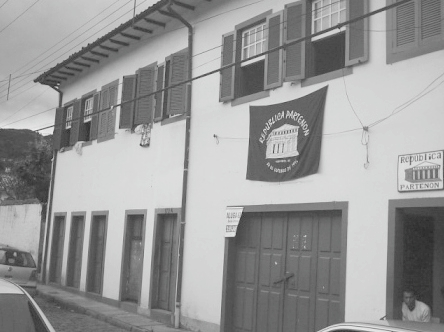
\includegraphics[scale=0.58,keepaspectratio=true]{img/imgs/5-moradia/-034.jpg}
    \vspace{-10pt}
\end{figure}

Você pode levar quem quiser para sua casa, chegar no horário que bem entender,
além do que você conhecerá muita gente nova. Se possível, more em uma república
de cursos mistos, pois assim você terá contatos diversos.

O custo de uma vaga em república é muito variável, a depender do conforto que
você espera e da localização. Gira em torno de R\$ 475 para dividir quarto com
outras pessoas e R\$ 650 para um quarto individual. Esses valores já são a soma
do aluguel com despesas adicionais (água, luz, limpeza etc.)

Escolha bem as pessoas com quem você vai morar para não ter problemas com
diferentes estilos de vida. Tem gente que gosta de lavar louça a cada 5 minutos
e tem gente que usa o chão como lata de lixo tranquilamente. Veja com quem você
se dá melhor.

\subsection{Quitinetes}

Cuidado! A especulação imobiliária em Barão Geraldo chega a ser imbecil. As
quitinetes mobiliadas são normalmente compostas de um banheiro e um cômodo que é
quarto, sala, cozinha e área de serviço. Os valores de aluguel são da ordem de
R\$ 1000 ou mais. Sim, mil reais por um microespaço. Só porque é perto da
Unicamp. Fique de olho e tome cuidado com os contratos.

\begin{figure}[h!]
    \centering
    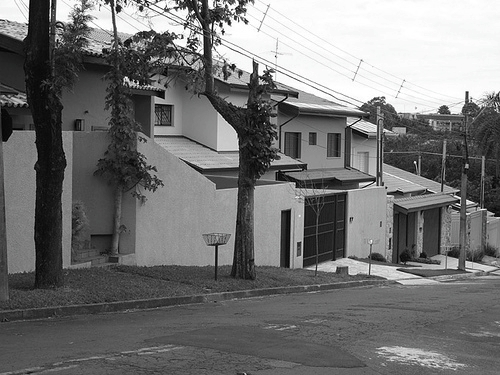
\includegraphics[scale=0.55,keepaspectratio=true]{img/imgs/5-moradia/-033.jpg}
\end{figure}

As melhores relações custo-benefício de quitinetes são as daquelas próximas ao
centro de Barão Geraldo ou no espaço entre as avenidas. E lembre-se de que não é
só de Unicamp que se vive. Não adianta pagar mais caro para estar do lado da
universidade, se você fica muito longe dos supermercados, farmácias etc.

\subsection{Pensionatos}

Pensionatos são como repúblicas, só que com regras. Muitas regras. Dependendo do
pensionato que você conseguir, pode tornar-se uma grande roubada. Alguns não
deixam você levar pessoas para casa, reclamam se você chegar tarde e não liberam
festas; outras, não, então procure bem.

O preço fica por volta de R\$ 625 para dividir quarto e R\$ 850 para quarto
individual. Pode ser uma opção muito cômoda se você procura um conjunto de casa,
comida e roupa lavada.

É muito importante que você saiba que contratos de um ano (ou qualquer período)
em pensionatos são ilegais e você não precisa cumpri-los.

\subsection{Segurança}

Por ter muitas casas de famílias abastadas e de estudantes (em geral
desatentos), Barão Geraldo é grande alvo de assaltos a residências e, além
disso, o distrito peca pela falta de segurança.

Não é raro ouvir que alguém foi assaltado enquanto voltava para casa à noite
sozinho ou que teve a casa saqueada durante um feriado prolongado. Mais
chocantes ainda são os casos de estupro de moças que ocasionalmente são
divulgados em grupos de e-mail e redes sociais. Cuidado! É importante zelar pela
sua integridade e pela de seus pertences -- assim como seus pais fazem em sua
casa, não importa onde eles morem.

\begin{figure}[h!]
    \centering
    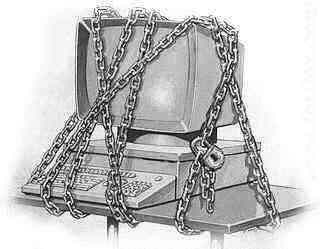
\includegraphics[scale=0.55,keepaspectratio=true]{img/imgs/5-moradia/seguranca.jpg}
\end{figure}

Evite andar sozinho à noite, especialmente nos fins de semana. Se o seu
pensionato ou a sua república paga o segurança da rua, o que é altamente
recomendável, use \emph{sempre} de seus serviços, seja ligando para pedir
escolta ao chegar em casa ou para avisar caso ouça algum barulho suspeito.

Ao voltar para sua cidade em feriados prolongados, deixando a casa vazia, não se
esqueça de trancar todas as portas e janelas de casa, verificar se não há nada
no quintal que possa ser levado facilmente (colocar as bicicletas e aparelhos de
som na sala é uma boa ideia) e trancar os objetos de valor (computadores,
televisões) dentro dos quartos.

\subsection{Imobiliárias}

\begin{itemize}
    \item   \textbf{Imobiliária Barão Housing}
        \\Telefone: (19) 3289-4113
        \\Endereço: Rua Tranquilo Prosperi, 383
        \\E-mail: \email{atendimento@baraohousing.com.br}
        \\Site: \url{baraohousing.com.br}

    \item   \textbf{Imobiliária Lanza}
        \\Endereço: Rua Benedito Alves Aranha, 104
        \\Telefone: (19) 3289-1717 / (19) 3307-7155
        \\E-mail: \email{lanza@lanzaimoveis.com.br}
        \\Site: \url{lanzaimoveis.com.br}

    \item   \textbf{Imobiliária Professor Sebastião}
        \\Endereço: Av. Dr. Romeu Tortima, 344
        \\Telefone: (19) 3289-2317
        \\E-mail: \email{ipsimoveis@ipsimoveis.com.br}
        \\Site: \url{ipsimoveis.com.br}

    \item   \textbf{Amaral Imóveis}
        \\Endereço: Av. Dr. Luiz de Tella, 864
        \\Telefone: (19) 3287-0655 / (19) 4141-1010
        \\E-mail: \email{amaral@amaralimoveis.net}
        \\Site: \url{amaralimoveis.net}

    \item   \textbf{Zaine Conquista Imóveis}
        \\Endereço: Av. Santa Isabel, 84
        \\Telefone: (19) 3289-4050 / (19) 3289-2761
        \\E-mail: \email{zaine@correionet.com.br}
        \\Site: \url{zaineconquista.com.br}

    \item   \textbf{Ismê Assessoria Imobiliária}
        \\Endereço: Rua Christina G. Miguel, 250
        \\Telefone: (19) 3289-4325
        \\E-mail: \email{isme@isme.com.br}
        \\Site: \url{isme.com.br}

    \item   \textbf{Rute Svartman Imóveis}
        \\Endereço: Rua Engenheiro Edward de Vita Godoy, 850
        \\Telefone: (19) 3368-0881
        \\E-mail: \email{imoveis@rutesvartman.com.br}
        \\Site: \url{rutesvartman.com.br}

    \item   \textbf{Imobiliária Ávila \& Ferraris}
        \\Endereço: Av. Dr. Romeu Tortima, 714
        \\Telefone: (19) 3289-3522
        \\E-mail: \email{dcaavila@terra.com.br}
        \\Site: \url{avilaeferrarisimoveis.com.br}

    \item   \textbf{Imobiliária Cidade Universitária}
        \\Endereço: Av. Dr. Romeu Tortima, 624
        \\Telefone: (19) 3289-3322
        \\E-mail: \email{contato@cidadeuniversitariaimoveis.com.br}
        \\Site: \url{cidadeuniversitariaimoveis.com.br}

    \item   \textbf{Denilson Imóveis}
        \\Endereço: Av. Dr. Luís de Tella, 55
        \\Telefone: (19) 3289-1444
        \\E-mail: \email{contato@denilsonimoveis.com.br}
        \\Site: \url{denilsonimoveis.com.br}

    \item   \textbf{Mega Barão Imóveis}
        \\Endereço: Rua Francisca Resende Merciai, 103 B
        \\Telefone: (19) 3289-7101 / (19) 3386-4141
        \\E-mail: \email{megabarao@megabaraoimoveis.com.br}
        \\Site: \url{megabaraoimoveis.com.br}

    \item   \textbf{Libano Imóveis}
        \\Endereço: Rua Francisca Resende Merciai, 90
        \\Telefone: (19) 3789-9999
        \\E-mail: \email{contato@libanoimoveis.com.br}
        \\Site: \url{libanoimoveis.com.br}

    \item   \textbf{Marco Imóveis}
        \\Endereço: Rua José Pugliesi Filho, 420
        \\Telefone: (19) 3287-8083
        \\Site: \url{marcoimovel.com.br}

    \item   \textbf{Lokal Imóveis}
        \\Endereço: Rua José Próspero Jacobucci, 290
        \\Telefone: (19) 3256-4616

    \item   \textbf{Carpe Diem Imóveis}
        \\Endereço: Av. Dr. Romeu Tortima, 184
        \\Telefone: (19) 3579-5655 / (19) 3304-9323
        \\Site: \url{carpediemimoveis.com.br}

    \item   \textbf{Cássio Carvalho Imóveis}
        \\Endereço: Av. Santa Isabel, 750
        \\Telefone: (19) 3288-0143
        \\E-mail: \email{cassio@cassioimoveis.com.br}
        \\Site: \url{cassioimoveis.com.br}

    \item   \textbf{Delphos Empreendimentos Imobiliários}
        \\Endereço: Av. Albino J. B. de Oliveira, 830
        \\Telefone: (19) 3289-5353

    \item   \textbf{Roma Imóveis}
        \\Endereço: Rua Agostinho Pattaro, 222
        \\Telefone: (19) 3287-9118

    \item   \textbf{Valter Imóveis}
        \\Endereço: Rua Maria Ferreira Antunes, 22
        \\Telefone: (19) 3289-6088

    \item   \textbf{Imobiliária Marco Antônio}
        \\Endereço: Av. Dr. Romeu Tortima, 1522
        \\Telefone: (19) 3287-6663
\end{itemize}

E pela quantidade de imobiliárias vistas, dá para ter uma ideia de como a 
especulação imobiliária come solta em Barão.
\newpage
%%%%% Comida
% Este arquivo tex vai ser incluído no arquivo tex principal, não pe preciso
% declarar nenhum cabeçalho

\section{Comida}
\subsection{Bandejão}

Um dos momentos de glória do dia de um futuro engenheiro, cientista ou bacharel
é o Bandejão. É a hora de intensas e indiscutíveis emoções. Caso sua salada
corra sobre a mesa, mantenha-se calmo. Evite discussões, jamais tente descobrir
o sabor do suco pelo paladar (caju ou manga?). É mais cômodo ler no cardápio do
dia. Uma dica: para cortar o bife faça muita força e, quando começar a amolecer,
pare, você chegou na bandeja.

Falando sério agora: o Bandejão (Restaurante Universitário), ou Bandeco,
fica ao lado da Biblioteca Central, bem em frente ao PB (Prédio Básico, ou Ciclo
Básico II) e, a menos que você não queira economizar uma boa grana com comida,
vai ser o lugar onde você vai estar na maioria dos seus horários de almoço. Com
o tempo, você vai ver que o Bandeco é o ``coração da Unicamp''. É o local de
você se encontrar com os amigos (combinando ou não antes), contar os micos nas
aulas, jogar conversa fora e falar mal da comida, que nem é tão ruim assim como
muitos dizem. Sem dúvida, é o melhor custo-benefício da Unicamp. Por R\$2,00,
você tem direito a arroz, feijão, pão, salada, proteína de soja, suco, chá e café à
vontade. A carne e a sobremesa tem que dar uma choradinha para a tiazinha para
poder repetir, mas geralmente dá certo.

\begin{figure}[h!]
    \centering
    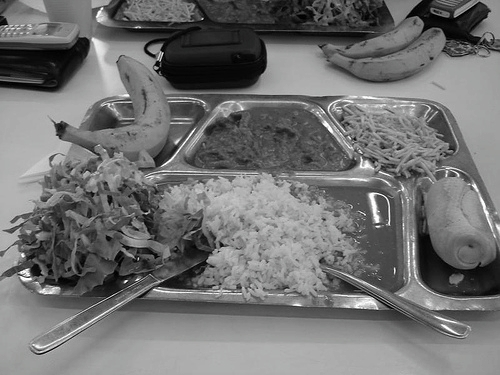
\includegraphics[width=.45\textwidth]{img/barao/bandeco.jpg}
\end{figure}

Existe também o RA (Restaurante Administrativo, não confundir com registro acadêmico), também conhecido como Prateco,
pelo fato de a comida ser servida em pratos e não em bandejas. Fica atrás da
Faculdade de Engenharia Elétrica e de Computação (FEEC), perto do prédio da
Engenharia Básica. Tem algumas diferenças em relação ao Bandeco: o espaço físico
é bem menor, por exemplo. No RA você mesmo se serve, apesar de a carne
ser servida pela tia que trabalha lá. Dependendo
de onde você vai ter aula antes ou depois do almoço, é mais negócio almoçar no
RA. Para poder usar o Bandeco e o RA, você deve estar com o seu Cartão
Universitário (também chamado de RA) carregado.

Além do RA, há o novo restaurante universitário, conhecido como RS (Restaurante
Universitário da Saturnino). Ele é localizado próximo ao IC-3 e ao prédio azul
da Civil. Semelhante ao RA, você come em pratos, as tias servem a carne e o
resto é self-service. As vantagens são que o ambiente é menos claustrofóbico, há
mais lugares e a localização o torna muito prático para os computeiros. Porém,
só está aberto no período do almoço. Desconsiderando a localização, o RS com
certeza é a melhor opção no almoço.

Um cardápio ovo-lacto-vegetariano está sendo oferecido desde o fim de 2013. Ele
está disponível no RS (ou seja, somente no almoço), numa fila separada. Agora, é
possível saborear pratos tais como abobrinha agridoce, hambúrguer de soja,
legumes com molho branco, torta de aveia, entre outros.

\subsubsection*{Como funciona o esquema de carregar o cartão?}

Simples. Você vai à uma das máquinas que existem na entrada dos restaurantes e
faz, por exemplo, um depósito de R\$20,00 para 10 créditos. As máquinas aceitam
apenas notas, e sem troco. Outra maneira de colocar créditos é fazer um depósito
na conta do Bandeco no Santander (Ag.: 207 / Conta: 43.010.009-2) ou no Banco do
Brasil (Ag.: 4203-X / Conta: 66.315-8) e depois carregar o seu cartão, na
Prefeitura do Campus (próximo à Reitoria), apresentando o comprovante de
depósito. Não são aceitos comprovantes de pagamento de entrega de envelope ou
via internet.

Os restaurantes funcionam de segunda a sexta, nos seguintes horários:

\begin{itemize}
    \item  RU, das 10h30 às 14h (almoço) e das 17h30 às 19h45 (jantar).
    \item  RA, das 11h30 às 14h (almoço) e das 17h30 às 19h (jantar).
    \item  RS, das 11h30 às 14h (almoço).
\end{itemize}

Em períodos especiais, como fim de ano, os restaurantes podem funcionar em
horários reduzidos, alguns não abrem, ou então fecham completamente, fique de
olho nos emails e informes que você recebe.

Para saber previamente o cardápio do Bandejão, acesse o site da Prefeitura do
Campus (\url{prefeitura.unicamp.br}) ou o GDE (\url{gde.ir}).

Para Android e iOS, está disponível o aplicativo Unicamp Serviços, do CCUEC, que
informa cardápio e saldo no seu cartão, entre outros.

\subsection{Outros lugares para as refeições}

Algumas opções dentro da Unicamp são:

\begin{itemize}
\item Cantina do DCE: tem self-service barato e com variedade no almoço.
\item Cantina da FEA/FEM: próxima a FEEC, também tem self-service no almoço. Pra
  quem não gosta de café, fica a dica da latinha de Red Bull a R\$ 5,99.
\item Gatti: Se você é vegetariano, é uma boa dica. Fica do lado do IC-2, na
  Cênicas/Dança.
\item Cantina da Biologia: Tem self-service e marmita.
\item Cantina da Química:  Tem prato-feito, abre também aos sábados.
\item Cantina da Educação: Tem self-service.
\end {itemize}

Fora da Unicamp:

\begin{itemize}
\item Terraço: próximo ao balão da Av. 1, vende marmitex e tem self-service a um
  preço bom, além de churrasco às terças, quintas e sábados.
\item Bardana: Um pouco mais acima na Av. 1, com a fachada toda verde. Está na
  mesma faixa de preço do Terraço, e costuma ser considerado bem melhor; tem
  churrasco de carne bovina meio que dia-sim-dia-não, e nos outros dias é de
  frango. No jantar, há pratos à la carte, e pizza.
\item Pepe Loco: serve comida mexicana no estilo fast-food. Porém costuma ser
  bem caro pela qualidade e quantidade que oferece.
\item Aulus: na Av. 2, próximo ao balão, que é o mais caro dos citados aqui, mas
  é muito bom (e bonito). O cardápio geralmente inclui peixes e frutos do mar, e
  tem churrasco todo dia.
\item Campus Grill: em frente à guarita do HC, comida boa a um preço um tanto
  alto.
\item Outros: Na frente da reitoria há o Del Sol, o Ginza e o Moriá.  O Del Sol
  serve comida por quilo, sendo parecido (em preço e pratos) com o Bardana,
  enquanto que o Ginza serve a la carte com preços bons e o Moriá serve pratos
  feitos a preços mais baratos. 
\end{itemize}

\subsection{Lanches e sucos}

Tá de tarde, bateu fome, quer comer um lanche (hamburger, pão-na-chapa, queijo
quente, x-salada, croissant, qualquer coisa do gênero)? Quase todas as cantinas
da Unicamp servem lanches. Algumas muito boas são a cantina da Mecânica e a
lanchonete da Economia.

Se você estiver no IC quando bater a fome, as opções mais próximas são a cantina
da Economia e a do Gatti. Perto da FEEC existem a Padaria da FEA e a Cantina da
Mecânica. Já nas redondezas do CB existe a cantina do DCE.

Quase todas as cantinas servem salgados prontos, lanches naturais, doces e
demais coisas do gênero.

Para sucos, tem um lugar muito bom: a famosíssima banca de sucos do CB, que tem
milhões de sucos, vende frutas e também salgados.  Se você precisa almoçar
rápido, provavelmente sua escolha será salgado + vitamina na banca de sucos do
CB. Todo dia a banca de sucos do CB tem um sabor na oferta, que é ótimo pra sair
do tradicional suco de laranja.

Nas quartas e quintas há uma feira no centro da praça do CB, na qual há opções bem
variadas, desde pastéis a comida japonesa, embora geralmente mais caras que as
cantinas. Uma opção interessante é o Porqueta, que serve costelinhas de porco
assadas e sanduiches muito bem feitos, mas é um pouco caro.

Açaí: a cantina da física tem um açaí na tigela, caro, mas bom. Se por algum
motivo você tiver de andar até o quarteirão de salas de aula da medicina,
estiver cansado, e quiser um açaí, o da cantina de lá é caro e
inacreditavelmente zoado. O açaí com melhor custo-benefício da Unicamp é o da 
feirinha, mas só existe as quartas e quintas, então aproveite nesses dias para
matar sua vontade.


\subsection{Padarias e café da manhã}

Duas cantinas da Unicamp abrem bem cedo e servem o bom pingado + pão na chapa
matinal. São elas a Mecânica e a cantina do DCE.

\subsubsection{Padaria Alemã}

A Padaria Alemã, na Av. 1, próxima ao Dalben, serve uma bandeja de café da manhã
com suco, café-com-leite/chocolate, croissant, mamão, bolo, pão francês,
torradas, manteiga e geleia. Ainda há a possibilidade de fazer trocas como: suco
por chocolate, croissant por dois pães-na-chapa, mamão por banana, coisas do
gênero.
\begin{figure}[h!]
    \centering
    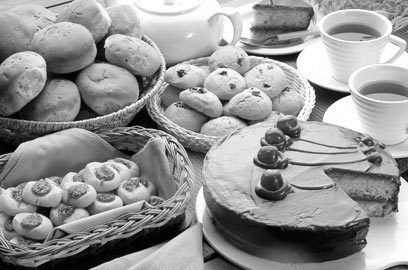
\includegraphics[width=.45\textwidth]{img/barao/padaria.jpg}
\end{figure}

Também são servidos lanches gigantescos, com muitas opções de recheio, por um
preço relativamente barato, então tenha alguém para dividir se sua fome não for
muita (acredite, meio lanche já serve como um almoço completo). Dependendo do
recheio, a pizza é muito barata, também, embora eles não façam entrega. É bom
lembrar que eles servem café da manhã das 7h até às 13h (mas a padaria só fecha
às 22h), então é uma boa pedida para se você não quiser almoçar ou para sábado e
domingo, acordar tarde e tomar um café da manhã para valer pelo almoço.

\subsubsection{Paneteria Di Capri}

Na Estrada da Rhodia, próximo à entrada da Cidade Universitária II, há a
Paneteria Di Capri, que tem um pão francês muito bom (a um preço legal) e também
muita variedade (incluindo tortas e lanches).

Além disso você também pode tomar seu café da manhã lá, pois como quase toda
padaria eles também oferecem um cardápio bom para logo cedo. Se você estiver com
bastante apetite, de sexta a domingo eles servem um buffet de café da manhã com
muitas opções e a um preço fixo (em torno de R\$12).

Na hora do almoço também são preparados alguns pratos (para comer no local e
para levar) e também há um esquema onde você pede um grelhado e tem acesso livre
a um balcão com saladas e outras coisas, como petiscos. À noite eles servem
pizzas e também há o esquema do grelhado, exceto no inverno, quando eles servem
um buffet de sopas.

\subsubsection{Padaria da FEA}

Já se você está na Unicamp e quer uma padaria, a dica é a Padaria da FEA (fica
próxima à Cantina da Mecânica). Lá eles têm pães, doces e bolos. Com uma
diferença: há produtos especiais, como pão de queijo com linhaça ou alho e pão
francês com soja. Mas não se assuste: por mais estranho que pareçam, os produtos
de lá são muito bons! E não deixe para ir lá depois das aulas, pois a Padaria da
FEA fecha às 17h.

\subsection{E no fim de semana?}

Nos fins de semana, nem o Bandex nem quase nenhuma cantina da Unicamp abrem (e
só no sábado, se abrirem). Você vai ter que se virar fora da Unicamp.

Na Av. 1 e proximidades tem o Terraço, o Bardana e a Padaria Alemã já citados,
além de vários restaurantes próximos à Alemã.

Na Av. 2 tem o Aulus, mais caro no sábado que durante a semana; domingo, então,
mais ainda, mas costuma ter camarão à milanesa; porém a marmita tem opções de
carne e acompanhamentos (peça patachu), é grande e não é cara como o
self-service, R\$ 13,75

Um pouco mais pra cima na avenida, há o Yaki-Ten, que serve comida chinesa por quilo e
japonesa por pessoa.  Logo mais abaixo há o Ilha do Barão.

No centro de Barão não faltam opções. Tem (indo da entrada de Barão pela Estrada
da Rhodia) o Estância Grill, o Barão da Picanha, o Gordão Burguers, o Solar dos
Pampas, o Estância d'Oliveira, o Vila Santo Antonio, o Ki-Pizza, o restaurante
Baroneza, o Salsinha e Cebolinha, o Alabama, o Pão de Açúcar, o McDonald's, o Burger King e
o Subway no Tilli Center. Na frente do Pague Menos tem o Lótus, vegetariano (não vegano),
barato e bom.

Na Av.  Santa Isabel e adjacências tem o Cronópio (numa rua paralela à Santa
Isabel), o Frangonete (próximo ao Santander), o HotDog Central e as Pizzarias
Sapore Pizza e Pizza Fiori. Perto da moradia tem a Tonha (Canto do Acarajé), o
Kalunga Lanches e o famoso dogão da moradia.

Por fim, próximo à padaria Di Capri, há alguns restaurantes mais caros, como a
Romana (serviço parecido com o da Di Capri, porém um bocado mais cara), Pizzaria
Gregória, o TBONE (eles também tem marmitex), o Greg Burgers (o hambúrguer e o
milk-shake são excelentes), o Tábua dos Mares e o Morena-flor.

\begin{figure}[h!]
    \centering
    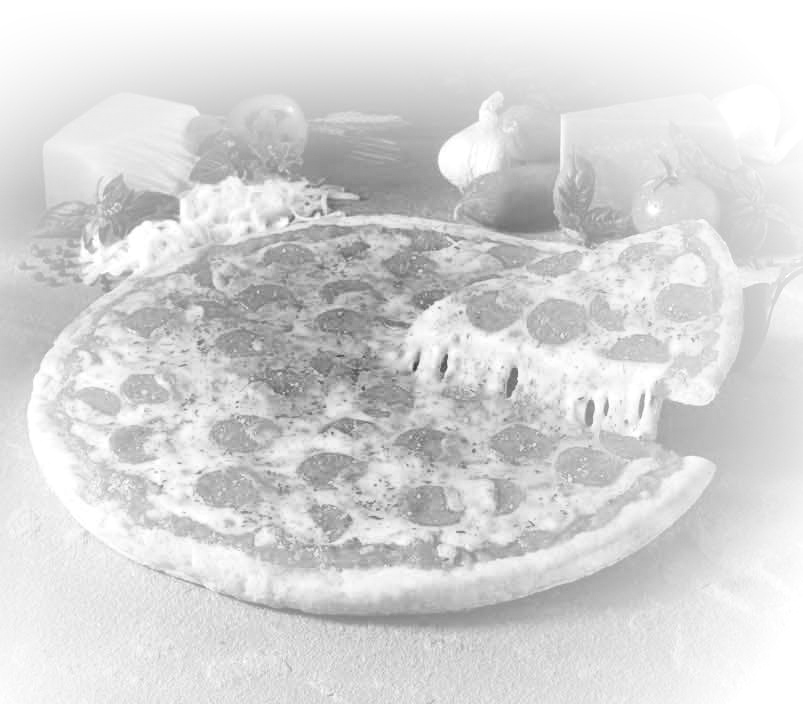
\includegraphics[width=.45\textwidth]{img/barao/pizza.jpg}
\end{figure}

\subsubsection*{Alguns telefones:}

\begin{itemize}
    \item   \textbf{Restaurante Baronesa}
        \\Telefone: (19) 3289-9087
        \\Endereço: Rua Benedito Alves Aranha, 44
        \\Site: \url{restaurantebaronesa.com.br}

    \item   \textbf{China In Box} (Faz entrega em Barão)
        \\Telefone: (19) 3254-5601
        \\Endereço: Rua Romualdo Andreazzi, 333

    \item   \textbf{TBONE Steak Bar}
        \\Telefone: (19) 3289-0485
        \\Endereço: Rua Maria Tereza Dias da Silva, 700

    \item   \textbf{Ginza Bar}
        \\Telefone: (19) 3289-9281
        \\Endereço: Rua Roxo Moreira, 1768

    \item   \textbf{Bardana}
        \\Telefone: (19) 3289-9073
        \\Endereço: Av. Dr. Romeu Tortima, 1500

    \item   \textbf{Terraço}
        \\Telefone: (19) 3289-7920
        \\Endereço: Rua Roxo Moreira, 1344

    \item   \textbf{Pastelaria Oba-Oba}
        \\Telefone: (19) 3249-1908
        \\Endereço: Rua Benedito Alves Aranha, 115

    \item   \textbf{Estância Grill}
        \\Telefone: (19) 3289-1511
        \\Endereço: Av. Albino J. B. de Oliveira, 271
        
    \item   \textbf{Pizza Mais}
        \\Telefone: (19) 3289-0320 / (19) 3289-2754

    \item   \textbf{Barão das Pizzas}
        \\Telefone: (19) 3249-1630
        \\Endereço: Rua Jerônimo Pattaro, 351

    \item   \textbf{Pizza Fiori}
        \\Telefone: (19) 3289-3514
        \\Endereço: Av. Santa Isabel, 405

    \item   \textbf{Ki-Pizza}
        \\Telefone: (19) 3289-0863
        \\Endereço: Rua Horácio Leonardi, 76

    \item   \textbf{Super Mega Pizza}
        \\Endereço: Rua Francisca Resende Merciai, 125B
        \\Telefone: (19) 3288-0606 / (19) 3288-0608
        \\Site: \url{supermegapizza.com}

    \item   \textbf{NADOG'S -- Hot Dog do Nado}
        \\Telefone: (19) 3029-2270

    \item   \textbf{Casa da Moqueca} (prato mais caro, mas serve duas pessoas)
        \\Telefone: (19) 3289-3131
    
% \end{itemize}

% \subsection{E à noite?}

% \begin{itemize}
    \item   \textbf{Hot-dog Independência:}
        \\Telefone: (19) 3289-8805
        \\Endereço: Rua Angela Signol Grigol, 742
        \\\\
        Tem vários tipos de hot-dogs (com catupiry, com cheddar, com frango
        {\dots}) e tem preços menores que os do Rod Burguers. O único problema é
        que eles cobram taxa de entrega para um lanche e fecham à meia-noite.

    \item   \textbf{Kalunga Lanches:}
        \\Telefone: (19) 3289-5236
        \\Endereço: Rua Sebastião Bonomi, 40
        \\\\
        Perto da moradia, eles não entregam, mas ficam abertos até altas horas.
        Destaque para o caldinho de feijão. Obs: o lugar é limpo e bom.

    \item   \textbf{Barão Hamburgueria:}
        \\Telefone: (19) 3289-9753
        \\Endereço: Av. Albino J. B. de Oliveira, 476
        \\\\
        Rua Localizada na entrada de Barão Geraldo servem lanches parecidos com
        os do Mega Sandubão, lá eles dão outro tipo de maionese e em geral os
        preços são tão caros quanto do Mega Sandubão. Também entregam até meia
        noite.

    \item   \textbf{Lanchão \& Cia:}
        \\Telefone: (19) 3289-3665
        \\Endereço: Av. Albino J. B. de Oliveira, 1214
        \\Site: \url{lanchaoecia.com.br}
        \\\\
        Um dos melhores lanches de Campinas (quiçá o melhor). Os lanches
        geralmente são grandes e muito bons, e os preços são compatíveis com a
        qualidade e quantidade. Eles servem no carro se você preferir, com uma
        bandeja que fica presa no vidro. Fica no centro de Barão Geraldo,
        proximo ao Santander e Pão de Açúcar. Destaque para a batata frita,
        feita de uma forma muito diferente, extremamente crocante e quase
        cremosa por dentro.

    \item   \textbf{Burger King:}
        \\Endereço: Av. Albino J. B. de Oliveira, 1000
        \\\\
        Aberto das 10h às 22h

    \item   \textbf{Ponto 1:}
        \\Telefone: (19) 3289-2378
        \\Endereço: Rua Eduardo Modesto, 54
        \\Site: \url{ponto1bar.com}

      \item \textbf{Sapore Pizza:}
        \\Telefone: (19) 3289-0228
        \\Endereço: Av. Santa Isabel, 326
        \\\\
        Para quando você estiver com pelo menos mais um amigo para rachar a
        pizza, acaba sendo uma boa pedida. Geralmente as pizzas de mussarela e
        de calabreza estão com preços bem acessíveis. Além de pizzas, eles fazem
        esfihas e batate rechada.Eles entregam até 23h.

        A Sapore também tem self-service no almoço, R\$ 15,50 por pessoa durante
        a semana e um pouco mais aos fins de semana, e marmita pra retirar no
        local, R\$ 36 o quilo pra você montar sua marmita com as coisas do
        self-service, ou R\$ 11 a marmita pronta, há várias opções de carnes.

    \item   \textbf{McDonald's:}
        \\Telefone: (19) 3289-0318
        \\Endereço: Av. Albino J. B. de Oliveira, 1430
        \\\\
        Dispensa apresentações. Entregas das 11h às 23h. Costuma ficar aberto de
        madrugada, até as 4 da manhã.

    \item   \textbf{Barraquinhas:}
        \\Há várias barraquinhas de hot-dog no centro de Barão e perto da
        moradia. Destaque para o dog do terminal, o Hot Dog Central, o Pedrogue
        e o dogão da moradia. Se você quiser um lanche, uma boa pedida é o Star
        Tresh (Raimundão ou Guarujá, chame como você quiser), que fica perto do
        balão da Avenida 2 e costuma ficar aberto até altas horas. Perto da
        Unicamp, ao lado do posto Ipiranga que fica na avenida 1 também tem um
        dog prensado muito bom e barato.
\end{itemize}

\subsection{Marmitex}

Entrega em casa. Bom e barato.

\begin{itemize}
    \item   \textbf{Tia Rita}
        \\Telefone: (19) 3249-2899

    \item   \textbf{Hailton}
        \\Telefone: (19) 3249-0153
\end{itemize}

Obs: A Sapore Pizza também entrega Marmitex.

\begin{figure}[h!]
    \centering
    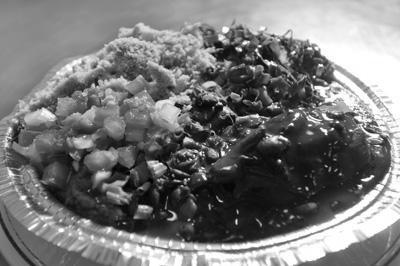
\includegraphics[width=.45\textwidth]{img/barao/marmitex.jpg}
\end{figure}

\subsection{Bares, lanchonetes e restaurantes}

\begin{itemize}
    \item   \textbf{Açaizeiro Brasil:} Serve um açaí muito bom e vários tipos de
        comidas mais leves, como lanches naturais, crepes e saladas, além de
        vários sucos. O preço não é caro e a comida é boa.
        \\Endereço: Av. Santa Isabel, 518
        \\Telefone: (19) 3365-6555 %TODO: verificar número

    \item   \textbf{Aulus VideoBar \& Restaurant:} A comida é muito boa, porém
        cara, especialmente no final de semana. A exceção fica no preço do
        marmitex, apenas R\$ 12,50. O ambiente do restaurante é muito diferenciado,
        com bicicletas e ferroramas no teto, por exemplo.
        \\Endereço: Av. Prof. Atílio Martini, 939
        \\Telefone: (19) 3289-4453
        \\Site: \url{aulus.com.br}

    \item   \textbf{Bagdá Café -- Bar \& Esfiharia:} Esfihas boas, mas um pouco
        caras. Entregam em Barão (cardápio no site), mas em horários de pico
        costumam demorar um pouco. A música ambiente inclui música ao vivo e
        ritmos variados, desde a MPB ao Blues.
        \\Endereço: Av. Santa Isabel, 233
        \\Telefone: (19) 3289-0541 / (19) 3289-1842
        \\Site: \url{bagdacafe.com.br}

\begin{figure}[h!]
    \centering
    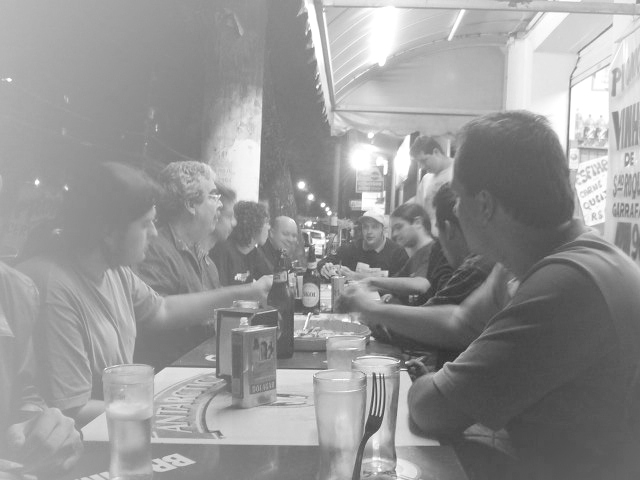
\includegraphics[width=.45\textwidth]{img/barao/bar.jpg}
\end{figure}

    \item   \textbf{Bar do Coxinha:} Famoso pela coxinha (realmente boa), vale a
        pena ir lá, mas é relativamente caro. Localiza-se perto da avenida Santa
        Isabel, na rua da Sapore Pizza.

    \item   \textbf{Bar do Jair:} Outro lugar famoso pela coxinha: só que esta é
        de carne seca. Fica relativamente perto da Moradia.
        \\Endereço: Rua Eduardo Modesto, 212

    \item   \textbf{Barão da picanha:} Churrascaria rodízio localizada na
        avenida Albino José Barbosa de Oliveira, logo na entrada de Barão.

    \item   \textbf{Batataria Suiça:} Do lado do Mega Sandubão, serve batatas
        recheadas bem diferentes. É um pouco caro, mas vale a pena conferir. Uma
        dica é que às terças-feiras você compra uma batata, mas recebe duas.
        \\Endereço: Estrada da Rhodia -- Praça José Geraldi, a 50m do posto Esso
        \\Telefone: (19) 3201-1174
        \\Site: \url{battataria.com.br}

    \item   \textbf{Boi Falô:} O restaurante é um rancho, com comida típica do
        interior. É excelente, mas um pouco caro (cerca de R\$30,00 por pessoa),
        um lugar perfeito para levar seus pais quando eles vêm te visitar (e
        pagam o almoço!). Abre apenas nos almoços de sábado e domingo.
        \\Endereço: Rua do Sol, 600
        \\Telefone: (19) 3289-6671 / (19) 3287-6342%TODO: verificar número

    \item   \textbf{Cachaçaria Água Doce:} Localizada na avenida 1, é um lugar
        frequentado por pessoas mais velhas, ótimo para comida e bebida (pinga,
        especialmente), mas é bem caro.

    \item   \textbf{Casa São Jorge:} Música ao vivo todas as noites, com boa
        variedade. Localiza-se na rua Santa Isabel, mais ou menos perto da
        moradia.

    \item   \textbf{Empório Nono:} Caro, tem um chopp muito bem tirado e os
        melhores petiscos de Campinas. Localiza-se na avenida Albino José
        Barbosa de Oliveira, quase em frente ao terminal.

    \item   \textbf{Estância Grill:} Logo na entrada de Barão. Tem rodízios de
        carne e de pizza à noite.
        \\Endereço: Av. Albino J. B. de Oliveira, 271
        \\Site: \url{www.estanciacampinas.com.br}
        \\Telefone: (19) 3289-8697 / (19) 3289-6055 / (19) 3289-1511

    \item   \textbf{Fernando's:} No centro de Barão, perto do Banespa, serve
        cerveja e lanches baratos e muito bons principalmente porque vêm
        acompanhados de uma porção pequena de fritas! Um lugar simples mas muito
        limpo e agradável principalmente em relação ao atendimento. Fecha as 23h
        se segunda a quinta e sábado, tem música ao vivo na sexta e por enquando
        ainda não abre nos domingos.

    \item   \textbf{Fran's Café:} Cafeteria. Vende lanches, cafés, doces,
        salgados e bebidas (quentes ou geladas). Fazem também cafés da manhã.
        Mas é um pouco caro.
        \\Endereço: Av. Albino J. B. de Oliveira, 1600 

    \item   \textbf{Greg Burguers:} Uma lanchonete muito boa, mas também muito
        cara.  Uma das especialidades lá é o milk-shake (realmente muito bom).
        Fica na estrada da Rhodia (na esquina da Paneteria Di Capri). Só
        funciona à noite, de terça a domingo.
        \\Endereço: Rua Maria Tereza Dias da Silva, 664
        \\Telefone: (19) 3289-6400
        \\Site: \url{gregburgers.com.br}
\end{itemize}

\begin{figure}[h!]
    \centering
    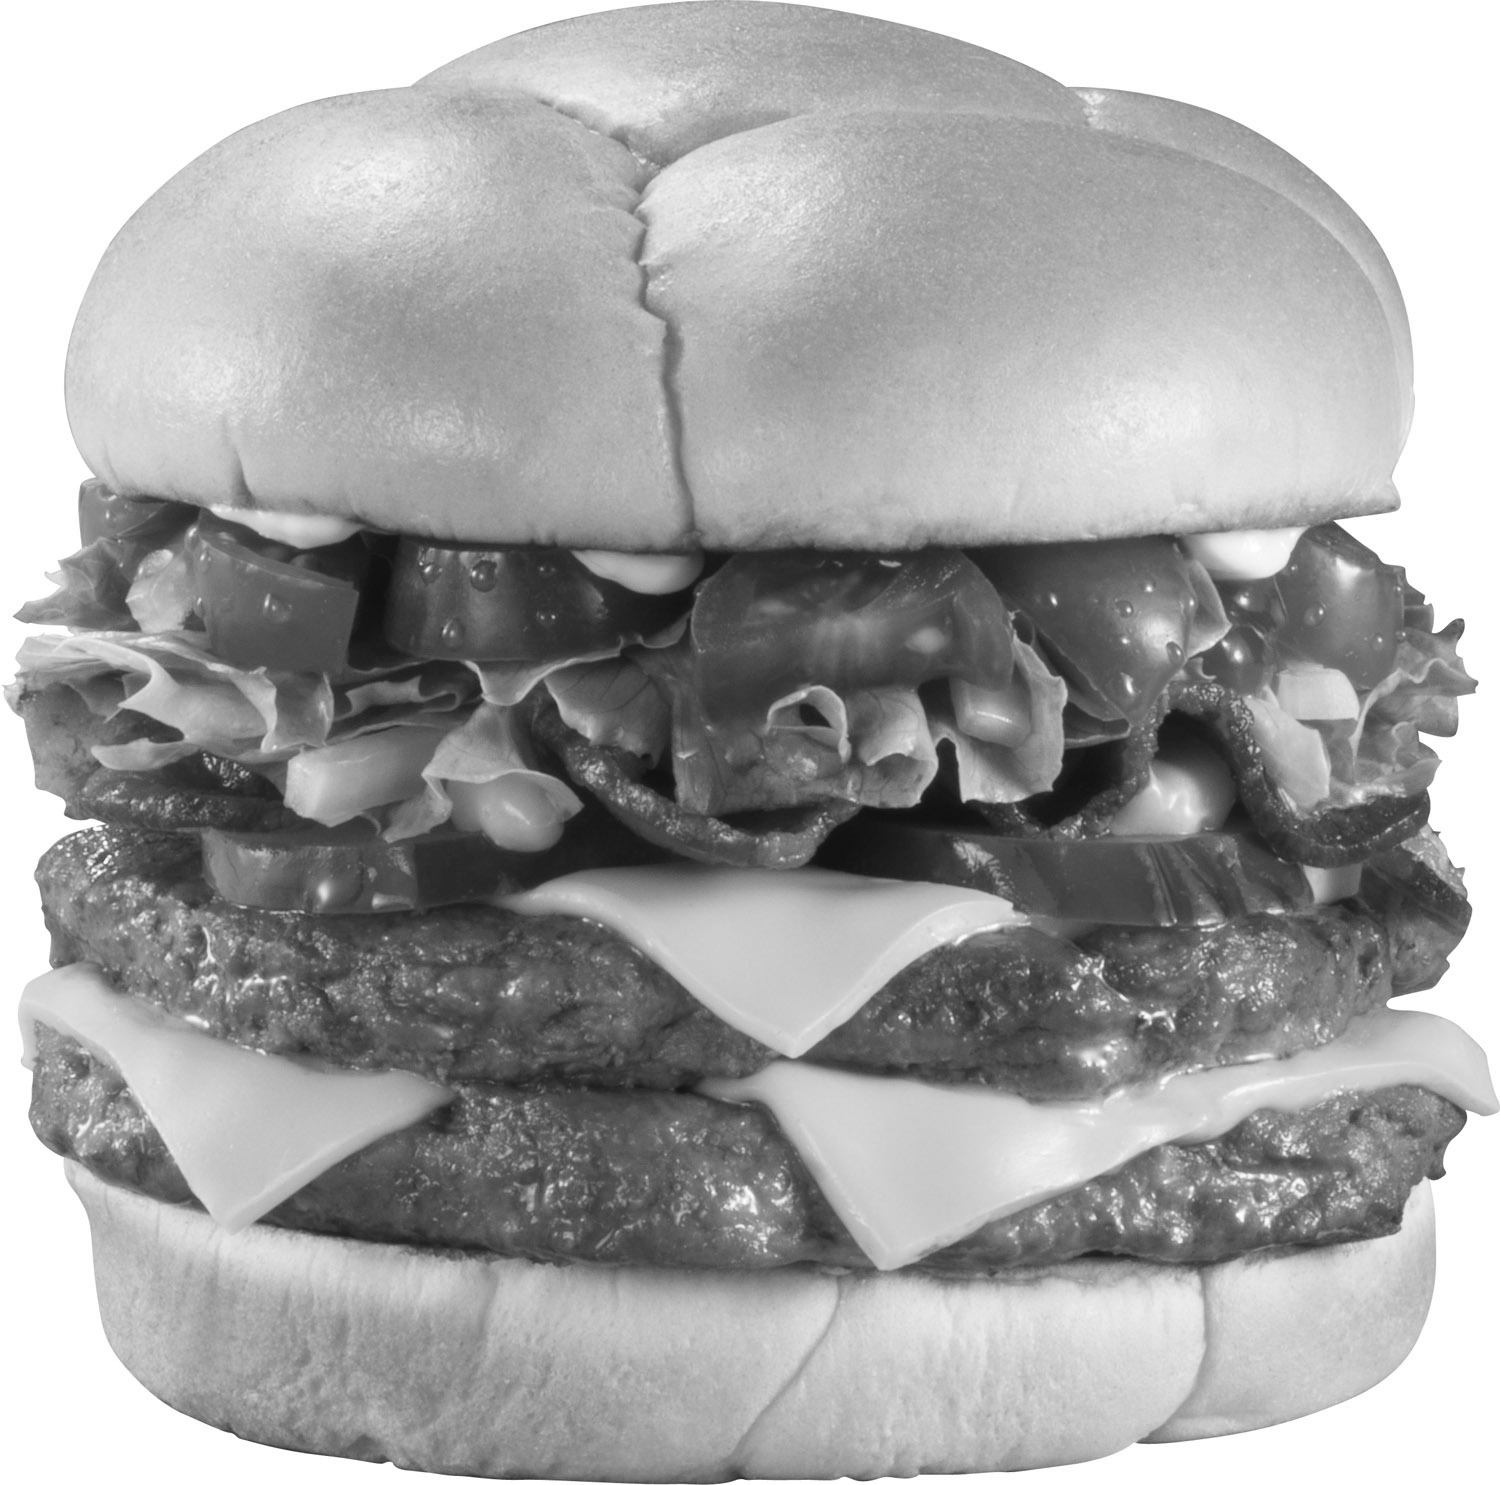
\includegraphics[width=.45\textwidth]{img/barao/burger.jpg}
\end{figure}

\begin{itemize}
    \item   \textbf{La Salamandra:} Restaurante mexicano, localizado na Av. 2,
        perto do Yaki-Ten. Comida boa e preço compatível. Tabém é um ótimo lugar
        para se levar os pais quando eles vêm visitar.
        \\Endereço: Av. Prof. Atílio Martini, 152
        \\Telefone: (19) 3289-2011

    \item   \textbf{Makis Place:} Temakeria próxima ao terminal.
        \\Endereço: Av. Albino J. B. de Oliveira, 976
        \\Telefone: (19) 3367-3077
        \\Site: \url{makis.com.br}

    \item   \textbf{Mega Sandubão:} 
        Antigo Ponto Final. Lanchonete localizada na estrada da Rhodia e entrega
        lanches até a meia noite. Muitos gostam bastante dessa lanchonete pela
        famosa maionese temperada que eles servem, não se esqueça de pedir
        quando for comprar lanches.À noite serve, cerveja a um bom preço. Localiza-se
        na estrada da rhodia (continuação da avenida Albino José de Oliveira).
        \\Endereço: Av. Albino J. B. de Oliveira, 2287
        \\Telefone: (19) 3288-0204

    \item   \textbf{Quintal do Neto:} No alto da avenida 1, perto do balão de
        entrada em barão geraldo, tem cerveja a preços razoáveis, salgados
        (coxinha e quibe) grandes, e mesas de sinuca (de ficha e por hora).
        \\Endereço: Av. Dr Romeu Tórtima, 104

    \item   \textbf{Rudá:} Localizado na Santa Isabel, bar com música ambiente.

    \item   \textbf{Solar dos Pampas:} Buffet excelente. Custa R\$ 24,00 apenas
        a comida e R\$ 34,00 com refrigerante e suco incluídos (o tanto que você
        conseguir beber). Fazem um esquema no aniversário das pessoas que sai
        por R\$ 18,00 com rodízio, cerveja, refrigerante, buffet, sorvete e
        pinga à vontade. Ao lado do Estância d'Oliveira.
        \\Endereço: Av. Dr. Romeu Tortima, 165
        \\Telefone: (19) 3289-1484 / (19) 3289-7869
        \\Site: \url{www.solardospampasbarao.com.br}

    \item   \textbf{Star Clean:} É o bar mais próximo à Unicamp, e por isso está
        sempre cheio. Principal ponto de encontro depois da aula e tem um bom
        preço.

    \item   \textbf{Subway:} Lanchonete. Vende dos mais variados tipos de
        lanches.  Lanches muito bons, e não tão caros. Localiza-se no Tilli
        Center (avenida Albino José Barbosa de Oliveira, 1556, esquina com a
        avenida 2). Do lado do Subway tem um caixa 24 horas que trabalha com os
        principais bancos. O Subway faz entregas em algumas regiões de Barão.
        \\Telefone: (19) 3201-8411 / (19) 3201-8410
        \\Site: \url{subdelivery.com.br}

      \item \textbf{Temakeria Barão Geraldo:} Lugar relativamente novo, meio
        caro. Vende só temaki e bebidas. O horário de funcionamento é bastante
        conveniente.  
        \\Endereço: Av. Dr. Romeu Tortima, 1259 
        \\Telefone: (19) 3289-0802 
        \\Horário de funcionamento: domingo a terça das 11h30 às 0h, quarta a
        sábado das 11h30 às 6h 
        \\Site: \url{tmkr.com.br}

    \item   \textbf{Estância d'Oliveira:} Antigo Universo das Massas. Rodízio de
        massas perto do Terminal. Bom e não é caro. De domingo à noite é o
        horário mais barato e dá pra encher bem o bucho de massa. Depois de ir
        até lá, você não vai querer saber de comer massas por um bom tempo.
        \\Endereço: Av. Albino J. B. de Oliveira, 576
        \\Telefone: (19) 3289-5369 

    \item   \textbf{Vila Ré - Pizza:} Pizzaria próxima do terminal e do
        supermercado Dalben. Tem alguns sabores diferentes, as pizzas são boas e
        o preço não é alto. Possui serviço de entrega das 18h às 23h.
        \\Endereço: Av. Albino J. B. de Oliveira, 658
        \\Telefone: (19) 3289-0321

    \item   \textbf{Bar do Zé:} O pub tem apresentações ao vivo todas as
        semanas.  Localiza-se também na avenida Albino José de Oliveira, bem em
        frente ao Pão de Açúcar.
        \\Site: \url{obardoze.com.br}
        \\Telefone: (19) 3289 3159

    \item   \textbf{Echos Studio Bar:} Um bar relativamente novo, possui
        apresentaçes ao vivo direto, que costumam ser de Rock, Blues ou Jazz.
        Fica entre a Santa Isabel e Albino J. B. de Oliveira.
        \\Endereço: Rua Agostinha Pátaro, 54
        \\Site: \url{echo.mus.br/studiobar}
        \\Telefone: (19) 3201-8900

    \item   \textbf{Marambar:} Possui bebidas, lanches, sucos e porções a preços
        razoáveis. Ambiente agradável, ao ar livre, muito próximo da Unicamp.
        Bastante frequentado por computeiros e engenheiros em geral, além de
        muita gente de outros cursos. Funciona de segunda a sexta, das 7h30 até
        as 2h30, e aos sábados, das 9h até a 1h.
        \\Endereço: Av. Dr. Romeu Tortima, 1538 (próximo ao balão da avenida 1)
        
\end{itemize}

\newpage
%%%%% Diversão
% Este arquivo .tex será incluído no arquivo .tex principal. Não é preciso
% declarar nenhum cabeçalho

\section{Diversão}
Está com vontade de fazer algo para livrar a cabeça do stress da vida acadêmica?
Como em toda universidade, na Unicamp existem inúmeras opções de entretenimento
e diversão, desde festas e bares até cinemas e teatros.

Se você gosta ou se interessa por jogos de tabuleiro, a dica é a luderia que
existe na 2, o Metropoly. Lá você paga 12 reais por pessoa e joga a vontade. A
comida e bebida são um pouco caras, mas mesmo assim compensa. Se você não sabe o
que jogar, peça sugestões aos garçons de jogos.

O cinema mais próximo e mais conveniente é o do Shopping Dom Pedro. Estudantes
pagam meia da meia na segunda feira, então é uma ótima opção para quem quer se
divertir sem gastar muito dinheiro.

Se você curte festas e baladas, fique atent* na saída do bandeco, pois é lá que
elas são divulgadas. A maioria das festas acontecem às quintas feiras em
repúblicas ou no Campinas Hall. Existem também festas dentro da Unicamp, que
apesar de serem proibidas, acontecem com certa regularidade.

\subsection{Espaços culturais}

\begin{itemize}
    \item   \textbf{Casa do Lago:} Dentro da Unicamp, mantém uma programação
        quase diária de cinema e exposições. Este ano estão viabilizando a
        instalação de café e revistaria. A página da casa do lago é:
        \\\url{www.preac.rei.unicamp.br/casadolago}

    \item   \textbf{Semente:} Fica no fim da avenida Santa Isabel, depois da
        moradia. Sempre tem apresentações artísticas, como teatros e espetáculos
        musicais.
\end{itemize}

\subsection{Cinemas}

\begin{itemize}
    \item   \textbf{Kinoplex}
        \\Endereço: Shopping D. Pedro (Rodovia Dom Pedro I, Km 137 -- Jd. Sta. Genebra)
        \\Telefone: (19) 3131-2800
        \\Site: \url{kinoplex.com.br}

    \item   \textbf{Cinemark Iguatemi}
        \\Endereço: Shopping Center Iguatemi (Av. Iguatemi, 777 -- Vila Brandina)
        \\Site: \url{cinemark.com.br}

    \item   \textbf{Box Cinépolis Campinas}
        \\Endereço: Campinas Shopping (Rua Jacy T. de Camargo, 940 -- Jardim do Lago)
        \\Telefone: (19) 3268-2288
        \\Site: \url{cinepolis.com.br}

    \item   \textbf{Cine Galleria}
        \\Endereço: Galleria Shopping (Rod. Dom Pedro I, Km, 131,5 -- Jd. Nilópolis)
        \\Telefone: (19) 3207-1333
        \\Site: \url{www.iguatemi.com.br/galeriashopping/cinema/}

    \item   \textbf{Cine Moviecom Unimart}
        \\Endereço: Shopping Unimart (Av. John Boyd Dunlop, 350 -- Chácara da República)
        \\Telefone: (19) 3744-4791
        \\Site: \url{moviecom.com.br}

    \item   \textbf{Multiplex Parque das Bandeiras}
        \\Endereço: Shopping Parque das Bandeiras (Av. John Boyd Dunlop, 3900)
        \\Telefone: (19) 3227-1869
        \\Site: \url{www.cinearaujo.com.br}
		
    \item   \textbf{Topázio Cinemas}
        \\Endereço: Shopping Prado (Av. Washington Luís, 2480 -- Parque Prado)
        \\Telefone: (19) 3276-3610
        \\Site: \url{www.shoppingprado.com.br/web/cinema/}

    \item   \textbf{Cinesercla Spazio Ouro Verde}
        \\Endereço: Shopping Spazio Ouro Verde
        \\Telefone: (19) 3726-2110
        \\Site: \url{www.cinesercla.com.br/cinemas/detalhes/cinesercla_spazio_ouro_verde}

\end{itemize}

\subsection{Teatros}

\begin{itemize}
    \item   \textbf{Lume Teatro}
        \\Endereço:  Rua Carlos Diniz Leitão, 150 Vila Santa Isabel -- Barão Geraldo
        \\Telefone: (19) 3289-9869
        \\Site: \url{lumeteatro.com.br}

    \item   \textbf{Teatro Interno Luiz Otávio Burnier}
        \\Endereço: Centro de Convivência Cultural (Praça Imprensa Fluminense s/nº -- Cambuí)
        \\Telefone: (19) 3232-5977 % Ninguem atendeu - Ligar novamente

    \item   \textbf{Teatro de Arena}
        \\Endereço: Centro de Convivência Cultural (Praça Imprensa Fluminense s/nº -- Cambuí)
        \\Telefone: (19) 3232-5977 % Ninguem atendeu - Ligar novamente

    \item   \textbf{Teatro Carlos Maia}
        \\Endereço: Rua Cel. Quirino, 2 -- Bosque dos Jequitibás
        \\Telefone: (19) 3231-8795
        \\Site: \url{bit.ly/1muLXRz}

    \item   \textbf{Teatro José de Castro Mendes}
        \\Endereço: Praça Corrêa de Lemos, s/nº -- Vila Industrial
        \\Telefone: (19) 3272-9359
        \\Site: \url{bit.ly/1AHgZKw}

    \item   \textbf{Auditório Beethoven (Concha Acústica)}
        \\Endereço: Av. Heitor Penteado, s/nº -- Portão 2 -- Lagoa do Taquaral
        \\Site: \url{bit.ly/1tPxFyT}

    \item   \textbf{Teatro de Arte e Ofício}
        \\Endereço: Rua Conselheiro Antônio Prado, 529 -- Vila Nova
        \\Telefone: (19) 3241-7217 / (19) 98200-0149
        \\Site: \url{bit.ly/1xT55Lg}

    \item   \textbf{Teatro Dom Nery (Externato São João)}
        \\Endereço: Rua José de Alencar, 360  Centro
        \\Telefone: (19) 3231-2644  % Ninguem atendeu - Ligar novamente
        \\Site: \url{bit.ly/1xH9Qsy}

     \item   \textbf{Teatro Teresa Aguiar (Conservatório)}
         \\Endereço: Rua José de Alencar, 701 -- Centro
    %     \\Telefone: (19) 3232-9345 -  Numero nao existe

    \item   \textbf{Teatro da Vila Padre Anchieta}
        \\Endereço: Av. Cardeal Dom Agnelo Rossi, s/nº -- Vila Padre Anchieta
        \\Telefone: (19) 3282-0024 / (19) 3781-0382 % Ninguem atendeu - Ligar novamente
                    % Atendeu mas ficou mudo - Tentar novamente
        \\Site: \url{bit.ly/1DnEsTg}

     \item   \textbf{Centro Cultural Evolução}
         \\Endereço: Rua Regente Feijó, 1087 -- Centro
    %     \\Telefone: (19) 3232-9959 - Numero nao existe

    \item   \textbf{Teatro Amil (Antigo Teatro TIM)}
        \\Endereço: Shopping D. Pedro, Entrada das flores
        \\Telefone: (19) 3756-9890 / (19) 3756-9891
        \\Site: \url{bit.ly/143BpQH}

    \item   \textbf{Teatro Brasil Kirin}
		\\Endereço: Shopping Iguatemi (Av. Iguatemi, 777 -- Vila Brandina).
		\\Telefone: (19) 3294-3166
		\\Site: \url{www.teatrobrasilkirin.com.br}

    \item   \textbf{Teatro do SESC}
		\\Endereço: Rua Dom José I, 270 -- Bonfim (próximo à rodoviária nova)
		\\Telefone: (19) 3737-1500

    \item   \textbf{Teatro do SESI Amoreiras}
		\\Endereço: Av. das Amoreiras, 450 -- Parque Itália.
		\\Telefone: (19) 3272-3560 % Fora de servico - tentar novamente

    \item   \textbf{Teatro SOTAC}
		\\Endereço: Rua Barão de Jaguara, 2 -- Bosque
		\\Telefone: (19) 3235-2266
		\\Site: \url{www.sotac.com.br}

    \item   \textbf{Teatro Sia Santa}
		\\Endereço: Rua Sebastião Paulino dos Santos, 20 -- Parque Santa Bárbara
        \\Telefone: (19) 3281-3174 / (19) 3281-3306
		\\Site: \url{www.siasanta.art.br}
\end{itemize}

\subsection{Boates e baladas}

\begin{figure}[h!]
    \centering
    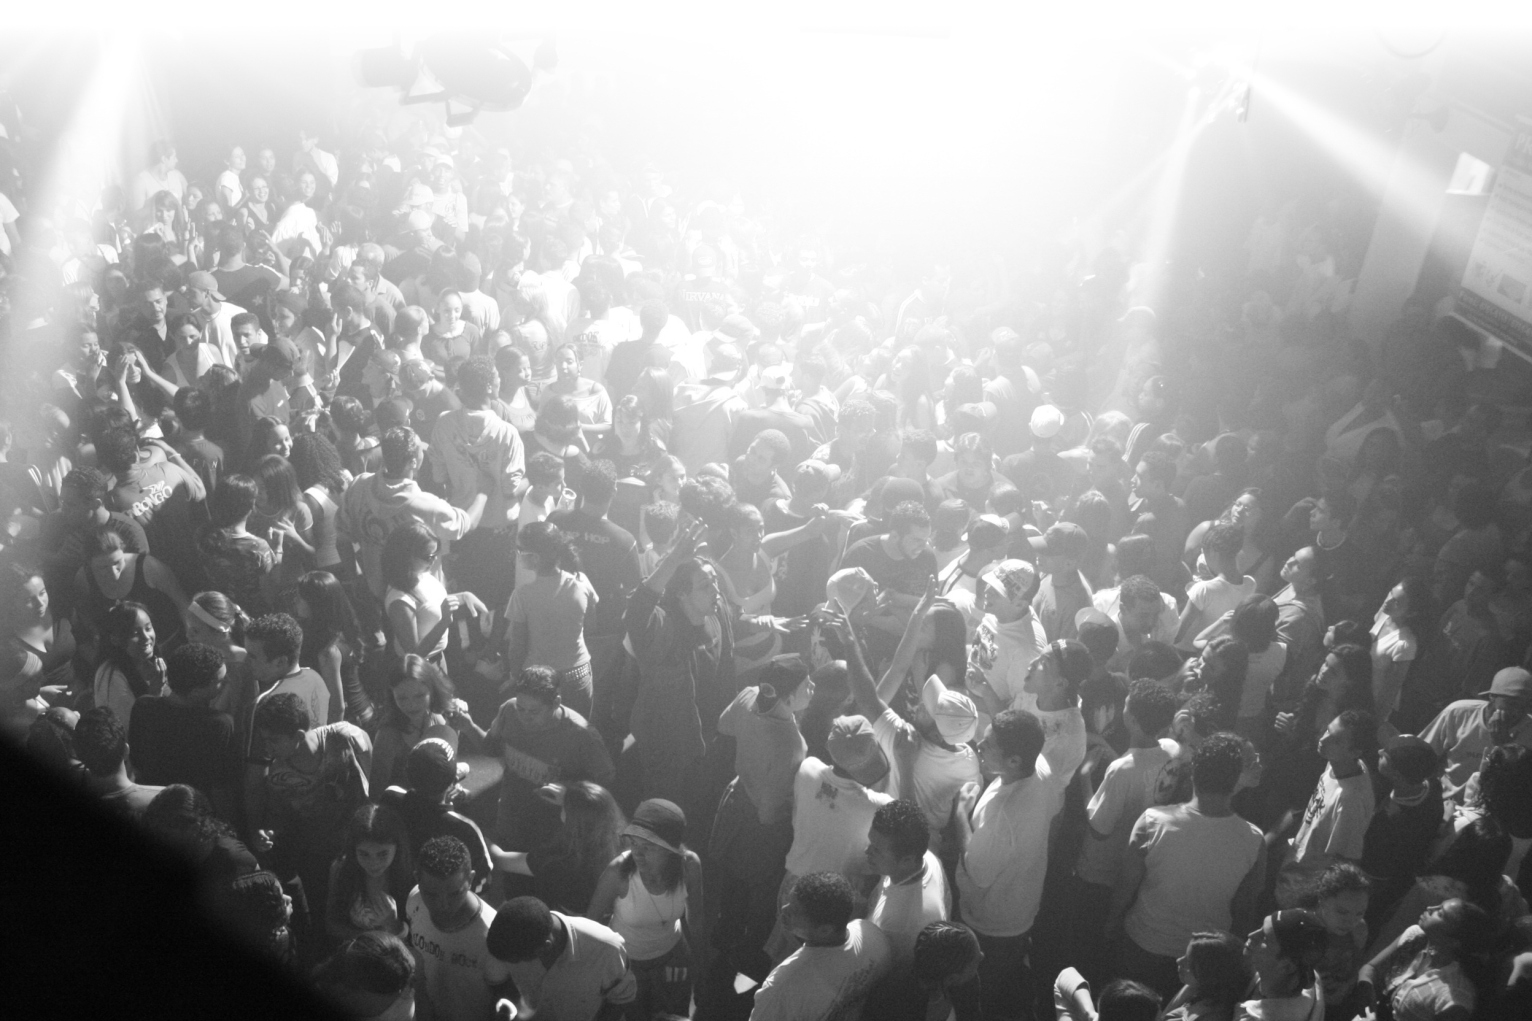
\includegraphics[width=.45\textwidth]{img/barao/boate.jpg}
\end{figure}

\begin{itemize}
    \item   \textbf{Cooperativa Brasil:} Para quem gosta de um bom forró, sempre
        com shows diversos. A galera gosta muito da quarta-universitária.
        \\Site: \url{cooperativabrasil.com.br}

    \item   \textbf{Campinas Hall:} Muitas das festas mais legais da Unicamp
        acontecem lá (como a Festa Brega e a Festa do Contrário), perto da PUCC.
        É bem grande.

    \item   \textbf{Barril da Máfia:} Programação musical bem variada e um clima
        bem legal.
        \\Site: \url{barrildamafia.com.br}

    \item   \textbf{Kraft:} Localizada próxima ao Taquaral (na Avenida
        Imperatriz Leopoldina), toca musica psi a noite toda e fica aberta até
        quase o amanhecer. Mulher entra de graça até a meia-noite.

    \item   \textbf{Cambuí:} Neste bairro existem diversos barzinhos, a maioria
        é temático, alguns são um pouco caros e cobram covert. É um ótima
        escolha para quem tiver carro pois fica um pouco longe de Barão.
\end{itemize}

\subsection{Shopping Centers}

\begin{figure}[h!]
    \centering
    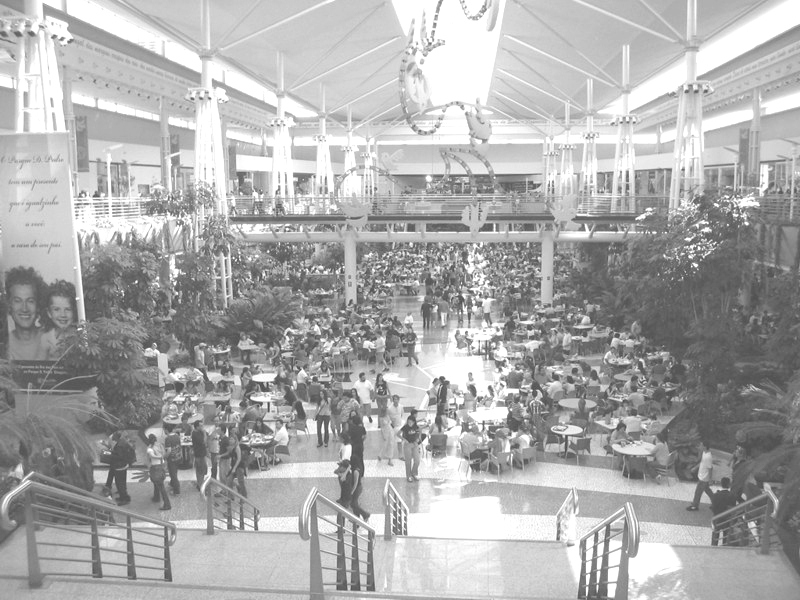
\includegraphics[width=.45\textwidth]{img/barao/d_pedro.jpg}
\end{figure}

\begin{itemize}
    \item   \textbf{Shopping Parque D. Pedro:} Foi considerado o maior shopping
        da América Latina até pouco tempo atrás. Localiza-se na Rodovia Dom
        Pedro, km 137 (razoavelmente próximo à Unicamp). O ônibus 3.38, que sai
        do Terminal Barão, vai para lá e para o Iguatemi. Outras opções de
        ônibus saindo do terminal são 2.10 e 3.00.
        \\Site: \url{parquedpedro.com.br}

    \item   \textbf{Shopping Iguatemi:} Shopping normal, o mais antigo e o
        segundo maior de Campinas. Localiza-se na Avenida Iguatemi, 777. O 3.38
        demora uns 40 minutos para chegar lá. Frequentado pela galera mais nova
        e pelo pessoal com um pouco mais de dinheiro.
        \\Site: \url{www.iguatemicampinas.com.br}

    \item   \textbf{Parque das Bandeiras Shopping:} Inaugurado no fim de 2012.
        Localiza-se na região do Campo Grande, região noroeste de Campinas 
        (MUITO longe). Conta com telas de cinema de 300 m$^{2}$.
        \\Site: \url{shoppingparquedasbandeiras.com.br}

    \item   \textbf{Shopping Jaraguá:} Shopping pequeno. Localizado na Rua Conceiçao, 
         230, no Centro de Campinas. O ônibus 3.30, no sentido Terminal Central -- Unicamp,
         para razoavelmente próximo a ele. Até 2009 existia uma outra unidade na 
         Avenida Brasil.

    \item   \textbf{Campinas Shopping:} Longe a dar com pau, mas as lojas não
        são muito caras. Localiza-se no Jardim do Lago, às margens das rodovias 
        Anhanguera e Santos Dumont. Provavelmente você nunca irá lá.
        \\Site: \url{campinasshopping.com.br}

    \item   \textbf{Shopping Prado:} Shopping pequeno, porém as lojas são um 
        pouco caras. É outro que fica muito longe e que você provavelmente nunca 
        irá até lá. Localizado na Av. Washington Luís, 2480 -- Parque Prado.
        \\Site: \url{pradoboulevard.com.br}

    \item   \textbf{Galleria Shopping:} Muito bonito, mas lojas muito caras.
        Também localizado na Rodovia Dom Pedro, mas no km 131,5. O ônibus 3.00
        sai do terminal de Barão Geraldo e passa lá.
        \\Site: \url{www.galleria.com.br}

    \item   \textbf{Shopping Unimart:} Shopping pequeno, as lojas não são muito
        caras. Localiza-se na Avenida John Boyd Dunlop, 350. O ônibus 1.34 sai
        do terminal de Barão Geraldo e passa próximo.
        \\Site: \url{unimart.com.br}
    
    \item   \textbf{Shopping Spazio Ouro Verde:} Shopping pequeno, inaugurado 
        no fim de 2010. As lojas não são muito caras. É outro Shopping que 
        também fica MUITO longe. Localiza-se na Av. Ruy Rodriguez, 3900, 
        Parque Universitário (região do Ouro Verde).
        \\Site: \url{spazioouroverde.com.br}

    \item   \textbf{Ventura Mall:} Shopping pequeno, porém as lojas são muito caras.
        Fica localizado na Av. Moraes Salles, 2790 -- Nova Campinas.
        \\Site: \url{venturamall.com.br}
\end{itemize}

\newpage
%%%%% Transporte
% Não é preciso declarar nenhum cabeçalho

\section{Transporte}
\subsection{Voltar para casa}

Para os calouros de fora de Campinas, além de escolher a nova morada é
importante reunir informações sobre como realizar o trajeto entre sua cidade e
Campinas.

A forma usual é ir de ônibus, mas tenha em mente que a rodoviária é longe e os
trajetos de ônibus até lá são demorados. O endereço da rodoviária é: Rua Pereira
Lima, s/n. Há duas linhas que passam por lá: o 332 (que passa dentro da Unicamp)
para dentro da rodoviária, mas demora mais pra chegar que o 331, que sai do
terminal e para do lado de fora da rodoviária. Em horários de pico, o trajeto
pode demorar quase uma hora, então cuidado para não perder o horário do ônibus
para sua cidade. Também não se esqueça de portar algum cartão para andar nos
ônibus de Campinas, seja o Bilhete Único ou um dos dois cartões avulsos (Bilhete
1 Viagem e Bilhete 2 Viagens). Caso contrário, não será possível embarcar em um
ônibus.

Os que vêm de mais longe certamente farão uso do aeroporto de Viracopos, cujo
telefone é 3725-5000. Para chegar ao aeroporto existe a linha 193 que sai da
rodoviária e vai para o aeroporto, e também faz o trajeto de volta. Porém, ir
com ônibus circular pode ser um transtorno quando estiver com muita bagagem. Uma
outra alternativa é a Lirabus que também faz o traslado da rodoviária para o
aeroporto. A passagem da Lirabus custa R\$9,00 (R\$9,80 se sair da Rodoviária,
pois paga taxa de embarque) e os horários podem ser conferidos no site
\url{www.lirabus.com.br/}.

Para quem for usar os aeroportos da Grande São Paulo (Congonhas e Guarulhos),
existem os serviços de traslado, também oferecidos pela Lirabus. A tarifa para
Guarulhos sai R\$28,30 (R\$33,70 com taxa de embarque da Rodoviária), e para
Congonhas sai R\$24,45 (R\$29,90 com taxa de embarque da Rodoviária).

Para não pagar a taxa de embarque nos traslados da Lirabus, basta embarcar na
Sala VIP da Lirabus, localizada na Avenida Francisco Glicério, 435, em frente ao
Largo do Pará.

\subsubsection*{Caronas}

Uma forma barata e divertida de viajar, além de minimizar o tempo e dinheiro
gastos na viagem, é juntando alguns estudantes no mesmo carro e dividir as
despesas.
\begin{figure}[h!]  \centering
    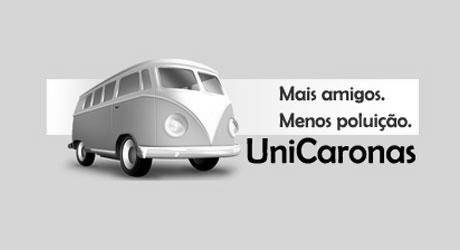
\includegraphics[width=.45\textwidth]{img/barao/unicaronas.jpg}
\end{figure}

O site UniCaronas (\url{unicaronas.com.br}) foi desenvolvido por dois
engenheiros de computação da Unicamp, com o intuito de facilitar o deslocamento
dos alunos entre cidades. Criado em 2007 como Caronas Unicamp e disponível
apenas para alunos da Unicamp, O site chegou a possuir mais de 20 mil usuários e
mediar caronas entre alunos de diversas universidades para várias cidades de
vários estados. Em 2014, o site se uniu ao Tripda (\url{tripda.com.br}),
aumentando imensamente a quantidade de destinos, mas mantendo as funcionalidades
básicas. No entanto, o site serve apenas para colocar os motoristas e caronistas
em contato, não assumindo responsabilidades sobre nenhuma das partes.

Recentemente foi criado o Mural de Caronas\\(\url{muraldecaronas.org}), que
igualmente ao UniCaronas exige um email institucional para realização do
cadastro no site. Entretanto, por enquanto só há opção de carona entre Barão
Geraldo e São Paulo. Além disso, há varios grupos de carona no Facebook, vale a
pena checá-los.

\subsection{Carro}

Para aqueles que tenham seu próprio veículo, é bom saber que a Unicamp tem
poucas vagas próximas aos locais de aulas. E o número de fiscais de trânsito tem
aumentado muito dentro do Campus.

\subsubsection*{Autoescolas}

Se você ainda não tem CNH e pretende obtê-la em Campinas, existem três opções de
autoescola em Barão Geraldo:

\begin{itemize}
    \item \textbf{Auto Escola Avenida} \\Endereço: Av. Albino J. B. De Oliveira,
658 \\Telefone: (19) 3288-0588

    \item \textbf{Auto Escola Advanced} \\Endereço: Av. Santa Isabel, 80
\\Telefone: (19) 3289-9499

    \item \textbf{CFC Brasil} \\Endereço: Av. Santa Isabel, 513
\\Telefone: (19) 3388-0513 / (19) 3289-2614
\end{itemize}

Porém recomendamos fortemente que você tire em sua cidade de origem se isso for
possível; os CFCs de Barão Geraldo são muito caros e muitas vezes você tem que
esperar meses para conseguir marcar aulas.

\subsubsection*{Recorrer de Multas}

Documentos:
\begin{itemize}
    \item Notificação e Fotocopia.
    \item CNH e Fotocopia.
    \item Documento do Carro e Fotocopia.
    \item Formulário:
      \url{bit.ly/1xW5E9z}.
    \item e anexos, se desejar.
\end{itemize}

E levá-los a:
\begin{itemize}
    \item \textbf{EMDEC} \\Horário: De segunda a sexta-feira, das 8h as 17h.
\\Endereço: Rua Dr. Salles Oliveira, 1028 -- Vila Industrial -- CEP 13035-270.
    \item \textbf{Poupatempo (Centro)} \\Horário: Das 8h às 18h, de segunda a
sexta-feira; e aos sábados, das 7h às 13h.  \\Endereço: Av. Francisco Glicério,
935.
    \item \textbf{Poupatempo (Campinas Shopping)} \\Horário: Das 9h às 19h, de
segunda a sexta-feira; e aos sábados, das 8h às 14h.  \\Endereço: Rua Jacy
Teixeira de Camargo, 940.
\end{itemize}

Fonte:
\url{bit.ly/1zntVk4}

\subsection{Ciclovias e ciclofaixas}

Campinas possui cerca de 27 quilômetros de ciclovias e de ciclofaixas. Algumas
dessas vias para bicicletas estão no distrito de Barão Geraldo. Uma delas é a
ciclovia que liga o campus da Unicamp a Av. Albino J. B. de Oliveira. A outra é
a ciclofaixa que liga a Av. Albino J. B. de Oliveira à moradia (Av. Santa
Isabel).

Nos domingos e feriados, das 7 até as 12 horas, as ciclofaixas ficam abertas
para os ciclistas.

\subsection{Ônibus}

Se não tem condução própria, ou carona, pode utilizar o transporte coletivo de
Campinas.

\begin{figure}[h!]  \centering
    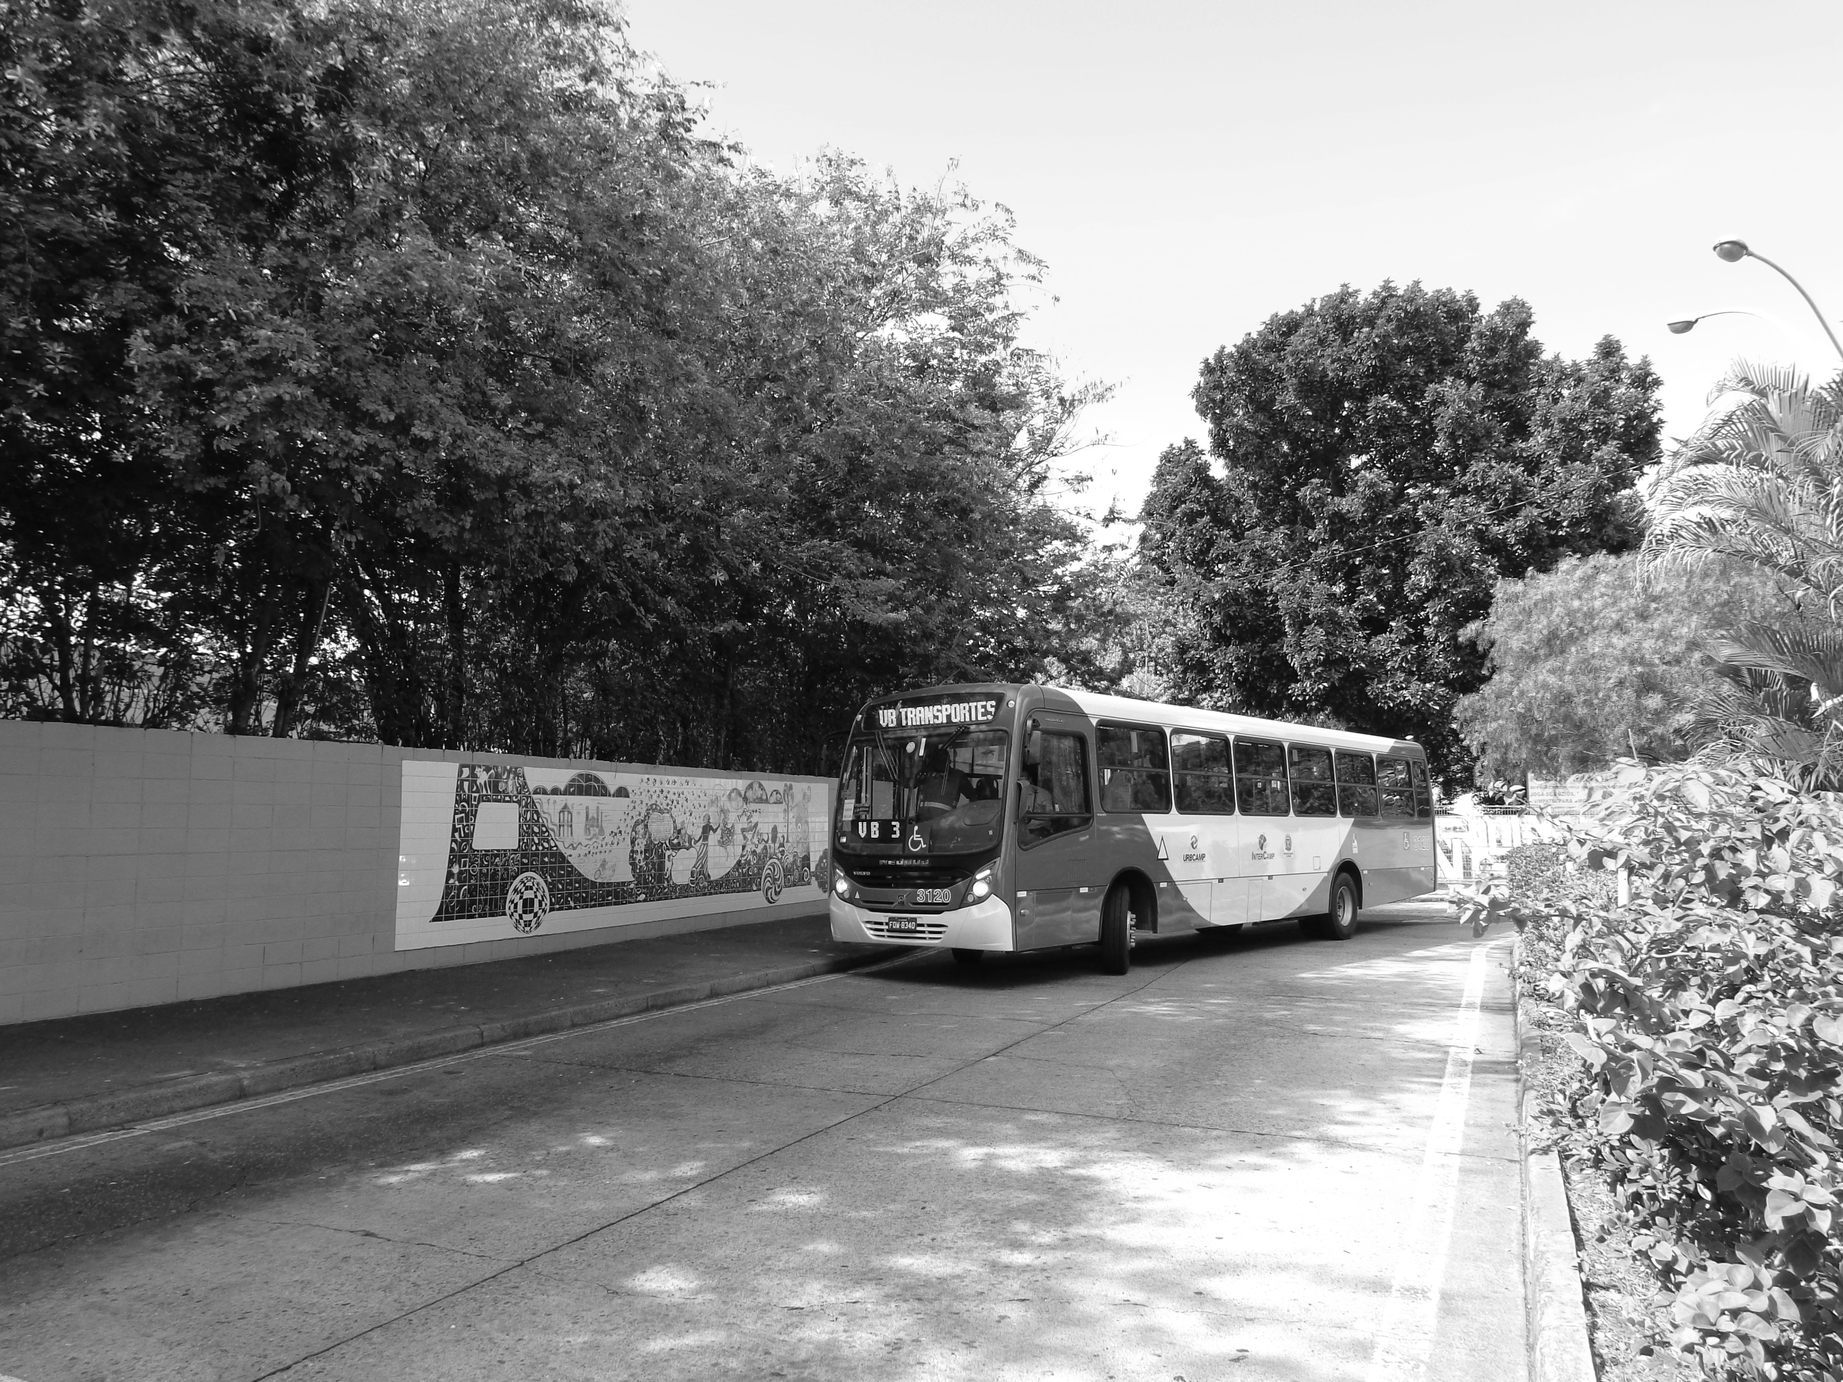
\includegraphics[width=.45\textwidth]{img/barao/onibus.jpg}
\end{figure}

O sistema de transporte público em Campinas é composto apenas por ônibus, e
chama-se InterCamp. O órgão municipal que organiza, gerencia e fiscaliza o
transporte público é a EMDEC (Empresa Municipal de Desenvolvimento de Campinas).
A bilhetagem eletrônica é organizada pela Transurc, a associação das empresas de
ônibus do transporte coletivo urbano de Campinas. Além das empresas, operam no
InterCamp cooperativas de transporte, originadas dos antigos perueiros.

Os ônibus em Campinas são identificados por um número de três dígitos, uma cor
(azul claro, azul escuro, vermelho ou verde), uma figura geométrica (círculo,
quadrado, triângulo ou tetragrama, para que os portadores de daltonismo possam
identificar os ônibus) e um nome.

A tarifa foi reajustada em junho de 2013 e custa R\$3,30. Apesar de existir
passe de estudante, universitários não tinham ao desconto, apenas estudantes de
ensino fundamental e médio. Em dezembro de 2014, o prefeito Jonas Donizete
sancionou lei que concede o desconto da passagem para estudantes universitários
de cursos presenciais.

Todo mês, em dois domingos, os usuários do transporte público de Campinas podem
usar os ônibus pagando metade da tarifa (o que dá R\$ 1,65). É o Passe Lazer. O
benefício vale apenas para os cartões avulsos e para o Bilhete Único Comum.

Existe quatorze linhas de ônibus que ligam o centro, alguns distritos, bairros e
terminais de Campinas ao distrito de Barão Geraldo. Algumas linhas desembarcam
os passageiros no terminal de Barão Geraldo, de onde seguem em outros ônibus
para a universidade. Já outras linhas vão direto para o campus. As trocas de
ônibus dentro do Terminal de Barão Geraldo são gratuitas, o que não ocorre em
outros terminais (no Terminal Mercado, por exemplo).

Em 2008 foi construída a nova e moderna rodoviária de Campinas, o terminal
multimodal Ramos de Azevedo. Além de transporte interestadual e municipal, o
espaço agrega um terminal metropolitano com o intuito de ligar as cidades da
Região Metropilitana de Campinas. Algumas linhas de ônibus internos de Campinas
também passam neste Terminal, como a linha 332.

Para consultar linhas de ônibus, há duas opções:
\begin{itemize}
  \item o sistema da EMDEC, que também possui um roteirizador bastante
interessante (\url{www.emdec.com.br/ABusInf/})
  \item o site Ônibus de Campinas, do Portal InterBuss, criado por entusiastas
de ônibus, dentre eles, um veterano da Computação
(\url{www.portalinterbuss.com.br/campinas/})\ldots
\end{itemize}

Outra ferramenta interessante para quem pretende usar o transporte público em
Campinas é o aplicativo Moovit, disponível para iOS, Android e Windows
Phone. Com ele, é possível visualizar os pontos de ônibus ao seu redor e as
linhas que passam neles. Além disso, também funciona como roteirizador,
indicando as linhas que você pode pegar para chegar a um lugar da cidade.

Para reclamações do transporte público, é necessário utilizar o canal 156 da
Prefeitura de Campinas. Ele pode ser acessado através do telefone 156, através
do site da Prefeitura (\url{www.campinas.sp.gov.br/servico-ao-cidadao/156.php}),
e através do aplicativo 156 Mobile Campinas, disponível para Android. As
reclamações são respondidas pelos órgãos de fiscalização da EMDEC, e todo o
processo pode levar até seis meses. Entretanto, é o único meio que pode resultar
em ações efetivas, como multas e advertências. Além disso, a reclamação entra
nas estatísticas da EMDEC, que são utilizadas para direcionar agentes de
fiscalização e, caso haja algum problema operacional de itinerário ou de
horário, também podem ser feitas alterações para otimização do serviço.

\subsubsection*{Bilhete Único}

O Bilhete Único foi implantado com o objetivo de facilitar o transporte daqueles
que se utilizam de ônibus. No prazo de 2 horas, o usuário pode usar até três
ônibus pagando apenas uma passagem. Além disso, agora o usuário tem dois
créditos negativos para utilizar caso o saldo seja zerado. O cadastro é rápido e
o cartão sai na hora.

O Bilhete Único Comum pode ser feito nos seguintes locais:
\begin{itemize}
  \item sede da Transurc, na Rua Onze de Agosto, 757
  \item nos terminais de ônibus (guichês da Transurc, sempre próximos à entrada)
  \item na Loja do Bilhete Único, na Av. Anchieta, 55
  \item no posto da Transurc do Poupatempo Centro (Av. Francisco Glicério, 935,
térreo)
  \item na Drogaria Sidarta do Balão do Londres (Av. John Boyd Dunlop) \ldots
\end{itemize}

Para a primeira recarga, exige-se o pagamento de uma tarifa (o que atualmente
fica em R\$ 3,30).

Para recarregar o cartão, além dos terminais, também tem diversos
estabelecimentos comerciais credenciados a fazer a recarga do cartão, que podem
ser vistos na página:
\url{bit.ly/13Aav2C}.

\subsubsection*{Como embarcar sem Bilhete Único}

Campinas vem extinguindo a função do cobrador, substituindo-o pela bilhetagem
eletrônica. Várias linhas já rodam sem cobrador, e provavelmente muitos lerão
este texto quando já estiverem completamente extintos do sistema.

A partir de 1º de fevereiro de 2015, o pagamento não poderá mais ser feito em
dinheiro dentro dos ônibus. Com isso, os usuários deverão entrar nos veículos
portando o Bilhete Único (vide sub-seção acima para mais informações) ou um
cartão avulso, chamado Bilhete Viagem.

São dois Bilhetes Viagem: o Bilhete 1 Viagem e o Bilhete 2 Viagens.

O Bilhete 1 Viagem é adquirido pelo valor de R\$ 5,30, e pode ser usado apenas
uma vez, pois não dá direito a integração. Também não pode ser recarregado.  Por
isso, é ideal apenas para quem for utilizar ônibus uma única vez.

O Bilhete 2 Viagens é adquirido pelo valor de R\$ 8,60, pode ser usado por duas
vezes, e depois ainda pode ser recarregado em qualquer posto de recarga do
Bilhete Único. É o cartão ideal para quem pretende utilizar ônibus mais de uma
vez, mas não pretende fazer o Bilhete Único.

Os R\$ 2,00 acima da tarifa vigente pagos na aquisição de ambos os Bilhetes
Viagem se referem ao custo de casco do cartão, que são devolvidos ao usuário se
ele entregar o cartão vazio em um dos postos da Transurc (sede da Transurc,
terminais, Loja do Bilhete Único ou posto da Transurc do Poupatempo Centro).

Ambos os Bilhetes Viagem podem ser adquiridos nos postos da Transurc ou na rede
credenciada
(\url{bit.ly/13Aav2C}).

\newpage
%%%%% Outras necessidades
% Este arquivo .tex será incluído no arquivo .tex principal. Não é preciso
% declarar nenhum cabeçalho

\section{Outras necessidades}
\subsection{Supermercados}

No centro de Barão há três supermercados: o Pague Menos (antigo Super Barão ou
``Super Ladrão'') o Pão de Açúcar e o Dalben. Ambos Pague Menos e Pão de Açúcar
são muito caros, mas o Pague Menos tem boas promoções de segunda e terça-feiras.
Cada um é melhor ou mais barato para alguma coisa. Só indo bastante em cada um é
que você pega o jeito.

\begin{figure}[h!]
    \centering
    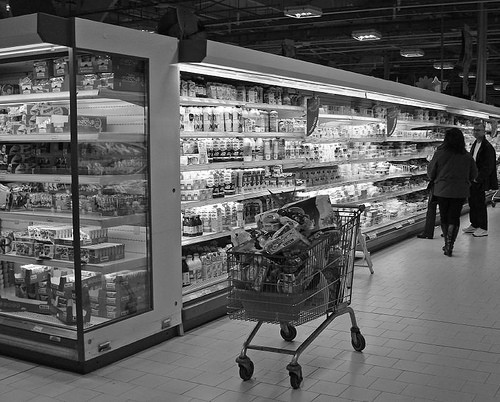
\includegraphics[scale=0.42,keepaspectratio=true]{img/imgs/9-outras_necessidades/supermercado.jpg}
\end{figure}

O Dalben é maior e geralmente tem coisas mais baratas que o Pão de Açúcar. Às
segundas e terças (no Dalben e no Pague Menos) e às terças (no Pão de Açúcar) há
preço promocional de frutas e verduras. O Dalben localiza-se no alto da Avenida
1, na entrada de Barão Geraldo. O Pague Menos funciona de segunda a sábado das
7h às 22h e aos domingos das 8h às 20h, e o Pão de Açúcar funciona de domingo a
quinta-feira das 7h às 23h, às sextas e aos sábados das 7h às 24h. Na moradia,
há outro Pague Menos e o Benatti, e no Real Parque outra loja do Pague Menos.

Há também lojas de conveniência (como as AM/PM em frente à Unicamp na Av. 1, e
no Rio das Pedras e a da Shell no fim da Avenida 2 e em frente ao Terminal, a
mais barata das quatro) que embora mais caras que os supermercados, podem
funcionar em horários alternativos ou serem mais perto de onde você mora.

Em frente ao Terminal Barão há o Recanto Bela Fruta, que não é exatamente um
supermercado, mas é o melhor lugar de Barão para comprar frutas, verduras e
legumes. Vende também algumas coisas de supermercado como pão, leite, iogurte,
Mupy etc. Neste mesmo esquema funciona o varejão Oba, que fica na avenida Santa
Isabel, perto da pizzaria Sapore. Na estrada da Rhodia, depois da Padaria Di
Capri, há a frutaria Rio das Pedras, que tem preços no nível do Pão de Açúcar e
do Pague Menos, mas é mais próximo pra quem vive na Cidade Universitária 2, por
exemplo.

Se você tiver carro, ou conhecer alguém que tenha, junte um pessoal e faça suas
compras no Tenda Atacado ou no Atacadão. Os dois são muito mais baratos que
qualquer supermercado e têm muita variedade. Ah, e nem tudo é atacado, vende
umas coisas a varejo lá também. Para chegar aos dois, saindo de Barão pelo
Tapetão, pegue a D. Pedro sentido Anhanguera. Assim que você entrar na D. Pedro,
você já vai enxergar o Atacadão, à direita. Para ir ao Tenda siga mais um pouco
na D.  Pedro e saia logo depois do CEASA à direita.

Outras opções para quem tem carro são: O Carrefour, localizado na Rodovia D.
Pedro, o Wal-Mart, que fica no Shopping Parque D. Pedro e, andando mais um 
pouquinho na Rodovia D. Pedro, tem o Extra D. Pedro.

\subsection{Utilidades em geral}

\begin{itemize}
    \item  \textbf{Ki-Água}
        \\Telefone: (19) 3289-4659
        \\Endereço: Rua Eduardo Modesto, 240

    \item  \textbf{Circuito das Águas}
        \\Telefone: (19) 3289-4930
        \\Endereço: Rua Júlia Leite de Barros, 182

    \item  \textbf{Água Mineral Serrana}
        \\Telefone: (19) 3289-4602
        \\Endereço: Av. Albino J. B. de Oliveira, 658

    \item  \textbf{Real Gás}
        \\Telefone: (19) 3289-1786
        \\Endereço: Rua Eduardo Pereira de Almeida, 570

    \item  \textbf{Genebra Gás}
        \\Telefone: (19) 3289-3622
        \\Endereço: Av. Santa Isabel

    \item  \textbf{Drogaria Vitória}
        \\Telefone: (19) 3289-9926
        \\Endereço: Av. Ruberley Bueretto da Silva, 1015

    % \item  \textbf{Drogaria Nova Barão}
    %     \\Telefone: (19) 3289-6191

    % \item  \textbf{Rede Farmaxima}
    %     \\Telefone: (19) 3289-2824 / (19) 3289-4054
    %     \\Endereço: Av. Dr. Romeu Tortima, 255

    \item  \textbf{New Laundry Lavanderia}
        \\Telefone: (19) 3289-3922
        \\Endereço: Rua Francisca Resende Merciai, 54

    \item  \textbf{Desentupimento 24 horas}
        \\Telefone: (19) 3242-1249

    \item  \textbf{Carpintaria São Jorge de Barão}
        \\Telefone: (19) 3289-3399
        \\Endereço: Av. Santa Isabel, 1882

    \item  \textbf{CPFL (companhia de luz)}
        \\Telefone: 0800-010-1010

    \item  \textbf{Sanasa (companhia de água)}
        \\Telefone: 0800-772-1195

    \item  \textbf{Luigi Cabelereiro}
        \\Telefone: (19) 3288-0198

    \item  \textbf{João Cabelereiros}
        \\Telefone: (19) 3289-3084
        \\Endereço: Rua Orácio Leonardi, 92

    \item  \textbf{Correios -- Centro de Barão}
        \\Endereço: Av. Santa Isabel, 218 -- Centro de Barão
        \\Telefone: (19) 3288-0244

    \item  \textbf{Correios -- Unicamp}
        \\Endereço: Rua Carlos Gomes, 241 -- Campus da Unicamp (próximo ao ginásio e Instituto de Artes)
        \\Telefone: (19) 3289-7288 / (19) 3521-7642
\end{itemize}

\subsection{Bancos}

\begin{figure}[h!]
    \centering
    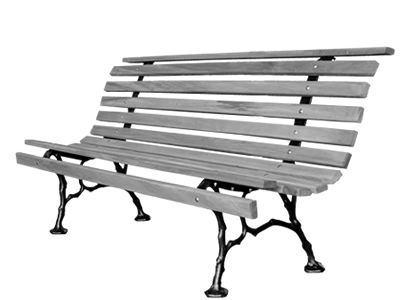
\includegraphics[scale=2.28,keepaspectratio=true]{img/imgs/9-outras_necessidades/raizmadeira.png}
\end{figure}

Bixo, agora que você está na universidade, chegou a hora de tomar vergonha na
cara e abrir uma conta no banco. A menos que você more em Campinas ou muito
perto, essa será a forma principal do papai te mandar dinheiro.

Todos os bancos oferecem algum tipo de conta universitária, que tem tarifas
reduzidas. Os documentos exigidos para abertura de conta costumam ser
identidade, CPF, comprovante de residência (conta de água, luz, telefone, gás --
pode ser do endereço da sua cidade e no nome dos seus pais) e e comprovante de
renda (pode ser no nome dos seus pais).

Além da conta universitária, alguns bancos oferecem uma modalidade de conta
inteiramente sem custo, mas que pode ser operada apenas por meios eletrônicos,
como internet banking, caixa eletrônico, cartão de débito e crédito e telefone.
Enquadram-se nesta categoria as contas eletrônicas do Banco do Brasil e do
Santander e a iConta do Itaú.

Há várias agências bancárias dentro da Unicamp e em Barão Geraldo. Confira onde
se localizam:

\begin{itemize}
    \item  \textbf{Banco do Brasil:} Há três agências: uma localizada perto da
        Reitoria, outra no centro de Barão, perto do Santander, e outra no
        centro de Barão perto do Pague Menos. Há ainda uma agência exclusiva
        para clientes Estilo próxima aos Correios da Unicamp.

    \item  \textbf{Bradesco:} Agência no centro de Barão, do lado do Banco do
        Brasil e em frente do Santander. Próxima ao Terminal Barão.

    \item  \textbf{Caixa Econômica Federal:} Localizada na frente do Pão de
        Açúcar.

    \item  \textbf{Citibank:} Localizado no alto da avenida 2, próximo ao posto
        Shell.

    \item  \textbf{Itaú:} Possui uma agência na Unicamp, próximo à Reitoria e à
        agência do Santander, e outra na avenida Santa Isabel, do lado da
        sorveteria. Existe também o Itaú Personnalité, próximo ao Pão de Açuar e
        ao McDonalds.

    \item  \textbf{Santander:} Há quatro agêncais em Barão: duas localizadas ao
        lado da Reitoria, outra na praça do Ciclo Básico e a outra próxima ao
        Terminal Barão.
\end{itemize}

\subsection{Sebos e livrarias}

Em Barão há três sebos: O Curupira, o Cronópio e o Galpão. Geralmente você não
encontra muita coisa boa de computação neles, mas não custa procurar. O Curupira
fica na rua do Terminal, bem em frente a ele. Não é difícil achar. O Galpão fica
perto do Terminal. Saindo do terminal pela avenida marginal à Albino de
Oliveira, vire a primeira à esquerda e a segunda à direita. Funciona de segunda
à sexta até às 18h. O Cronópio fica na mesma rua do Galpão, só que bem longe,
próximo à padaria Fiori. Seguindo a Santa Isabel, vindo do Centro de Barão, vire
à esquerda na esquina que tem uma pizzaria (antes da Fiori). Vire na primeira à
esquerda e você está no Cronópio (Lá também é um restaurante barato e gostoso).

Na Unicamp há a livraria Toledo, que fica na Faculdade de Educação (Pedago), tem
pouca coisa de Computação lá, mas sempre tem alguma coisa de Matemática. Também
há a livraria da Unicamp (no IEL), tem preços bons mas não tem quase nada de
Exatas. Já a Livraria da Química tem livros de exatas, e geralmente eles
conseguem importar a um preço bom. Outras livrarias são a Fnac (no Shopping D.
Pedro), a Saraiva e a Cultura (no Shopping Iguatemi) e a Siciliano (no Shopping
Galeria).

Mais uma dica: Antes de comprar um livro, veja se você vai usar muito ele, se
não tem bastante na biblioteca, se algum veterano legal não pode te emprestar ou
te vender, ou se não rola tirar xerox. Você compra livro só se você precisar
e/ou quiser muito. Caso vá comprar, atente para livrarias virtuais, que podem
ter preços muito menores (pesquise sempre no Buscapé (\url{buscape.com.br})) e
emitem boletos para você pagar no banco.  Em alguns casos, a livraria da Editora
(localizada no piso térreo da BC) pode trazê-lo por um preço menor ainda --
consulte sempre!

Uma última dica: Não compre o livro de G.A. (MA141). Estude pelo Stewart II
(livro de Cálculo II), pelo Steinbruch ou pelo livro do Paulo Boulos. Os três
são muito melhores que ele. Se você quiser os exercícios para estudar para os
testes pegue na internet ou tire xerox. Use os outros livros para estudar.

\begin{figure}[h!]
    \centering
    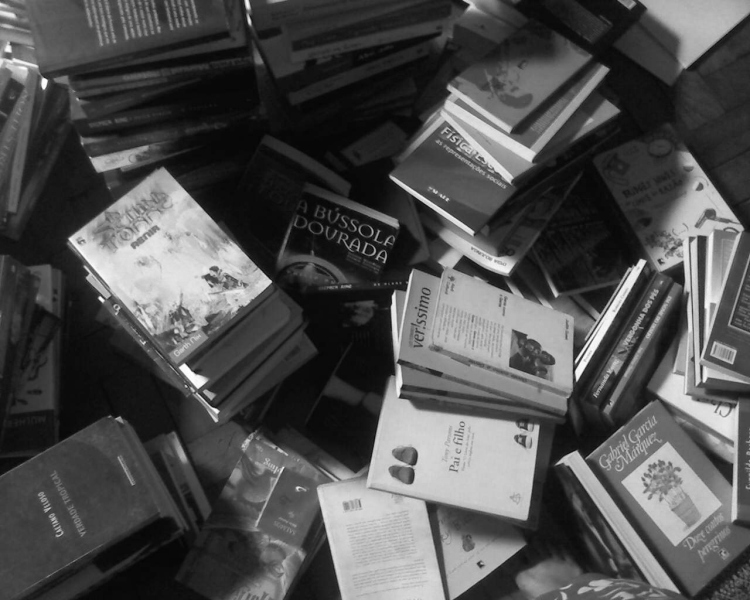
\includegraphics[scale=0.29, keepaspectratio=true]{./img/imgs/9-outras_necessidades/-068.jpg}
\end{figure}


\begin{itemize}
    \item   \textbf{Sebo Galpão}
        \\Endereço: Rua Francisco Barros Filho, 16
        \\Telefone: (19) 3289-2044

    \item   \textbf{Sebo Valise de Cronópio}
        \\Endereço: Rua Francisco de Barros Filho, 426
        \\Telefone: (19) 3289-0028
\end{itemize}

\subsection{Bicicletarias}

\begin{itemize}
    \item   \textbf{Rei do Pedal}
        \\Endereço: Av. Santa Isabel, 74
        \\Telefone: (19) 3289-9258

    \item   \textbf{Via Bike}
        \\Endereço: Av. Albino J. B. de Oliveira, 1074
        \\Telefone: (19) 3289-9888
\end{itemize}

\subsection{Escolas de idiomas}

\begin{itemize}
    \item   \textbf{CCAA}
        \\Endereço: Rua Prof. Luciano Venere Decourt, 290
        \\Telefone: (19) 3249-0202
        \\E-mail: \email{barao@ccaa.com.br}
        \\Site: \url{ccaa.com.br/barao}

    \item   \textbf{CCBEUC -- Centro Cultural Brasil Estados Unidos -- Campinas}
        \\Endereço: Av. Dr. Romeu Tortima, 531
        \\Telefone: (19) 3249-0275
        \\E-mail: \email{admbg@ccbeuc.com.br}
        \\Site: \url{ccbeuc.com.br}

    \item   \textbf{CNA}
        \\Endereço: Av. Dr. Romeu Tortima, 553
        \\Telefone: (19) 3289-4700
        \\Fax: (19) 3289-4700
        \\E-mail: \email{baraogeraldo@cna.com.br}
        \\Site: \url{cna.com.br/baraogeraldo}

    \item   \textbf{HAVAD}
        \\Endereço: Av. Dr. Romeu Tortima, 522
        \\Telefone: (19) 3288-0012
        \\Fax: (19) 3249-0488
        \\E-mail: \email{havad@havad.com.br}
        \\Site: \url{havad.com.br}

    \item   \textbf{In Touch}
        \\Endereço: Rua Antônio Augusto de Almeida, 517 -- Cidade Universitária
        \\Telefone: (19) 3289-3481
        \\E-mail: \email{secretaria@intouch.art.br}
        \\Site: \url{www.intouch.art.br}

    \item   \textbf{INOVA -- Escola de Inglês}
        \\Endereço: Av. Dr. Romeu Tortima, 391
        \\Telefone: (19) 3288-0071
        \\E-mail: \email{fale@inovalinguas.com.br}
        \\Site: \url{inovalinguas.com.br}

    \item   \textbf{Skill Idiomas}
        \\Endereço: Rua Agostinho Páttaro, 47 (esquina com a do praça do coco)
        \\Telefone: (19) 3289-6240

    \item   \textbf{Wizard}
        \\Endereço: Rua João Batista Antonioli, 90
        \\Telefone: (19) 3289-6199
        \\Site: \url{wizard.com.br}

    \item   \textbf{Yazigi}
        \\Endereço: Av. Dr. Romeu Tortima, 500
        \\Telefone: (19) 3249-2375
        \\Site: \url{yazigi.com.br}
\end{itemize}

\subsection{Igrejas}

\begin{itemize}
    \item   \textbf{IBCU -- Igreja Batista da Cidade Universitária}
        \\Endereço: Rua Tenente Alberto Mendes Jr., 5
        \\Telefone: (19) 3289-4501
        \\E-mail: \email{jovens@ibcu.org.br}
        \\Site: \url{ibcu.org.br}

    \item   \textbf{IBBG -- Igreja Batista de Barão Geraldo}
        \\Endereço: Rua Luiz Vicentim, 284
        \\Telefone: (19) 3289-1793

    \item   \textbf{IPBG -- Igreja Presbiteriana de Barão Geraldo}
        \\Endereço: Rua Francisco Andreo Aledo, 141 (próximo à praça do coco e moradia)
        \\Telefone: (19) 3289-3239

    % \item   \textbf{Igreja do Nazareno Betânia}
    %     \\Endereço: Rua Manoel Antunes Novo, 98
    %     \\Telefone: (19) 3289-7379

    % \item   \textbf{Assembleia de Deus -- Ministério de Belém}
    %     \\Endereço: Rua Júlia Leite de Barros, 54 (próximo à moradia da Unicamp)
    %     \\Telefone: (19) 3249-0035
    %     \\Site: \url{adbarao.com.br}

    \item   \textbf{Paróquia Santa Isabel}
        \\Endereço: Rua Benedito Alves Aranha, 226
        \\Telefone: (19) 3289-1101 / (19) 3289-2323
        \\Site: \url{www.paroquiasantaisabel.org.br}

    \item   \textbf{Comunidade do Estudante Universitário}
        \\Endereço: Rua Dr. Ruberlei Boaretto da Silva, 785
        \\E-mail: \email{ceu.campinas@gmail.com}
\end{itemize}

\subsection{Postos de combustível}

\begin{itemize}
    \item   \textbf{Auto Posto Campineira}
        \\Endereço: Av. Albino J. B. de Oliveira, 1480
        \\Telefone: (19) 3289-5991

    \item   \textbf{Auto Posto Barbieri de Barão Geraldo}
        \\Endereço: Av. Albino J. B. de Oliveira, 1001 (próximo ao terminal)
        \\Telefone: (19) 3289-1917

    \item   \textbf{Centro Automotivo Cidade Universitária LTDA}
        \\Endereço: Av. Dr. Romeu Tortima, 1541
        \\Telefone: (19) 3289-8457 / (19) 3289-9934

    \item   \textbf{Transo Combustíveis LTDA}
        \\Endereço: Av. Santa Isabel, 1030 (próximo à moradia)
        \\Telefone: (19) 3289-1012

    \item   \textbf{Esso Auto Posto Futuro}
        \\Endereço: Av. Albino J. B. de Oliveira, 360 (logo na entrada do distrito de Barão)
        \\Telefone: (19) 3289-4332

    \item   \textbf{Posto Vô João}
        \\Endereço: Av. Albino J. B. de Oliveira, 2151
        \\Telefone: (19) 3289-3388 / (19) 3289-6594
        \\E-mail: \email{vojoao@vojoao.com.br}
        \\Site: \url{vojoao.com}
\end{itemize}

OBS: Dentro do campus há um posto de combustível (próximo à descida da FEAGRI),
mas atende apenas veículos oficiais.


\chapter{Estudando na Unicamp}
%%%%% SIGLAS malucas
% Este arquivo .tex será incluído no arquivo .tex principal. Não é preciso
% declarar nenhum cabeçalho

\section{SIGLAS malucas}

Nesta sessão serão dadas algumas explicações sobre algumas siglas, códigos e
outros termos muito usados dentro da Unicamp. Aí vão eles:

\subsubsection{CCG (Comissão Central de Graduação):} Órgão colegiado da Unicamp,
é encarregada da orientação, supervisão e revisão periódica do ensino na
Universidade. Cabe recurso à CCG de quaisquer decisões das Unidades afetando o
ensino.

\subsubsection{CCPG (Comissão Central de Pós-Graduação):} Órgão colegiado da
Unicamp, é encarregada da orientação, supervisão e revisão periódica da
pós-graduação na Universidade. Cabe recurso à CCPG de quaisquer decisões das
Unidades afetando o ensino.

\subsubsection{Consu (Conselho Universitário):} O Consu é o órgão máximo da
Universidade, acima do reitor, embora ele faça parte e influencie fortemente
suas decisões.  Existe representação discente no Consu, eleita juntamente com a
Coordenadoria do DCE.

\subsubsection{Congregação:} É o órgão colegiado máximo do instituto ou
faculdade.  Cabe recurso à Congregação da Unidade de Ensino de quaisquer
decisões dos Departamentos e das Coordenações de Curso. Os representantes
discentes na Congregação do IC atualmente são: \textbf{Pedro Rodrigues Grijó}
(\email{pedrgrijo@gmail.com}) e \textbf{Gabriel Militão}
(\email{gabrielopes13@gmail.com}), esse último também na FEEC.

\subsubsection{Departamento:} É administrado por um professor-chefe e um
Conselho Departamental, é a menor unidade administrativa, didática e científica
da Universidade, sendo responsável pelo desenvolvimento dos programas de ensino,
pesquisa e extensão dos serviços à comunidade. Todo instituto e faculdade da
universidade possui o seu conjunto de departamentos, conhecidos através de
siglas.

\subsubsection{CI (Conselho Interdepartamental):} Este é um ``braço'' da
Congregação, responsável por tratar de assuntos menores, como despesas e
atribuições de sala. Fazem parte deste órgão, além de um representante discente,
o diretor do instituto, os coordenadores e os chefes de departamentos. No IC, o
representante discente atual é \textbf{Alex Wei} (\email{alex290396@gmail.com}).

\subsubsection{CDI (Comissão Diretora de Informática):} Outro braço da
congregação, responsável por tratar de assuntos relacionados aos ambientes
computacionais, deliberando sobre a atualização de infraestrutura, a organização
da rede, endereços de internet e similares.

\subsubsection{CG (Coordenadoria/Comissão de Graduação):} É o órgão da unidade
responsável pelos seus cursos de graduação. Sempre que houver algum problema ou
deficiência no curso, é este órgão que vocês devem procurar.  Cada curso tem um
coordenador (que faz parte da CG), sendo que, atualmente, o professor Eduardo
Xavier é o coordenador da Ciência e os professores Hélio Pedrini (IC) e Rafael
Mendes (FEEC) são os coordenadores da Engenharia. A CG também conta com
representantes discentes. Eles devem ser sua primeira forma de comunicação com a
CG.  Atualmente, os representantes discentes na CG do IC são: \textbf{Pedro
Emilio Machado de Brito} (\email{pedroembrito@gmail.com}), da Engenharia, e
\textbf{Yuri Soares} (\email{yuricorreapinto@gmail.com}), da Ciência.

\subsubsection{CPG (Coordenadoria/Comissão de Pós-Graduação):} Este é o órgão
responsável pela pós-graduação no Instituto, coordenando as disciplinas
oferecidas e as matrículas na pós. O coordenador atual é o professor Paulo Lício
de Geus.

\subsubsection{DCE (Diretório Central de Estudantes):} É a entidade de
representação dos estudantes de graduação da Unicamp, competindo-lhe ainda
designar representantes estudantis para os órgãos colegiados da Universidade.

\subsubsection{DAC (Diretoria Acadêmica):} É o órgão executivo e informativo,
incumbido do registro e controle das atividades discentes da Unicamp. Cuida das
matrículas, alteração de matrícula, emissão de documentos e relatórios, como o
histórico escolar, realiza reserva de salas, entre outras atividades.

\begin{figure*}[hb!]  \centering
  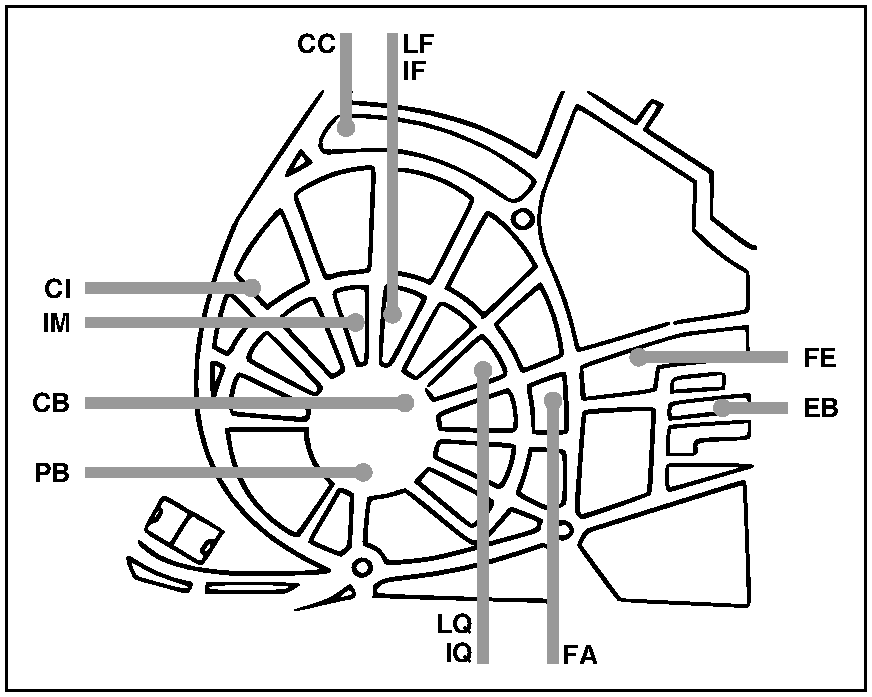
\includegraphics[width=\textwidth]{img/unicamp/mapa_siglas.pdf}
  \caption{Mapa com as siglas da sala de aula}
  \label{fig:mapa_siglas}
\end{figure*}

\subsubsection{SAE (Serviço de Apoio ao Estudante):} É encarregado da execução
de programas de assistência desenvolvidas pela Universidade, por iniciativa
própria ou mediante convênios firmados com entidades especializadas.

\subsubsection{Crédito:} Unidade elementar de horas-aula de qualquer curso da
Unicamp. Um crédito equivale a uma hora-aula semanal, ou a 15 horas-aula
semestrais.

\subsubsection{Período letivo:} É um nome complicado para se referir ao
semestre.

\subsubsection{Currículo pleno:} É o conjunto de disciplinas do curso que o
aluno tem que cursar.

\subsubsection{CR (Coeficiente de Rendimento):} Valor entre 0 e 1 que é a média
ponderada das notas obtidas em todas as disciplinas até o momento.  É calculada
usando como pesos o número de créditos de cada disciplina.

\subsubsection{CP (Coeficiente de Progressão):} É a porcentagem do curso que
você já cumpriu. Por exemplo, se você tem CP = 0,6123 significa que você cumpriu
61,23\% do curso. Você se forma quando o seu CP for 1 (100\% do curso
completo). É importante saber o CP quando for fazer algum estágio, ou um TCC
(Trabalho de Conclusão de Curso), ou quando for cursar disciplinas que tenham
como pré-requisito AA4xy.

\subsubsection{CPF (Coeficiente de Progressão Futuro):} Além do CP, também tem o
CPF, que além do nome de um documento é o CP que você terá no fim do semestre
caso passe em todas as disciplinas.

\subsubsection{CPE (Coeficiente de Progressão Exigido):} Além do CP e do CPF há
o CPE. O CPE foi instituído a partir de 2005 e é usado para fins de
cancelamento, ou não, de matrícula. Para que o aluno possa continuar a fazer o
curso, ele precisa ter um CP maior ou igual ao CPE daquele semestre. Tanto o CP,
como o CPE e o CPF existem somente nos cursos de graduação.

\subsubsection{Pré-requisito:} Matéria(s) que precisa(m) ter sido cursada(s)
para que se possa fazer outra(s) matéria(s). Existem dois tipos de
pré-requisitos: Os pré-requsitos totais, mais comuns, do qual é exigido tanto a
aprovação por nota como por frequência e os pré-requisitos parciais, mais raros,
do qual o aluno não precisa ter sido aprovado por nota, mas tem que ter tido
aprovação por frequência e nota final maior ou igual a 3,0. Os pré-requisitos
parciais são identificados com um asterisco na frente do código da disciplina
(não confundir com um apontador).

\subsubsection{AA4xy:} Um tipo de pré-requisito. Não se trata de nenhuma
disciplina. Para fazer disciplinas com esse pré-requisito, o aluno tem que tem
um CP maior ou igual a 0,xy.

\subsubsection{AA200:} Outro tipo de pré-requisito existente, mais presente em
disciplinas eletivas. Também não se trata de nenhuma disciplina. É apenas uma
autorização da coordenadoria do curso. Se sobrar vagas para a disciplina e a
coordenadoria do curso for com a sua cara você faz a disciplina.

\subsubsection{PB (Prédio Básico)} Também conhecido como Ciclo Básico II, é um
prédio com várias salas de aula, que fica em frente ao Bandejão, e serve várias
unidades que não possuem espaço físico suficiente para comportar seus alunos. No
segundo andar ficam as salas de aula (PB01 a PB12) e no terceiro andar ficam os
auditórios (PB13 a PB18).

\subsubsection{CB (Ciclo Básico I):} Tem finalidade idêntica ao PB, só que é
muito melhor equipado, tem uma acústica muito melhor e tem um ar condicionado
capaz de matar esquimó de frio. Fica na mesma praça que o PB, só que no outro
extremo. À esquerda da entrada ficam as salas ímpares e à direita ficam as salas
pares. No primeiro andar ficam os auditórios (CB01 a CB06) que possuem 140 e 160
lugares e no segundo andar ficam as salas de aula (CB07 a CB18) que possuem 60 e
80 lugares.  O CB e o PB são os lugares onde você vai ter a maioria das suas
aulas (especialmente nos dois primeiros anos de curso).

\subsection{Siglas de salas de aula}

A Tabela~\ref{tab:institutos} contém algumas siglas de salas de aula que
aparecem nos cadernos de horários, disponibilizados pelas coordenadorias dos
cursos e pela DAC. E a Figura~\ref{fig:mapa_siglas} aponta a localização das
salas de aula pelas siglas.

\begin{table*}[ht!]
    \centering
    \begin{tabular}{|c|p{.4\textwidth}|p{.45\textwidth}|}\hline
        \multicolumn{3}{|c|}{ \textbf{Siglas e locais das Salas de Aula no horário}}\\ \hline

        \textbf{Sigla}  &  \textbf{Local}  &  \textbf{Referência}\\ \hline

        CB  &  Ciclo Básico I  &  Praça Central, atrás do Santander, em frente à Cantina da Física.\\ \hline

        CC  &  Instituto de Computação (IC)  &  Ao lado do Departamento de Artes Cênicas (IC-1); ao lado do IE (IC-2) e atrás do IE (IC-3).\\ \hline

        CI  &  Centro de Estudo de Línguas (CEL)  &  Atrás do IFCH.\\ \hline

        CL  &  Instituto de Estudos da Linguagem (IEL)  &  Em frente a praça central e ao lado do IFCH.\\ \hline

        EB  &  Engenharia Básica  &  Atrás da Praça da Paz e próximo à FEEC.\\ \hline

        EM  &  Faculdade de Engenharia Mecânica (FEM)  &  Atrás do IQ.\\ \hline

        FA  &  Faculdade de Engenharia de Alimentos (FEA)  &  Em frente ao IQ e à Praça da Paz.\\ \hline

        FE  &  Faculdade de Engenharia Elétrica e de Computação (FEEC)  &  Em frente à Praça da Paz.\\ \hline

        IB  &  Instituto de Biologia (IB)  &  Entre o IQ e o Serviço Social do SAE.\\ \hline

        IE  &  Instituto de Economia (IE)  &  Atrás do IMECC.\\ \hline

        IF  &  Instituto de Física (IFGW)  &  Em frente ao Ciclo Básico, e a Química.\\ \hline

        IH  &  Instituto de Filosofia e Ciências Humanas (IFCH)  &  Entre o IMECC e o IEL.\\ \hline

        IM  &  Instituto de Matemática, Estatística e Computação Científica (IMECC)  &  Em frente a Praça Central.\\ \hline

        IQ  &  Instituto de Química (IQ)  &  Entre o IB e o IFGW.\\ \hline

        LE  &  Laboratórios de informática da FEEC  &  Em frente a Praça da Paz e ao lado das salas de aula da FEEC.\\ \hline

        LF  &  Laboratório de Física  &  Em frente à cantina do IMECC.\\ \hline

        LQ  &  Laboratório de Química  &  Em frente à biblioteca do IQ.\\ \hline

        PB  &  Ciclo Básico II, Prédio Básico  &  Praça Central, em frente ao Bandejão.\\ \hline
    \end{tabular}
    \caption{Siglas das salas de aula}
    \label{tab:institutos}
\end{table*}

\newpage
%%%%% Disciplinas
% Este arquivo .tex será incluído no arquivo .tex principal. Não é preciso
% declarar nenhum cabeçalho

\section{Disciplinas}

\subsection{Matrícula}

A Unicamp é muito diferente da sua escolinha onde a tia Gertrudes entregava o
seu horário impresso coloridinho para você colar na capa do seu fichário.  À
exceção do primeiro semestre letivo, no qual você já entra matriculado em todas
as matérias obrigatórias, na Unicamp você vai ter que se virar.  O GDE
(\url{gde.ir}) é uma ferramenta criada por um aluno da Engenharia e adotada pela
DAC que facilita muito o planejamento do seu horário, além de servir como uma
rede social interna.

Peça sempre a ajuda dos seus veteranos quando for montar seu horário. Informe-se
sobre todos os professores que oferecem as matérias, se eles são coxas ou
carrascos, bons ou ruins, se demoram para entregar as notas{\dots} Você vai
poupar muita dor de cabeça. O melhor lugar para essas discussões é o grupo de
e-mail da sua turma.  Pode ter certeza que ela terá um assim que você entrar na
Unicamp.

\subsection{Cancelamento, Trancamento e Desistência}

Embora praticamente todos os alunos da Unicamp usem esses três termos
indiscriminadamente, como se fossem sinônimos, para a DAC, esses três termos têm
significados bastante distintos. Aí vai o que cada termo significa:

\begin{itemize}
    \item Desistência de matrícula em disciplinas
        (\url{www.dac.unicamp.br/portal/grad/regimento/capitulo_iii/secao_v}):
        Processo que é chamado pelos alunos de ``trancamento''.  O aluno não
        mais cursa essa disciplina no semestre, tendo de cursá-la em algum
        semestre posterior. Só é possível desistir uma vez da disciplina e
        pode-se pedir desistência até que se tenha passado metade do semestre.
    \item Cancelamento de matrícula
        (\url{www.dac.unicamp.br/portal/grad/regimento/capitulo_iii/secao_vii}):
        Processo em que o aluno se desliga da Unicamp, por motivo de jubilação,
        por ter faltado às duas primeiras semanas do ano de ingresso, por ter
        sido reprovado em todas as disciplinas do primeiro ou do segundo
        semestre de ingresso, por ter sido expulso, por ter sido aprovado em
        outra universidade pública (não é permitido fazer mais do que um curso
        de universidade pública simultaneamente), ou por vontade própria do
        aluno.
    \item Trancamento de matrícula
        (\url{www.dac.unicamp.brportal/grad/regimento/capitulo_iii/secao_vi}):
        Processo em que o aluno não cursa qualquer disciplina da Unicamp durante
        o semestre. O aluno tem direito a fazer até dois trancamentos de
        matrícula, em semestres seguidos ou não e o aluno não pode trancar
        nenhum dos dois semestres do ano de ingresso. Desistência de todas as
        disciplinas configura-se como trancamento. O trancamento é pedido na
        DAC, e pode ser pedido até que se tenha transcorrido 2/3 do semestre
        (geralmente de dezembro até fim de maio para trancamento de primeiro
        semestre; e de julho até fim de outubro para trancamento de segundo
        semestre). Para cada trancamento, o prazo máximo de integralização é
        postergado.
\end{itemize}

\subsection{Eletivas e Teste de Proficiência}

A Unicamp oferece a seus alunos a oportunidade de personalizar seu currículo de
acordo com seu interesse por meio das \textbf{disciplinas eletivas}. Ao
contrário das disciplinas obrigatórias, com as eletivas você pode escolher a
matéria que vai cursar. Alguns créditos podem ser cumpridos com qualquer
disciplina oferecida pela Universidade, outros estão restritos a um determinado
conjunto. Para mais detalhes, consulte seu catálogo em
\url{www.ic.unicamp.br/graduacao/catalogos-de-graduacao}.

Mas não se esqueça de que com um grande poder vem uma grande responsabilidade!
A Unicamp lhe dá liberdade para escolher o melhor jeito de se preparar para seu
futuro, e espera que você saiba o que fazer com essa liberdade. Você pode
socializar com outros cursos, aprender uma língua estrangeira, assistir a
seminários ou obter um certificado de estudos na FEEC ou no IC.

\textbf{Teste de proficiência} é uma prova que permite dispensa de cursar uma
disciplina (desde que você obtenha a nota mínima, é claro). Se você acha que
sabe o suficiente sobre eletromagnetismo, por exemplo, pode tentar a
proficiência de Física Geral III.  Nem todas as disciplinas oferecem o teste, e
você só pode fazê-lo uma vez por disciplina -- e se você já se matriculou na
disciplina e não passou, não pode fazer.  Além disso, fazer o teste de
proficiência também é obrigatório para se matricular nas disciplinas de língua
inglesa e japonesa, independentemente de conhecimento prévio na língua.

Fique ligado no calendário da DAC para não perder as datas de inscrição nos
testes de proficiência! As datas dos testes de línguas são sempre no começo do
ano, diferentes das demais, que são no fim de cada semestre.

Disciplinas eletivas e teste de proficiência estão relacionados porque muitas
pessoas, especialmente nos cursos de computação, fazem proficiência em
disciplinas de línguas, eliminando créditos de eletivas, em alguns casos para
evitar o jubilamento, outros para não ter que passar mais um semestre na
faculdade. Apesar de registrar a familiaridade do aluno com uma outra língua em
sua integralização, essa prática não enriquece a graduação de nenhum estudante
que faça tal escolha. Além disso, muitos bixos arrependem-se de terem feito a
prova e perdido preferência na hora de pegar uma disciplina interessante,
podendo até mesmo não conseguir se matricular. Isso acontece porque, depois que
seus créditos de eletivas se esgotam, você começa a puxar matérias
não-obrigatórias como \textbf{extracurriculares} e tem prioridade menor na
atribuição de vagas.

Converse com seus amigos e veteranos para descobrir o melhor jeito de usufruir
dessa liberdade que poucas universidades oferecem! Dificilmente você não
encontrará algo com o qual se identifica ou que não ensine lições interessantes.

Para mais informações sobre teste de proficiência, acesse:
\url{www.dac.unicamp.br/portal/grad/avaliacao_e_frequencia/teste_de_proficiencia}.

\subsection{Avaliações de professores}

Achou que o professor ensinou muito mal? Ele falou da vida, do universo e tudo
mais -- menos sobre a disciplina? Foi incoerente? Ou, pelo contrário, achou o
professor o máximo e a sala do CB a oitava maravilha do mundo? Não adianta
xingar nem elogiar no Twitter!

Nas últimas aulas de cada semestre, todos os professores devem disponibilizar um
formulário de avaliação. Esse é o momento para que você possa separar os acertos
dos erros, portanto preencha com seriedade. Os dados serão analisados pelas
Comissões de Graduação de cada unidade e os comentários escritos serão
repassados para o professor.

Além dos formulários, a PRG (Pró-reitoria de Graduação) realiza o Programa de
Avaliação da Graduação no fim de cada semestre. Trata-se de uma pesquisa on-line
semelhante aos formulários de cada unidade, porém unificada para toda a Unicamp
e mais abrangente em suas perguntas.

O GDE (\url{gde.ir}) também tem um sistema de avaliação de professores, cuja
nota costuma ser usada pelos alunos como um dos critérios no momento de decidir
com que professor puxar uma matéria.

Durante o semestre, ocorre a Reunião de Avaliação de Curso. A data e o horário
serão divulgados pelas unidades e pelo CACo. Essa é uma oportunidade de passar
para as coordenadorias do curso não só suas impressões sobre professores e
disciplinas, mas sobre qualquer assunto relacionado ao curso. Antes da Reunião,
o CACo também promove um PipoCACo de Avaliação de Curso, motivando uma
pré-discussão.

Tenha sempre em mente que a nossa percepção sobre o oferecimento de uma
disciplina não é óbvia para os professores. Preencha todas as avaliações com
sinceridade e use sempre os espaços dedicados a comentários. Além disso, cultive
o hábito de realizar uma avaliação informal do professor no fim de cada semestre
-- mandando um e-mail, por exemplo. O valor deste tipo de avaliação é muito
grande.

\newpage
%%%%% Lugares para estudar
% Este arquivo .tex será incluído no arquivo .tex principal. Não é preciso
% declarar nenhum cabeçalho

\section{Lugares para estudar}

Há vários lugares para estudar na Unicamp. Você pode escolher o que você achar
melhor:

\begin{itemize}
    \item  \textbf{Biblioteca Central (BC):} A BC tem três andares. O primeiro é
        onde tem os livros gerais e onde a galera estuda. Geralmente é
        barulhento em épocas de provas, mas é bom porque sempre tem lugar para
        estudar e fecha às 22h.  Se você não se importa com barulho, ou até acha
        que você faz bastante, esse é o lugar da BC para você estudar. O segundo
        andar é onde está a BAE, a Biblioteca da Área de Engenharia. Um pouco
        mais silenciosa que a BC nas mesas externas, esse andar tem salas para
        estudo em grupo, bastante silenciosas, mas que sempre estão ocupadas em
        época de provas, e mesas individuais escondidas entre os periódicos. O
        terceiro andar é para silence freaks. Morbidamente silencioso, desértico
        (muita gente desconhece a existência desse andar), esse é o lugar mais
        silencioso da BC para estudar. Tem umas salinhas de estudo individual e
        duas mesas para estudo em grupo. O problema é que fecha às 17h, mas o
        pôr-do-sol de lá de cima também é ma-ra-vi-lho-so.

        \begin{figure}[h!]
            \centering
            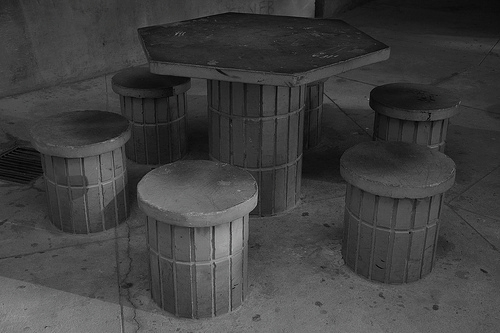
\includegraphics[width=.45\textwidth]{img/unicamp/mesinhas.jpg}
        \end{figure}

    \item  \textbf{Arcádia (ou mesinhas do IEL):} A Arcádia é algumas mesas ao
        ar livre no IEL (Instituto de Estudos da Linguagem). Em horários de aula
        é silencioso, é um ambiente muito agradável e por ser ao ar livre, não
        fecha.  Tem dois problemas: O grande fluxo de pessoas no local pode
        facilmente distraí-lo, principalmente se você as conhecer, e à noite
        enche de insetos (além da iluminação não ser das melhores). Às vezes,
        venta bastante e é ruim para estudar com folhas avulsas. Mas ainda assim
        é um ótimo local para estudar.

    \item  \textbf{Biblioteca do IFGW:} A biblioteca do IFGW (Instituto de
        Física Gleb Wataghin) é ótima para dias de calor, por ser super gelada
        (ar-condicionado mega-super-power!). Tem vantagem sobre as outras
        bibliotecas pelo fato das salas de estudo serem fora da biblioteca e por
        isso você não precisa deixar o seu material para entrar na sala de
        estudos. Recentemente reformada, agora conta com 6 salas para estudo em
        grupo e quantidade razoável de baias individuais, algumas com tomadas
        onde você pode plugar seu notebook. Recentemente as salas em grupo
        passaram a ficar trancadas, é preciso deixar o RA pra pegar a chave, e
        algumas são reservadas para alunos da Física.

    \item  \textbf{BIMECC:} A biblioteca do IMECC tem poucos lugares, poucas
        mesas para estudo individual, os locais de estudo ficam dentro da
        biblioteca (você precisa guardar sua bolsa para entrar), não é muito
        gelada e o ambiente não é agradável, mas nela e na BAE é que você
        encontrará a maioria dos livros relacionados a computação.

    \item  \textbf{Outras bibliotecas:} Aventure-se por outras bibliotecas, como
        a da Economia, a da Pedago e a da Biologia e as conheça. Para aqueles
        que gostam (ou são obrigados) a estudar aos fins de semana a BC e as
        bibliotecas da Educação, da Economia, da Química, da Medicina, do IEL e
        da Geociências abrem aos sábados. Para saber os horários de
        funcionamento das bibliotecas, entre no site do SBU
        (\url{www.sbu.unicamp.br/portal/index.php?Itemid=139}).

    \item  \textbf{Bitolódromos:} Existem dois bitolódromos na Unicamp: O do IC
        e o da FEEC (coincidência interessante, né?). O do IC-3 é uma mesa
        grande com algumas cadeiras no corredor dos laboratórios. O da FEEC fica
        no fundo do prédio principal (qualquer veterano sabe onde é o
        bitolódromo, não tenha vergonha de perguntar). O da FEEC é maior, você
        se distrai menos porque não estão todos os seus colegas (mas várias
        outras pessoas estão) entrando e saindo de lá (embora os pica-fios sejam
        bastante barulhentos), e sempre você encontra gente que possa te ajudar.
        O do IC serve para quando você já estiver lá e com preguiça de ir à
        Elétrica, porque o da FEEC é muito melhor. Exceto talvez se você precisa
        da rede sem fio, já que a da FEEC tem cobertura falha.

    \item  \textbf{Sala 316:} Outro alento para as madrugadas de estudo é a sala
        316 do IC-3, que fica aberta sempre, ou então, aberta facilmente com a
        chave em posse do guardinha. É uma sala com carteiras legais, lousa e ar
        condicionado, aliás, é muito boa para estudo em grupo (NABVS IMINENTVS)
        por causa da lousa.

        \begin{figure}[h!]
            \centering
            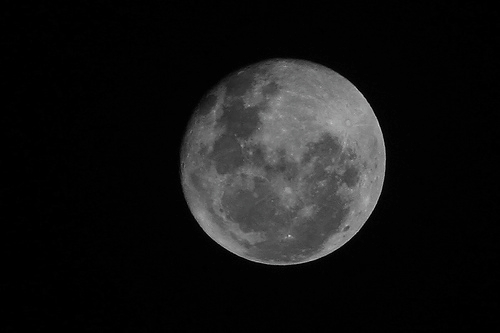
\includegraphics[width=.45\textwidth]{img/unicamp/lua.jpg}
        \end{figure}

    \item  \textbf{Sala 363:} Vulgo salinha de estudo do IC. Pequena e
        aconchegante, tem mesas redondas, muito boas para estudo em grupo. Não
        costuma encher, por isso é bem tranquila. Tem uma estante com vários
        livros doados para uso livre.

    \item  \textbf{Sua casa:} Se você mora em uma república com pessoas da sua
        turma, vá fundo e estude em casa. Se você mora sozinho ou com caras de
        outros cursos/anos, mas se concentra bem em casa, também o faça. Caso
        contrário, estude na Unicamp. É muito fácil se distrair em casa. Você
        vai à geladeira, mexe no computador, lê outra coisa, deita na cama e
        dorme, entre outras coisas. Prefira estudar na Unicamp. Outra coisa, não
        seja egoísta, quando tiver oportunidade de estudar em grupo, prefira
        essa alternativa. Lembre-se que você não está mais no ``cursinho'',
        tente sempre pegar as dicas que a galera te dá, principalmente dos seus
        veteranos.
\end{itemize}

\newpage
%%%%% Melhores banheiros
% Este arquivo .tex será incluído no arquivo .tex principal. Não é preciso
% declarar nenhum cabeçalho

\section{Melhores banheiros}

Uma das maiores necessidades do ser humano pode ser potencializada se for
realizada num banheiro decente. Portanto, é muito importante que você saiba onde
ir. Alguns dos melhores banheiros da Unicamp são:

\begin{itemize}
    \item  \textbf{IC-3:} Geralmente estão limpos e utilizáveis. Mas fedem!
        Sempre com papel higiênico, é uma boa pedida na hora do apuro. Exceto
        nos finais de semana.

    \item  \textbf{IC-2:} Quase sempre estão limpos e utilizáveis e tem um odor
        melhor que os do IC-3. Só precisa tomar cuidado pois, as vezes, falta
        papel higiênico.

    \item  \textbf{FEEC:} Possui excelentes banheiros escondidos por lá. Procure
        bem!

    \item  \textbf{PB:} Os banheiros do segundo e do terceiro andar do Pavilhão
        Básico também são bons (especialmente os do terceiro andar, por quase
        não serem usados). Só tome cuidado, porque às vezes não tem papel
        higiênico.

        \begin{figure}[h!]
            \centering
            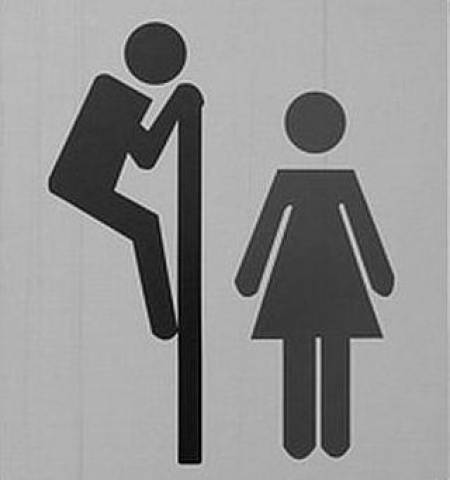
\includegraphics[scale=0.50, keepaspectratio=true]{img/imgs/12-melhores_banheiros/banheiro.jpg}
        \end{figure}

    \item  \textbf{FE:} A faculdade de educação tem poucos banheiros masculinos,
        mas estão entre os melhores da Unicamp pelo pouco uso.

    \item  \textbf{CB:} Estes banheiros ficam escondidos próximo às escadas do
        CB (no térreo). Se você tiver sorte de chegar bem após a limpeza, o
        banheiro estará em excelentes condições. Porém, na maior parte do tempo
        ele fica bem sujinho.

    \item  \textbf{DEQ:} Departamento de Eletrônica Quântica, no IFGW. Dizem que
        ninguém os usa.

    \item  \textbf{DRCC:} Departamento de Raios Cósmicos e Cronologia, no IFGW.
        Um dos melhores banheiros existentes na Unicamp (senão o melhor). Assim
        como os banheiros do DEQ, dizem que ninguém os usa.

    \item  \textbf{DFA:} Departamento de Física Aplicada, no IFGW. Os dois
        andares do departamento tem banheiros bons e utilizáveis, mas algumas
        vezes falta papel higiênico.

    \item  \textbf{IMECC:} Todos os três departamentos (andares) do IMECC tem
        banheiros bons e utilizáveis. Mas vez ou outra falta papel higiênico.
\end{itemize}

\newpage
%%%%% Iniciação Científica
% Este arquivo .tex será incluído no arquivo .tex principal. Não é preciso
% declarar nenhum cabeçalho

\section{Iniciação Científica}

A Iniciação Científica é um tempo para o aluno de graduação (você, no caso) ter
uma experiência acadêmica mais séria, sentir um pouco como é o clima de
pesquisa. Interessou? O que fazer? Calma, você mal entrou na Universidade.
Geralmente, o que se faz é conversar com o professor da área com a qual você se
identifica mais (criptografia, teoria da computação, processamento de imagens,
inteligência artificial etc.) e ver se ele está desenvolvendo algum projeto
interessante naquela área, ou propor para ele alguma ideia sua mesmo.  Depois
você começa a estudar para redigir um projeto e encaminhá-lo para alguma
instituição de fomento à pesquisa (CNPq ou FAPESP), pedindo uma bolsa de
Iniciação Científica. A FAPESP paga em torno de R\$520,00 e aceita pedidos de
bolsa em qualquer período do ano. O CNPq paga aproximadamente R\$400,00, e o
período para inscrição de projetos é geralmente em junho e novembro. No primeiro
semestre geralmente é bem mais difícil achar algum professor da área que você se
interessa, aliás, é bem difícil saber a área com a qual você se identifica, pois
você mal começou o curso e não conhece muito do que se estuda em Computação,
muito menos os professores. Mas tenha paciência, agora parece tudo muito
complicado, mas com o tempo as coisas vão ficando mais simples. Se você
realmente tiver uma sede insaciável de conhecer o meio da pesquisa, procure o
seu professor de MC102, ele pode te orientar a respeito.
\begin{figure}[h!]
    \centering
    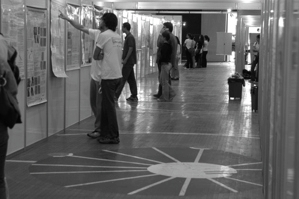
\includegraphics[scale=0.85, keepaspectratio=true]{img/imgs/15-iniciacao/-087.jpg}
    \caption{Congresso de Iniciação Científica da Unicamp}
\end{figure}
Outra coisa interessante a respeito da Iniciação Científica é que, se você
conseguir bolsa (o que não é muito difícil), pode pegar a disciplina MC040 e
posteriormente MC041 (2 semestres), cada uma com 6 créditos, e geralmente se
tira notas altas nessas disciplinas. Ou seja, são 12 créditos praticamente ``de
bandeja'' para aumentar o seu CR, ou ajudar a recuperá-lo, caso esteja no fundo
do poço. Note bem as aspas. Os trabalhos de Iniciação Científica geralmente
consomem muito tempo de estudo e dedicação, não vá pensando que é moleza não.

Na FEEC você pode conseguir as matérias de Iniciação (EA002 até EA005) mesmo sem
bolsa, mas você ainda assim vai precisar de um orientador. Lá a Iniciação
Científica também substitui o estágio, mas não tem equivalência com as do IC.

\newpage
%%%%% Acesso a artigos e revistas científicas
% Este arquivo .tex será incluído no arquivo .tex principal. Não é preciso
% declarar nenhum cabeçalho

\section{Acesso a artigos e revistas científicas}

Os resultados de pesquisas científicas, no Brasil e no mundo todo, costumam ser
publicados por meio de periódicos e conferências, os quais normalmente são
disponíveis pela internet.

No Brasil, quase todas as instituições públicas de ensino superior, como a
Unicamp, participam de um sistema conhecido como \textbf{Portal de Periódicos da
Capes} (\url{periodicos.capes.gov.br}), que garante acesso a grande parte das
publicações científicas das principais editoras do mundo sem necessidade de
pagar nada a mais por isso.

Nas áreas de engenharia e de computação, quase todas as publicações relevantes
são acessíveis através desse sistema. Mas é importante você saber que esse tipo
de acesso só é possível a partir de endereços IP da Universidade, então se você
quiser acessar algum artigo quando estiver em casa, o ideal é usar o sistema de
acesso VPN (Virtual Private Network) disponibilizado pela Unicamp, como pode ser
visto no site: \url{www.ccuec.unicamp.br/ccuec/acesso_remoto_vpn}.

Através da \textbf{Comunidade Acadêmica Federada (CAFe)}, foi disponibilizado
recentemente um método de acesso remoto aos periódicos sem necessidade de usar a
VPN, mais informações aqui: \url{www.ccuec.unicamp.br/biti/download/instrucoes_acesso_CAFe.pdf}

Na Unicamp, você ainda tem acesso a diversas outras publicações e e-books que
não são cobertos pelo sistema da Capes, além de alguns periódicos impressos, que
podem ser encontrados nas bibliotecas. Caso você queira buscar algo no material
que há disponível física ou virtualmente na Universidade, acesse o site do
\textbf{Sistema de Bibliotecas da Unicamp}: \url{www.sbu.unicamp.br}.

Para uma busca mais abrangente de artigos científicos na internet, você pode
usar o \textbf{Google Acadêmico} (\url{scholar.google.com}). Mas atenção! Você
pode encontrar artigos que não são cobertos pelo Portal da Capes nem pela
Unicamp e exigem pagamento.

Além do Portal de Periódicos, existe também um novo modelo de publicações
científicas de acesso gratuito, chamado \textbf{open access}. Esse modelo tem
origem muito próxima do movimento pelo software livre. Publicações feitas nesse
sistema são acessíveis a qualquer momento, de qualquer IP e sem qualquer custo.
Alguns exemplos de grandes repositórios e editoras open access são:

\begin{itemize}
    \item  \textbf{SciELO:} \url{www.scielo.org}
    \item  \textbf{PLOS:} \url{plos.org}
    \item  \textbf{arXiv:} \url{arxiv.org}
    \item  \textbf{PMC:} \url{ncbi.nlm.nih.gov/pmc}
\end{itemize}

A rede \textbf{SciELO} é onde a maior parte dos artigos em português é
publicada. O acervo \textbf{PMC} é de publicações da área biomédica.

Bixo, guarde bem esta seção do Manual! Pode ser que você não vá usá-la logo de
cara, mas quando você fizer iniciação científica ou um trabalho de disciplinas
mais avançadas, você aproveitará bastante essas informações.

\newpage
%%%%% Intercâmbio
% Este arquivo .tex será incluído no arquivo .tex principal. Não é preciso
% declarar nenhum cabeçalho

\section{Intercâmbio}

A Unicamp é uma das universidades brasileiras que têm maior prestígio fora do
país e a VRERI-Unicamp (Vice-Reitoria Executiva de Relações Internacionais,
antigo CORI), IC e FEEC têm vários acordos bilaterais de intercâmbio. Então,
para você que quer dar um salto em algum idioma, conheceroutras culturas e
sentir na pele a aventura de ser estrangeiro, comece a se preparar desde já.
nnn
A França hoje recebe grande número de estudantes de computação, devido a acordos
que a FEEC tem com os INSA e com as Écoles Centrales e também graças a bolsas de
estudo oferecidas pela Capes e pelo governo francês. Mas não significa que a
França seja seu destino certo: no site da VRERI existem oportunidades para ir
para Estados Unidos, Japão, América Latina, Alemanha, Espanha etc., muitos com
boas bolsas de estudo ou com incentivos que valem a pena caso você tenha um
pouco de grana para se sustentar no início. Visite sempre o site da VRERI e
participe das reuniões que ela faz, pois ficar ligado é a chave para conseguir
encontrar uma boa oportunidade. Existem outras opções de intercâmbio, como a
AIESEC, que promove um intercâmbio para estágios no exterior. Se seu interesse é
mais profissional, procure se informar.

Fique de olho também no programa Ciência sem Fronteiras, do governo federal, que
desde o ano passado distribui bolsas para instituições de excelência dos Estados
Unidos, Alemanha, Itália, Reino Unido, entre outros.

``Mas vale a pena? Poxa, vou atrasar meu curso, ficarei deslocado de turma, vou
ficar em um país estranho, para quê? Acho que não vale a pena{\dots}''

Vamos começar pelos motivos profissionais: ter no currículo que você fala uma
língua estrangeira fluentemente devido à sua imersão no país é algo muito
valorizado pelas empresas, além do fato que o pessoal do RH vai ver que você tem
capacidade de se virar sozinho, uma vez que não é tão óbvio sair do país e
recomeçar sua vida fora. Você não atrasará tanto seu curso, pois a Unicamp conta
com um sistema de equivalências de matérias, e se você escolher bem pode fazer
matérias que serão convalidadas na Unicamp. Agora, o que realmente é importante:
você está na faculdade, está na hora de deixar o colo da mamãe e partir para o
mundo! A experiência de conhecer outras culturas, criar laços de amizade
internacionais, viajar por terras desconhecidas não tem preço! Pense que é no
seu tempo de facul que terá oportunidade de fazer uma aventura destas, não
desperdice.

Se você abriu um sorriso e pensa que está preparado para sair do país, comece a
estudar, bixo! Não que ter uma boa nota seja a única forma de conseguir uma vaga
em uma bolsa de estudos, mas com certeza é a mais fácil.  Busque atirar em todas
as frentes, mantenha seu CR num bom nível, busque conhecer organismos como
AIESEC e procure grupos de trabalho (no IC existem vários) que podem levar
alunos ao exterior. Boa sorte!

Se você realmente se interessou, aí vão uns links com mais informações:

\begin{itemize}
    \item  VRERI: \url{www.internationaloffice.unicamp.br}
    \item  AIESEC: \url{aiesec.org.br}
    \item  Ciência sem Fronteiras: \url{cienciasemfronteiras.gov.br}
    \item  Site da Pró-reitoria de graduação sobre o CsF: \url{www.prg.unicamp.br/csf}
\end{itemize}

Fique atento aos e-mails que você receberá do IC e da FEEC. Muitos deles são
sobre programas de intercâmbio.

\newpage
%%%%% Cuidado com CR e Reprovação
% Este arquivo .tex será incluído no arquivo .tex principal. Não é preciso
% declarar nenhum cabeçalho

\section{Cuidado com CR e Reprovação}

Durante o curso você vai ouvir que se preocupar com seu CR é bobagem, que
estudar para tirar nota não leva a lugar nenhum, que depois de formado não é seu
CR que te colocará no mercado de trabalho, etc. Cuidado, trabalhar numa empresa
não é a sua única opção de vida após formado, e preste atenção, pois ``após
formado'' não significa durante o curso.

Durante o curso você vai ter a possibilidade de participar de várias atividades
acadêmicas e algumas delas vão exigir bom aproveitamento acadêmico do aluno. Por
exemplo, para se candidatar a monitor de uma disciplina é exigido do aluno um CR
pelo menos 0,7. Isto significa que sua média de notas das disciplinas cursadas
até aquele momento deve ser maior ou igual a 7,0. Para pleitear uma bolsa de
iniciação científica, onde há concorrência entre alunos do país todo, também
será exigido bom aproveitamento, assim como para uma bolsa de mestrado. Caso
você não saiba, mestrado faz parte da pós-graduação, ou seja, o seu CR vai te
influenciar até após formado.

Cuidado também com a reprovação. Há instituições, como a FAPESP (Fundação de
Amparo à Pesquisa do Estado de São Paulo), que é a maior fomentadora de
pesquisas do estado de São Paulo e que paga os maiores valores de bolsas do
país, que te excluem de qualquer disputa só por ter uma reprovação no seu
histórico escolar da graduação. Não te exclui oficialmente, mas como é muito
concorrido por ser a melhor pagadora, se seu nome for para o final da lista por
causa da reprovação pode considerar-se excluído da disputa.

Parece óbvio que quem estuda tira boas notas, mas até você aprender a estudar
como a universidade exige, pode demorar um pouco, e há pessoas que nunca
aprendem.

Há certos períodos (semestres) quando você já estiver mais avançado no curso em
que poderá sentir-se à vontade para desistir de uma disciplina em que esteja
matriculado, deixando para completá-la posteriormente. Quando você fizer isso há
a possibilidade de desistir da disciplina, desmatriculando-se oficialmente dela.
Mas há pessoas que simplesmente deixam de cursar a disciplina, reprovando por
nota e falta e ficando com uma nota baixa em seu histórico. Cuidado com isso,
pode ser frustrante para você no futuro. Por isso, se for desistir de cursar uma
disciplina após matriculado, sempre peça a desistência e tente não reprovar.

Lembre-se de que 4 ou 5 anos é muito tempo, você pode mudar de ideia a qualquer
momento sobre o que pretende fazer no futuro.

\newpage
%%%%% Pra que que eu estou estudando isso??
% Este arquivo .tex será incluído no arquivo .tex principal. Não é preciso
% declarar nenhum cabeçalho

\section{Para que eu estou estudando isso?}

O ensino médio acabou, você finalmente está livre de todas as inutilidades, como
química orgânica e separação silábica de verbos parnasianos, só vai ver coisas
relevantes para a profissão, e{\dots}

Pimba! HZ291. Pode, Arnaldo?

Primeiro, você precisa saber que a Universidade não é um curso técnico. A ideia
não é só te dar capacitação profissional, mas sim formar pessoas melhores. Para
que um computeiro precisa de contabilidade? Para nada, mas uma pessoa (de exatas
pelo menos) precisa ter uma noção disso.

Outro problema: o que exatamente é ``relevante para a sua profissão''?  A
computação é uma área muito vasta, e a graduação é bem generalista, para te dar
base para escolher. Por exemplo, vai ter gente que nunca mais vai usar
GA/Algelin, mas quem for para a área de computação gráfica vai comer matriz no
café da manhã. Quem garante que no meio do curso você não decida ir para essa
área? Ou ainda, que no seu emprego não te joguem um problema desse tipo?

Se você continuar na Universidade, na pós você só terá matérias da sua área, já
que você já sabe o suficiente pra dizer que área é essa. Mas ainda falta muito
chão até lá{\dots}

Para quem é da Engenharia, um problema maior é que, para conseguir o CREA,
existem algumas matérias obrigatórias (embora completamente inúteis, sem
exagero), como Resistência dos Materiais. A Unicamp pode até contrariar essas
orientações, até certo ponto, mas dificilmente os professores concordariam. (Por
outro lado, você poderá construir prédios de até 2 andares. Recomendamos
fortemente que você não faça isso.)

Para quem é da Ciência, o curso não é para formar simples programadores. Vocês
serão mais que isso, serão cientistas, e isso envolve ver coisas além de só
código.


\chapter{Além da graduação}
%%%%% Grupos e Entidades da Unicamp
% Este arquivo .tex será incluído no arquivo .tex principal. Não é preciso
% declarar nenhum cabeçalho

\section{Grupos e Entidades da Unicamp}

\subsection{Alumni Computação Unicamp}

\begin{figure}[H]
    \centering
    
\includegraphics[scale=0.40]{img/alem_da_graduacao/alumni_logo.png}
\end{figure}

Alumni é o nome dado a ex-alunos de uma universidade. Por extensão, alumni
também é o nome de organizações sem fins lucrativos motivadas em manter o
relacionamento entre a universidade e os ex-alunos e o destes entre si, servindo
como uma rede de contatos profissionais. A comunicação entre alunos, ex-alunos e
professores proporciona um compartilhamento de experiência e informações, que
contribuem para uma diferenciação acadêmica, cultural e profissional.

O \textbf{Alumni Computação Unicamp} é uma forma de manter todos que passaram
pelo melhor curso de computação da América Latina conectados -- tanto alunos
quanto ex-alunos. Atualmente o Alumni conta com uma página no Facebook
(\url{fb.com/AlumniComputacaoUnicamp}), que reúne os grupos das turmas que
passaram pela Computação, com o objetivo de atingir o maior número de alunos e
ex-alunos.

Participe do grupo de sua turma, convide seus amigos a curtirem a página, envie
sugestões e contribua para essa ideia!

\subsection{ARU}

\subsubsection*{O que é a ARU – Associação de Repúblicas da Unicamp?}

\begin{figure}[H]
    \centering
    
\includegraphics[scale=0.40]{img/alem_da_graduacao/aru_logo.png}
\end{figure}

Idealizada em 2008, a ARU é a entidade que representa as Repúblicas Associadas
de Barão Geraldo.  Tem como meta prestar apoio a elas, zelar pela sua segurança
e bem estar com toda a vizinhança, como também servir de espaço para discutir os
problemas apresentados em reuniões.

\begin{figure}[H]
    \centering
    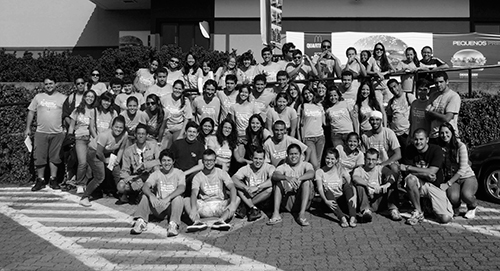
\includegraphics[scale=0.40]{img/alem_da_graduacao/aru_foto.jpg}
\end{figure}

Além de entregar no começo do ano um manual para os bixos contendo informações
sobre as Repúblicas Associadas, a ARU também realiza vários eventos, os quais
têm o objetivo de integrar e divertir os moradores de repúblicas. Alguns deles
são: a \textbf{Alcorrida}, a \textbf{Campanha do Agasalho}, o
\textbf{EntortaRep}, e, principalmente, o \textbf{InterReps}.

\subsubsection*{Contato}

\begin{compactitemize}
    \item Site: \url{republicasunicamp.com.br}
    \item E-mail: \email{contato@republicasunicamp.com.br}
    \item Facebook: \url{fb.com/republicasunicamp}
\end{compactitemize}

\subsection{Competições de programação}

Curte programar? Nunca programou mas está gostando de MC102? Já brincou de
Olimpíada naquelas provas com direito a medalha? Vá fundo!

Para os bixos que ingressaram direto do ensino médio existe a \textbf{OBI --
Olimpíada Brasileira de Informática}, logo no primeiro semestre.  Anualmente,
muitos alunos do IC, tanto da Ciência como da Engenharia, ganham premiações
nessa competição. O site dela é \url{olimpiada.ic.unicamp.br}.  Visite-o para
mais informações.

\begin{figure}[h!]
    \centering
    
\includegraphics[scale=0.40]{img/alem_da_graduacao/maratona_logo.png}
\end{figure}

Mas a principal competição para alunos de ensino superior é a \textbf{Maratona
de Programação}, que consiste de problemas mais difíceis e é feita em equipes de
três alunos. A Unicamp tem grande tradição nessa competição, tendo levado
equipes para a competição mundial (a ACM-ICPC) em 1996, 2000, 2002, 2003, 2004,
2007, 2009 e 2012.

Além de brilhar no currículo, é muito divertido competir, e a experiência obtida
nos treinamentos tem levado muitos maratonistas a empresas como Google,
Microsoft e Facebook.

Para participar dos treinamentos para a Maratona que acontecem na Unicamp,
inscreva-se no grupo \url{groups.google.com/group/maratona_unicamp}.

\subsection{DCE}

Criado em 1978, o DCE Unicamp (Diretório Central dos Estudantes) é a entidade
que representa todos os estudantes de graduação da Universidade, articulando e
organizando o movimento estudantil (ME).

Cabe ao DCE representar o conjunto dos estudantes em todos os espaços dentro e
fora da universidade, diante das mais diversas entidades (reitoria, sindicatos,
DCEs de outras universidades, centros acadêmicos, associações etc.) e movimentos
sociais.

Como articulador do ME, cabe ao DCE organizar os estudantes na luta por uma
educação superior realmente pública, gratuita e de qualidade. Para tanto, é
papel fundamental do DCE propor, juntamente com os centros acadêmicos,
discussões políticas que extrapolem os nossos currículos e o nosso dia a dia.
Além disso, o DCE deve propor ações que vão ao encontro das reivindicações
estudantis, de forma que elas sejam levadas e cobradas da reitoria ou até mesmo
do governo.

O DCE esteve envolvido em várias conquistas dos estudantes, das quais se
destacam algumas lutas históricas: a construção da moradia estudantil; a
melhoria de estrutura para cursos noturnos, que tornou acessível para esse
período bibliotecas, xérox, laboratórios e secretarias de graduação; a reunião
semestral para avaliação de curso; o não-aumento do preço do bandejão; uma
seleção mais justa para as vagas na moradia; entre diversas outras. Além disso,
o DCE teve participação em importantes lutas sociais que extrapolam o âmbito da
Unicamp, como a organização do Plebiscito contra a Alca e do Plebiscito contra o
Provão; a luta por mais verbas para a educação no estado de São Paulo; diversas
lutas pela qualidade do ensino e manutenção de direitos dos estudantes em outras
universidades como na UNIP, UNIMEP, FUPPESP etc.

No fim do ano, há eleições para definir qual a chapa que comandará a entidade no
ano seguinte, juntamente com eleições para representação discente no Consu e na
CCG. É muito importante a participação dos alunos nessas eleições.

Não deixe de participar da Calourada Integrada organizada pelo DCE e centros
acadêmicos e das reuniões do DCE, que acontecem na sede próxima ao Bandejão.

\begin{compactitemize}
    \item  Telefone: (19) 3521-7910 / (19) 3521-7042
    \item  E-mail: \email{dceunicamp@gmail.com}
    \item  Site: \url{dceunicamp.org.br}
\end{compactitemize}

\subsection{Equipe Phoenix}

\begin{figure}[h!]
    \centering
    
\includegraphics[width=.35\textwidth]{img/alem_da_graduacao/phoenix_logo.jpg}
\end{figure}

A Equipe Phoenix de Robótica da Unicamp é composta por alunos da Mecânica,
Elétrica e Computação, e desenvolve projetos todo ano para participar de
competições nacionais como a RoboCore, disputando pela categoria de melhor robô
de combate, sumô, trekking e seguidor de linha, entre outros.

Para aqueles interessados pela programação um robô, pela eletrônica das placas
de controle ou ainda pela mecânica dos robôs que resistem a impactos gigantescos
durante a guerra, a equipe realiza um processo seletivo todo começo de ano, com
inscrições através do site. Se envolva!

\begin{compactitemize}
    \item  Site: \url{phoenixunicamp.com.br}
    \item  Facebook: \url{fb.com/phoenixunicamp}
\end{compactitemize}

\subsection{Gamux}

O Gamux (Grupo de Pesquisa e Desenvolvimento de Jogos da Unicamp), composto por
computeiros e alunos do IA (Instituto de Artes), é uma ótima oportunidade para
quem tiver curiosidade de saber como são feitos os jogos eletrônicos.

Fique atento, eles costumam organizar ciclos de palestras e eventos relacionados
a desenvolvimento de jogos.

Mas não precisa esperar até lá! Apareça no LMS (Laboratório da Microsoft,
próximo as mesinhas do IC3) ou entre no grupo de e-mail.

\begin{compactitemize}
    \item  Site: \url{gamux.com.br}
    \item  Lista de discussão: \url{groups.google.com/group/gamedev_unicamp}
\end{compactitemize}

\subsection{GPSL}

O \textbf{GPSL -- Grupo Pró Software Livre} é aberto para alunos de todas as
unidades e para a comunidade. Sua missão é promover o uso e o desenvolvimento do
software livre.

Muitas instituições educacionais utilizam software proprietário e a Unicamp não
é exceção. São poucas as unidades que usam software livre e é muito fácil se
formar sem sequer saber da existência ou ter qualquer experiência com algo
diferente do software proprietário vigente.

\begin{figure}[h!]
    \centering
    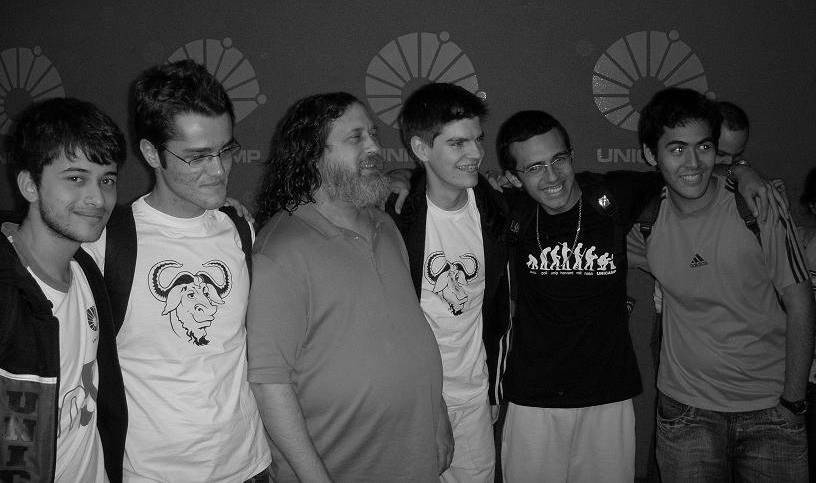
\includegraphics[scale=0.36]{img/alem_da_graduacao/gpsl_foto.jpg}
    \caption{Richard Stallman em vista à Unicamp}
\end{figure}

O GPSL é um espaço para refletir sobre a predominância do software proprietário,
cujo uso muitas vezes é imposto, inclusive pela universidade, a ética por trás
disso e os efeitos sociais decorrentes. É também um espaço para se articular e
pensar em formas de ação, que podem envolver desde a educação e a
conscientização dos usuários de computadores até o próprio desenvolvimento de
software livre. O GPSL também pensa sobre questões de mercado e econômicas
relacionadas ao software livre.

Tradicionalmente, o GPSL organiza, com o apoio do CACo, o \textbf{Curso de
GNU/Linux Para os Bixos}. Este curso, como o próprio nome diz, é voltado para os
bixos como você que ingressam nos cursos de computação, embora seja aberto
também a veteranos. O objetivo é ensinar o básico do sistema operacional
GNU/Linux para você se virar nas matérias de computação do primeiro semestre.
Ele geralmente é ministrado em abril, mas não existe data fixa. Mas não se
preocupe, você será avisado na sala de aula por um veterano e receberá um
comunicado pelo seu e-mail do IC.

Para participar das discussões do GPSL, inscreva-se no grupo de e-mail em
\url{groups.google.com/group/gpsl-unicamp}.

\subsection{MTE}

\begin{figure}[H]
    \centering
    
\includegraphics[scale=0.40]{img/alem_da_graduacao/mte_logo.png}
\end{figure}

O \textbf{MTE -- Mercado de Trabalho em Engenharia} é uma entidade estudantil
que visa colocar o aluno da Unicamp em contato mais próximo com o mercado de
trabalho e com as possibilidades que ele proporciona, mostrando as diferentes
áreas de atuação de um engenheiro.

A participação no MTE desenvolve habilidades como networking, oratória,
expressão, empreendedorismo, gestão e diversas outras.

A estrutura do MTE é dividida em três pilares:

\begin{description}
    \item[Oportunidades:] responsável por atividades como visitas técnicas e
        captação de treinamentos e palestras.

    \item[Desenvolvimento:] responsável por atividades como English Meeting
        (encontros de conversação em inglês), Teia do Conhecimento (treinamentos
        dados por algum dos membros) e Ciclo de Oratória (ciclos com foco em
        melhoria de expressão).

    \item[Orientação e Carreira:] responsável pela estruturação pessoal e
        profissional dos membros realizando feedbacks, atividades de
        consultoria, de motivação, entrevista com profissionais e
        confraternizações.
\end{description}

Além da participação em um dos pilares, alguns membros participam da diretoria
administrativo-financeira e, para completar, participam da realização de dois
principais eventos: o EMC (Estudante e Mercado Conectados) que conta com visitas
técnicas e palestras e o ArenaMTE, um desafio universitário de resolução de
cases.

Para mais informações sobre o MTE e seu processo seletivo, acesse
\url{mte.org.br}.

\subsection{Rádio Muda}

Você provavelmente nunca viu nada do tipo na sua vida. Uma rádio na qual
qualquer ser humano pode fazer o seu programa tranquilamente, sem burocracias
(tendo espaço na grade de horários, lógico).

A Rádio Muda fica embaixo da caixa d'água (carinhosamente apelidada de Pau do
Zeferino) que fica perto do Teatro de Arena, bem em frente à BC (Biblioteca
Central).

Se você só quiser ouvir a muda, 88,5 MHz no seu rádio (em Barão Geraldo ou
Paulínia) ou pela Internet, através do site \url{muda.radiolivre.org}.

\subsection{Curso Exato}

O Curso Exato é um projeto da Pró-Reitoria de Extensão e Assuntos Comunitários
da Unicamp criado em 2008 por alunos de graduação, com a finalidade de explorar
o potencial e a capacidade dos alunos de se expressarem, de raciocinarem
logicamente e de compreenderem o mundo que os cerca, por meio de aulas de Língua
Portuguesa, Matemática, Física e Química.

Os professores do curso são alunos de graduação e pós-graduação da universidade
e o público alvo é constituído por alunos da rede pública de ensino com
disposição e interesse para aprender.

As aulas são realizadas no período noturno, das 19h15 às 22h30, de segunda a
quinta-feira, no campus da universidade.

\begin{compactitemize}
    \item Site: \url{cursoexato.com.br}
    \item Facebook: \url{fb.com/curso.exato}
    \item E-mail: \email{curso.exato@gmail.com}
\end{compactitemize}

\subsection{Grupos Religiosos}

\subsubsection*{ABU -- Aliança Bíblica Universitária}

Grupo evangélico não ligado a nenhuma denominação, organiza várias reuniões e
grupos de discussões e é filiado à Aliança Bíblica Universitária do Brasil
(\url{abub.org.br}).

\begin{compactitemize}
    \item Site: \url{abucampinas.org}
    \item E-mail: \email{contato@abucampinas.org} ou
        \email{abucamp_co@yahoogrupos.com.br}
    \item Telefone: (19) 3289-2823
\end{compactitemize}

\subsubsection*{Pastoral Universitária}

Grupo católico que se reúne semanalmente para estudar textos (bíblicos ou não),
livros, documentos, aprofundar a fé e promover a integração e união de seus
participantes. A Pastoral Universitária também organiza grupos de preparação
para Primeira Comunhão e Crisma, além de duas Missas semanais e Grupos de Oração
Universitários (GOUs). As Missas são realizadas às terças (18h) e às quintas
(12h15), sempre no PB04. Os GOUs acontecem às terças (12h15) e nas quintas
(18h), também no PB04.

\begin{compactitemize}
    \item Site: \url{sites.google.com/site/pastoralunicamp}
    \item E-mail: \email{pastoralunicamp@gmail.com}
\end{compactitemize}

\newpage
%%%%% Conpec
% Este arquivo .tex será incluído no arquivo .tex principal. Não é preciso
% declarar nenhum cabeçalho

\section{Conpec}

\begin{figure}[H]
    \centering
    
\includegraphics[scale=0.40]{img/conpec.png}
\end{figure}

A Conpec é a empresa júnior dos cursos de Ciência e Engenharia de Computação da
Unicamp.

Nela você tem a oportunidade de aplicar os conhecimentos teóricos adquiridos em
sua vida acadêmica em uma situação real, de mercado, com clientes, prazos e
soluções reais. É uma chance ainda de aprender sobre aspectos de mercado de
trabalho que você nunca veria na faculdade, como marketing, finanças,
planejamento, trabalho em equipe e liderança, indispensáveis considerando-se que
o perfil empreendedor é cada vez mais exigido do profissional de computação.
Muitos membros e ex-membros da Conpec usam os conhecimentos adquiridos na
empresa não só como um adicional ao buscar uma vaga no mercado de trabalho, mas
também para montar suas próprias empresas ou em serviços não ligados diretamente
à computação, como consultorias estratégicas.

Além disso, a Conpec é uma excelente oportunidade para conhecer os seus colegas
de curso, sejam veteranos ou bixos, pessoas de outros cursos e até mesmo de fora
da Unicamp, uma vez que há diversas empresas juniores espalhadas pelas
universidades de São Paulo e do Brasil. É ainda uma grande chance para perder a
inibição de falar em público e aperfeiçoar sua capacidade de expor opiniões,
além de aprender como agir em um ambiente profissional.

\begin{figure}[H]
    \centering
    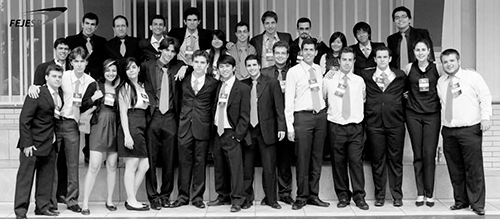
\includegraphics[scale=0.40]{img/conpec_foto.jpg}
\end{figure}

Para fazer parte da Conpec, fique atento à data da palestra de apresentação do
processo seletivo, que ocorre no início do ano.

Para saber mais sobre a empresa visite o site \url{conpec.com.br} ou tire suas
dúvidas mandando um e-mail para \email{conpec@conpec.com.br}.

\newpage
%%%%% Atlética -- AAACEC
% Este arquivo .tex será incluído no arquivo .tex principal. Não é preciso
% declarar nenhum cabeçalho

\section{Atlética -- AAACEC}

A \textbf{AAACEC -- Associação Atlética Acadêmica da Ciência e Engenharia de
Computação}, ou simplesmente \textbf{Atlética}, é a entidade estudantil que
promove a prática de esportes na Computação.

Uma entidade sem fins lucrativos, a AAACEC tem sua diretoria eleita anualmente
pel*s alun*s associad*s dos cursos de Engenharia e Ciência da Computação e da
pós-graduação no IC.

A Atlética é responsável pela participação da Computação em competições
esportivas, tanto dentro da Unicamp (Calouríadas, Interanos, Olimpíadas) quanto
fora (Intercomp).

\begin{figure}[H]
    \centering
    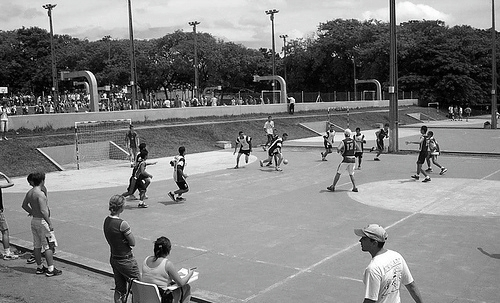
\includegraphics[scale=0.55]{img/alem_da_graduacao/aaacec_foto.jpg}
\end{figure}

A fim de possibilitar essa participação, a AAACEC promove treinos regulares de
basquete, vôlei, handebol e futsal e disponibiliza o material (bolas, redes
etc.) para a prática de tais esportes. A AAACEC se encarrega da reserva de
quadras para a realização dos treinos e competições em que isso se fizer
necessário. Os treinos são semanais e oferecidos para as modalidades masculina e
feminina, de forma que qualquer associad* da Atlética pode participar.

Para associar-se à AAACEC, *s ingressantes podem comprar o \textbf{Kit Bixo},
que contém produtos como camiseta, caneca, mouse pad e chaveiro. Veteran*s podem
associar-se mediante o pagamento de uma taxa. Além do Kit Bix*, a AAACEC vende
outros produtos, como agasalhos.

Além de promover a prática esportiva, a Atlética também realiza festas e eventos
de integração, como a tradicional \textbf{Choppada da Computação} no começo do
ano (gratuita para bix*s, não perca!).

Para saber mais sobre a Atlética e como participar, entre em contato por:

\begin{compactitemize}
\item  E-mail: \email{aaacec@gmail.com}
\item  Site: \url{aaacec.com}
\end{compactitemize}

\subsection{Bateria Valorosa}

\begin{figure}[H]
    \centering
    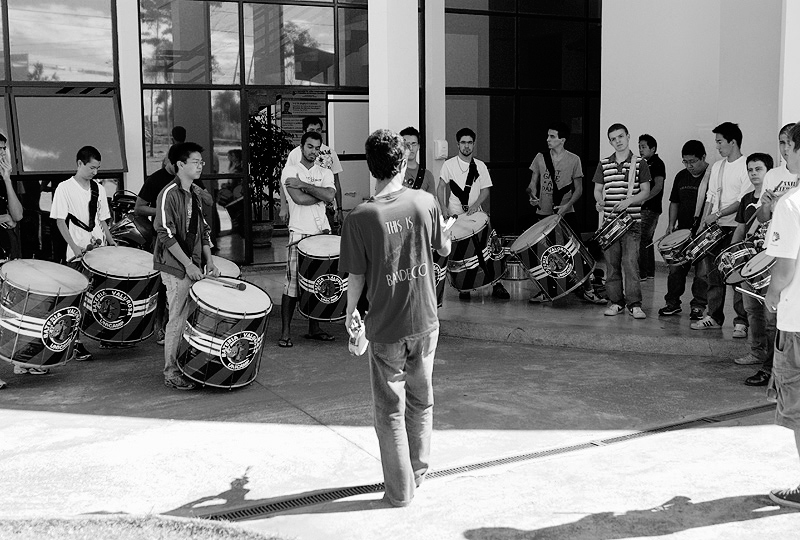
\includegraphics[scale=0.27]{img/alem_da_graduacao/valorosa_foto1.jpg}
\end{figure}

Criada em 1998 e filiada à AAACEC, a \textbf{Bateria Valorosa} é umas das
melhores baterias universitárias da Unicamp. Você muito provavelmente vai
conhecê-la no primeiro dia de aula.

Ao longo do ano, a Valorosa toca em diversos eventos, como o Intercomp, o
Interbatuc e a UPA. A Bateria toca também em festas e para apoiar *s atletas em
jogos internos da Computação e de outros cursos.

A Valorosa realiza ensaios semanais, dos quais estão tod*s, especialmente bix*s,
convidados a participar. Basta comparecer aos ensaios, não é necessário saber
tocar nenhum instrumento. Tod*s que quiserem aprender são muito bem-vind*s na
bateria!

Para mais informações sobre a Bateria Valorosa, acesse o site da AAACEC.

\begin{figure}[H]
    \centering
    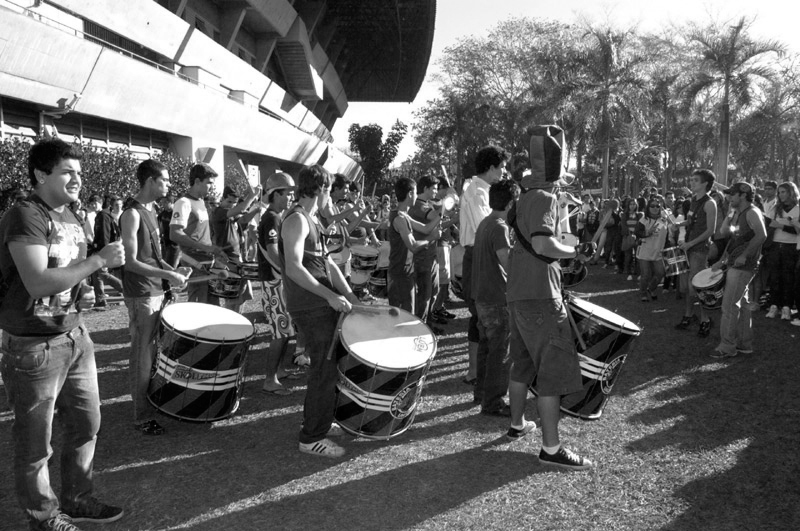
\includegraphics[scale=0.27]{img/alem_da_graduacao/valorosa_foto2.jpg}
\end{figure}

\newpage
%%%%% Centro Acadêmico da Computação
% Este arquivo .tex será incluído no arquivo .tex principal. Não é preciso
% declarar nenhum cabeçalho

\section{CACo -- Centro Acadêmico da Computação}

\begin{figure}[H]
    \centering
    
\includegraphics[width=.35\textwidth]{img/caco_logo.pdf}
\end{figure}

Bixo, o CACo é o seu centro acadêmico. Um CA é uma entidade estudantil que, em
linhas gerais, deve trabalhar para garantir os interesses dos estudantes e
melhorar o curso e a faculdade a que pertence. O CACo é formado pelos alunos de
graduação tanto em Engenharia quanto em Ciência da Computação da Unicamp, bem
como os alunos de pós-graduação do IC. Todo e qualquer aluno desses cursos é
membro do CACo e isso inclui você.

Um centro acadêmico é parte do famoso ``movimento estudantil'' de que você
provavelmente já ouviu falar. Mas não se engane! Pergunte para o seu pai o que
ele pensa quando lê ``movimento estudantil'' e ele vai dizer que vê um bando de
estudantes desocupados associados a um partido político de esquerda que saem por
aí protestando contra o sistema e queimando ônibus pelas ruas. Se você pensa
assim, mude sua ideia: o CACo não é nada disso.

\begin{figure}[H]
    \centering
    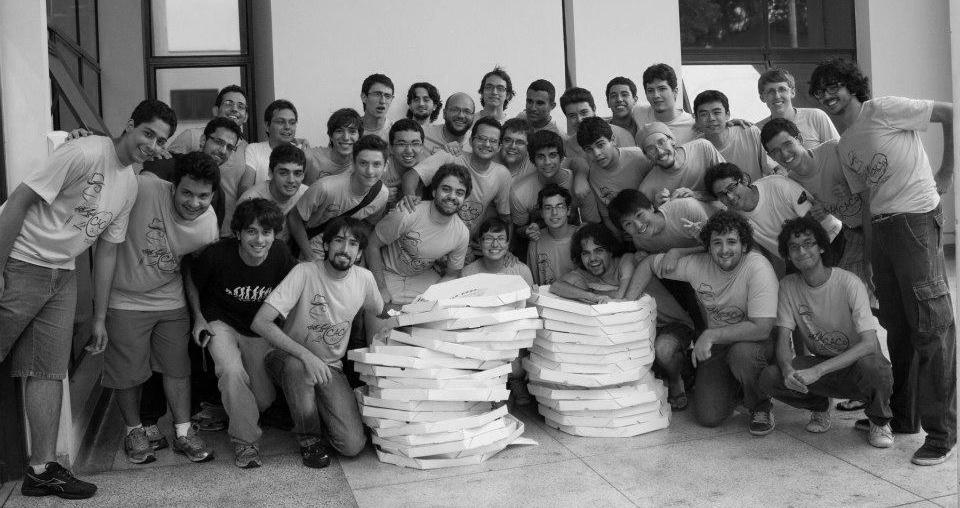
\includegraphics[width=.45\textwidth]{img/alem_da_graduacao/caco_pizzada1.jpg}
\end{figure}

O CACo tem como função representar os estudantes no âmbito acadêmico, ou seja,
perante o IC, a FEEC e a Unicamp. Mas o que o CACo faz? De forma simplificada,
procuramos ser porta-voz dos alunos. Reivindicamos espaço físico decente para os
alunos, alteração nas matérias e professores, promovemos discussões sobre temas
polêmicos e delicados, dentre muitas outras atividades.

Quer um exemplo? Esse estupendo manual que você está lendo neste exato momento
foi confeccionado pelo seu centro acadêmico para lhe ajudar no início da sua
vida universitária e, na verdade, você ainda vai se pegar recorrendo ao seu
Manual várias vezes durante seus quatro, cinco, doze anos na Unicamp.

Uma grande função do CACo é prezar pela qualidade dos cursos e fazemos isso, por
exemplo, através de discussões com o próprio Instituto, onde levamos reclamações
e reivindicações dos alunos para os coordenadores e professores.

\begin{figure}[H]
    \centering
    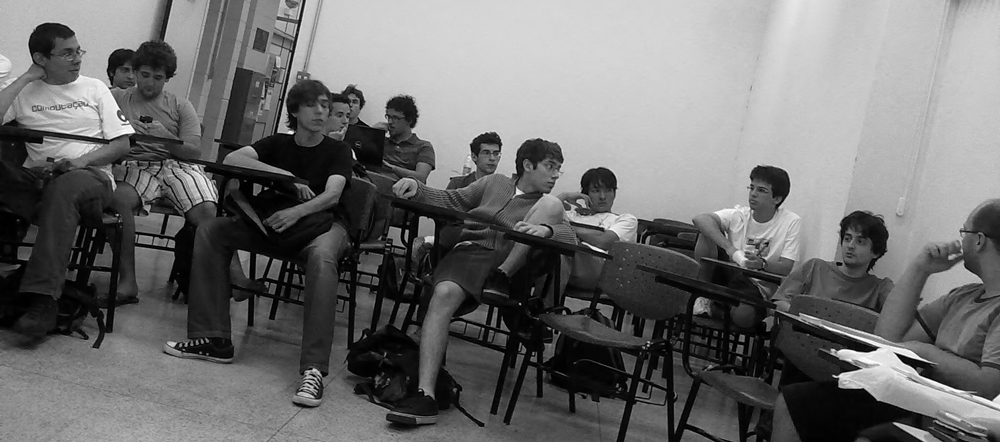
\includegraphics[width=.45\textwidth]{img/alem_da_graduacao/caco_reuniao.jpg}
\end{figure}

Uma outra função do CACo é integrar os estudantes de computação da Unicamp. Para
isso, realizamos diversos eventos como o CineCACo, o PipoCACo, o CACo Games, o
CACo Series of Poker e a grande comemoração do Aniversário do CACo, que contou
com pizza de graça para mais de duzentos alunos! Tentamos também facilitar a
vida da galera através dos armários que alugamos, o Banco de Livros e o Banco de
Provas, o maior da Unicamp, disponível online.

Repetindo o que foi dito antes: bixo, o CACo é o \textbf{seu} Centro Acadêmico.
Tudo que dissemos que fazemos pelos alunos, queremos fazer por você também. Por
isso, quando houver algum problema envolvendo a FEEC, o IC, os professores ou
qualquer coisa do tipo, não hesite em nos procurar. O CACo sempre lhe dará todo
o suporte necessário. Se tiver reclamação ou sugestão relacionada ao próprio
CACo, também estaremos aqui para ouvir. Mais do que isso, venha participar de
uma de nossas reuniões, que são abertas a você e todos os alunos de computação
da Unicamp.

\begin{figure}[H]
    \centering
    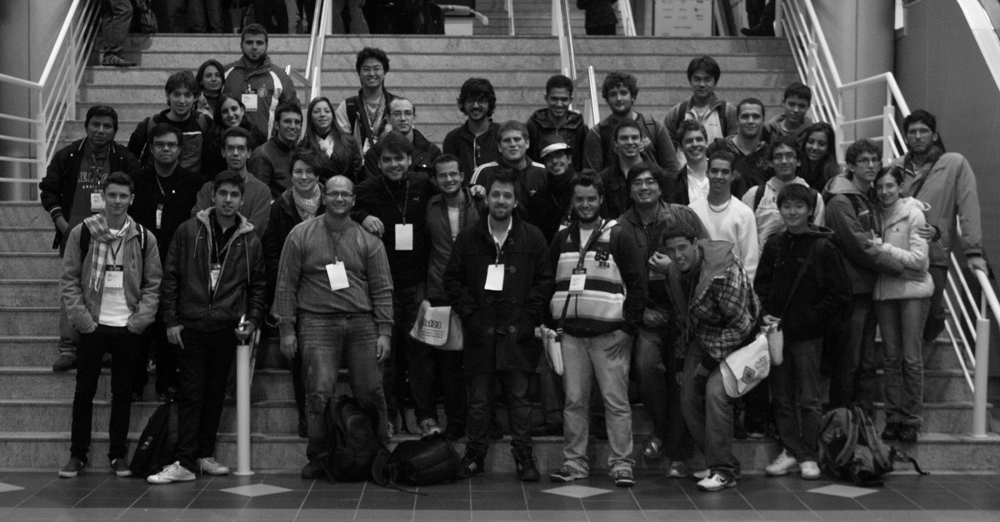
\includegraphics[width=.45\textwidth]{img/alem_da_graduacao/caco_fisl2.jpg}
\end{figure}

Participar do CACo é uma experiência diferente de tudo aquilo que você terá na
sua graduação. É a chance de aprender e crescer de uma forma que não acontece em
nenhuma aula de cálculo. É uma oportunidade de conhecer seus veteranos e também
seus amiguinhos bixos. Mas, acima de tudo, é uma experiência pessoal onde você
vai aprender a se expressar, argumentar, defender suas ideias, falar em público
e pensar no coletivo. Você entrará em contato com muita gente que provavelmente
você nunca iria conhecer e, com certeza, fará amizade com muitos deles. Por
esses e muitos outros motivos é que você, bixo, deve vir a pelo menos uma
reunião do CACo e sentir na pele tudo o que foi dito aqui. Venha nos ajudar a
fortalecer ainda mais o melhor CA da Unicamp. Até a reunião!

\begin{compactitemize}
    \item  E-mail: \email{caco@ic.unicamp.br}
    \item  Site: \url{www.caco.ic.unicamp.br}
    \item  Reuniões: você será informado no começo do semestre sobre os horários
        das reuniões. Participe!
\end{compactitemize}

Veja a seguir algumas das atividades que o CACo pratica:

\subsection{Avaliação de Curso e Reforma Curricular}

Uma vez por semestre, ocorre a reunião de avaliação de curso da qual participam
alunos, coordenadores e professores, além de responsáveis pela infraestrutura do
IC e da FEEC. Nela, são discutidos problemas relativos aos cursos, que vão desde
professores ruins até cadeiras quebradas. São avaliadas as disciplinas,
apontados problemas e indicadas soluções. A participação dos alunos é muito
importante, afinal somos nós que mais ganhamos e perdemos com o bom e o ruim de
nossos cursos. Por isso, o CACo participa dessa reunião levando a opinião dos
alunos para serem debatidas.

A avaliação de curso também visa a reforma curricular dos cursos. O catálogo do
curso (disciplinas que devem ser cursadas) é alterado todos os anos e a reunião
de avaliação tem grande papel nessas alterações.

\subsection{Caravana para o fisl}

O CACo organiza anualmente uma caravana para o fisl, o Fórum Internacional de
Software Livre, que acontece em Porto Alegre. O fisl reúne milhares de pessoas
de todo o mundo e conta com palestras e profissionais de renome. O Fórum é um
ótimo modo de entrar em contato com o mundo da computação e a caravana é uma
ótima e barata maneira de ir e tembém de socializar com outros computeiros.

\begin{figure}[H]
    \centering
    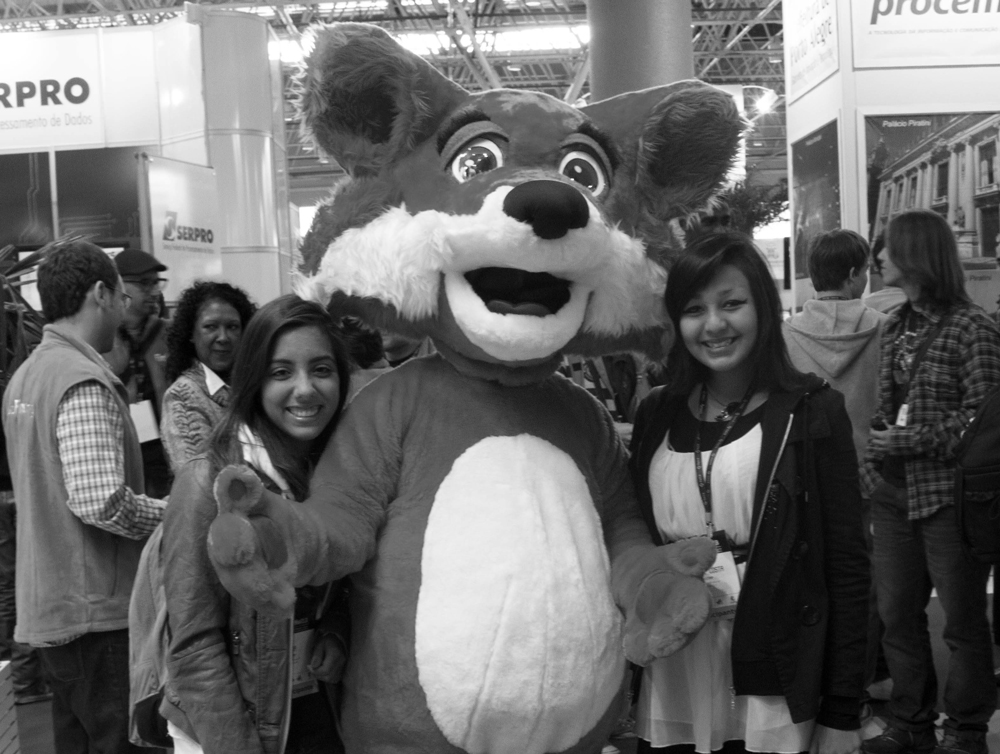
\includegraphics[width=.45\textwidth]{img/alem_da_graduacao/caco_fisl1.jpg}
\end{figure}

\subsection{Pesquisa Salarial}

Em 2010, com a colaboração do diretor do IC, o professor Hans Liesenberg, e da
rede social Reunion, promovemos uma pesquisa salarial com ex-alunos de
computação, que ajudou a fornecer um bom panorama da realidade em que se
encontra o profissional formado pela Unicamp na área de computação. A pesquisa
está disponível no site do CACo.

\subsection{CineCACo}

Por que não juntar com a galera no IC para assistir um filme com pipoca e
refriegerante de graça?

\subsection{PipoCACo}

Os PipoCACos são eventos de discussão sobre assuntos polêmicos, mas sem
comentários sobre  mamilos. Trata-se de um espaço para que toda a Computação
possa discutir um assunto de interesse geral. Por exemplo, já realizamos
PipoCACos sobre cotas em universidades públicas, sobre o Enade e semestralmente
fazemos o PipoCACo de Avaliação de Curso, onde reunimos as reclamações dos
alunos para a reunião de avaliação. Além de um ótimo local para ouvir opiniões e
debater, os PipoCACos são regados a refrigerante e pipoca por nossa conta!

\subsection{Palestra AA/AB}

Chega um momento na vida de todo computeiro engenheiro em que ele deve responder
às questões fundamentais como: De onde viemos? Para onde vamos? Onde vamos
almoçar hoje? Vou ser Azóide ou Bzóide?

O curso de Engenharia de Computação da Unicamp se divide em duas habilitações,
também conhecidas como modalidades: AA e AB. A diferença? Não é simples! Por
isso, o CACo organiza uma série de palestras a fim de ajudá-lo a escolher a
modalidade que mais lhe agrada.

\subsection{CACo Series of Poker}

O lendário torneio de Poker do CACo. Aberto a toda a computação, o CSoP é um
ótimo evento de integração e já contou com sete edições de absoluto sucesso!
Você será informado da data do próximo, fique ligado!

\begin{figure}[H]
    \centering
    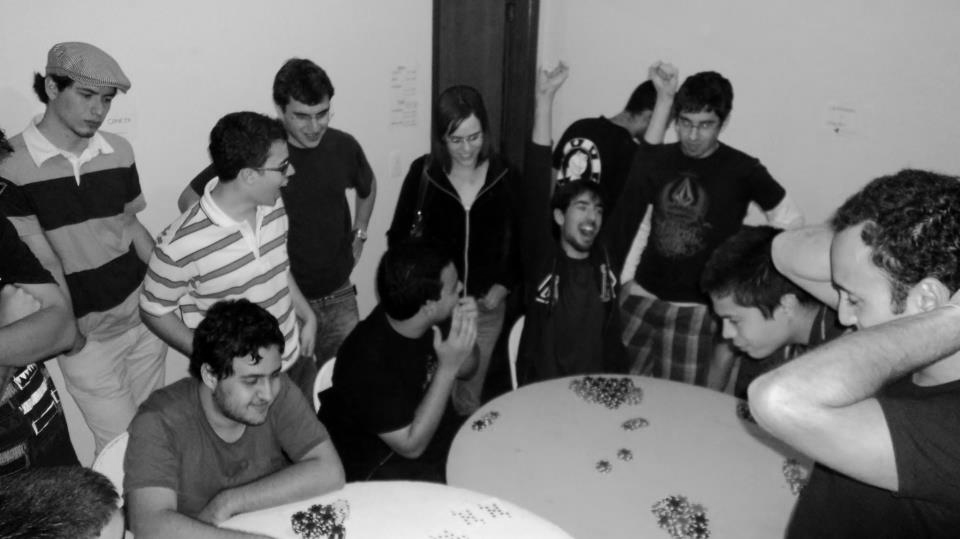
\includegraphics[width=.45\textwidth]{img/alem_da_graduacao/caco_poker2.jpg}
\end{figure}

\subsection{Salinha}

A sede do CACo fica na nossa salinha no IC-3. Munida de uma incrível mesa de
sinuca, ela está aberta 24/7 para todos os computeiros que queiram jogar.

\subsection{Atendimento}

O CACo realiza atendimentos na nossa salinha. Nesses horários, você poderá
comprar nossos produtos, se inscrever em algum de nossos eventos ou só bater
papo com a gente mesmo. Os horários de atendimento serão divulgados no início do
semestre e você pode conferi-los no site do CACo.

\begin{figure}[H]
    \centering
    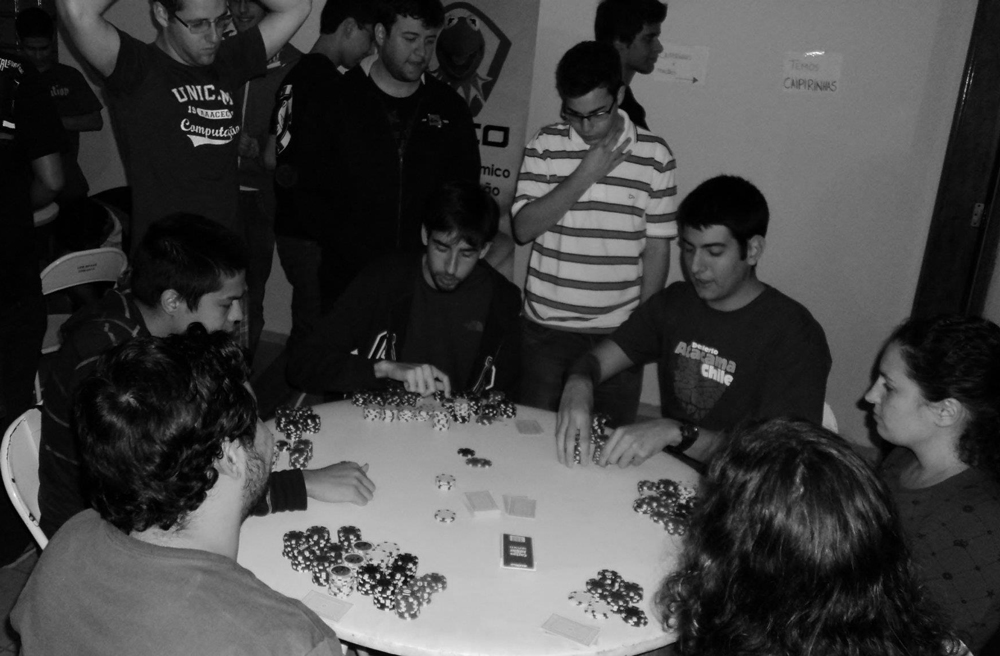
\includegraphics[width=.45\textwidth]{img/alem_da_graduacao/caco_poker1.jpg}
\end{figure}

\subsection{Manual do Bixo}

Esse excelente Manual que você está lendo agora não caiu do céu. Em tempos
imemoriais, o Manual do Bixo era feito pela Atlética, porém atualmente o CACo
assumiu a responsabilidade de editar, imprimir e distribuir o Manual aos
ingressantes todos os anos. Utilizamos Git pra controle de versão e {\LaTeX }
para formatação do conteúdo. Para contribuir, o melhor jeito é mandar pull
requests para nosso repositório, \url{github.com/cacounicamp/Manual-do-Bixo},
mas você também pode mandar um email pra gente com as contribuições caso você
não saiba usar Git ou \LaTeX.

\subsection{Gestão}

O CACo tem uma gestão composta de gente bonita e charmosa. Não se preocupe, se
você não é bonito nem charmoso, você ainda pode entrar na gestão... talvez. A
atual gestão foi eleita em novembro de 2014 e deve permanecer até outubro de
2015. Mas não pense que só a gestão gere o CACo. Mais uma vez: o CACo é o seu
centro acadêmico. Você e toda a computação também fazem parte do CACo e têm
papel nas nossas decisões e discussões.

Para ficar mais integrado ao que ocorre no seu centro acadêmico, como suas
ações, projetos e quais os problemas atuais, você pode se increver na lista do
CACo no Google Groups por meio do link:
\url{bit.ly/cacounicamp}.

\begin{figure}[H]
    \centering
    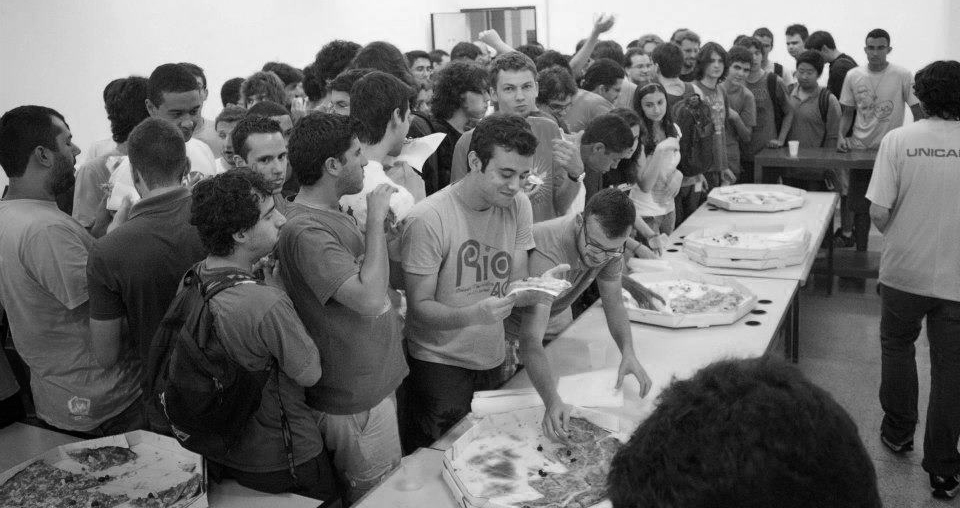
\includegraphics[width=.45\textwidth]{img/alem_da_graduacao/caco_pizzada2.jpg}
\end{figure}

\begin{figure}[H]
    \centering
    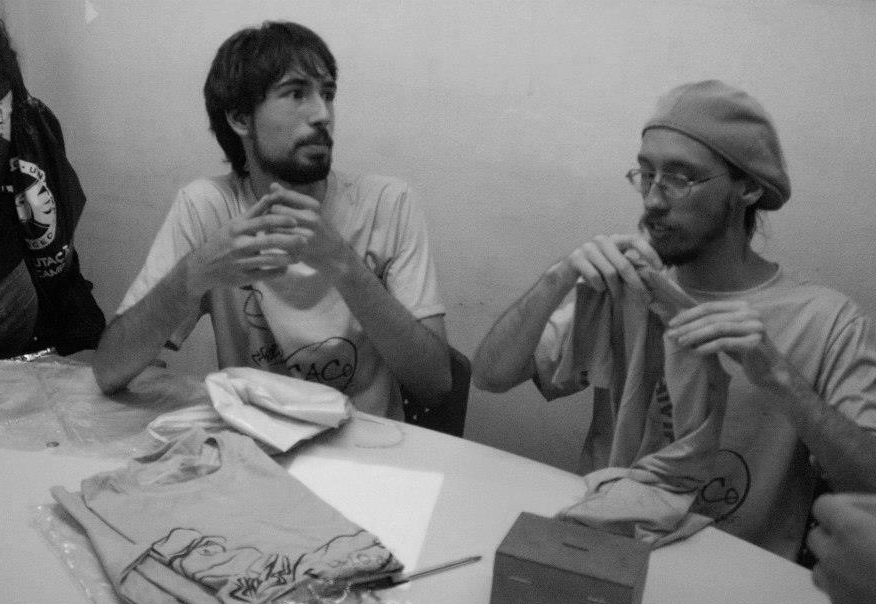
\includegraphics[width=.45\textwidth]{img/alem_da_graduacao/caco_eleicao.jpg}
\end{figure}

\subsubsection*{Chapa ``De Maior'' (2014/2015)}

\begin{itemize}
    \item   \textbf{Presidência}
        \\Lauro Cruz e Souza (Peta EC014)

    \item   \textbf{Coordenadoria Administrativa}
        \\Guilherme Lucas da Silva (Virose EC014)
        \\Henrique Noronha Facioli (Henrique EC014)

    \item   \textbf{Coodenadoria Financeira}
        \\Pedro Emílio Machado de Brito (Asmina EC012)
        \\Pedro Rodrigues Grijó (Grijó EC012)

    \item   \textbf{Coordenadoria de Ensino e Graduação}
        \\Gabriel Militão Vinhas Lopes (Gagau EC012)

    \item   \textbf{Coordenadoria de Comunicação e Marketing}
        \\Yuri Corrêa Pinto Soares (Yuri CC012)
        
    \item   \textbf{Coordenadoria de Eventos e Cultura}
        \\Isadora Sophia Garcia Rodopoulos (Isadora EC014)

    \item   \textbf{Coordenadoria de Produtos}
        \\Alex Wei (Boquinha EC014)

    \item    \textbf{Coordenadoria Tecnológica}
        \\Lucas Silva Schanner (Capivas EC014)
\end{itemize}

As gestões dos anos anteriores podem ser vistas no site do CACo.

\begin{figure}[H]
    \centering
    \includegraphics[width=.45\textwidth]{img/alem_da_graduacao/caco_pipocaco.jpg}
\end{figure}

\newpage
%%%%% Serviços da Unicamp
% Este arquivo .tex será incluído no arquivo .tex principal. Não é preciso
% declarar nenhum cabeçalho

\section{Serviços da Unicamp}
\subsection{Atendimento médico e odontológico -- CECOM}

A CSS é responsável pelo planejamento e execução de programas de saúde voltados
à comunidade universitária da Unicamp -- alunos, funcionários e docentes.  É
responsável também pelo atendimento à saúde oral desta comunidade, incluindo
também os filhos menores de servidores que estejam devidamente matriculados nas
creches e escolas dos campi.

Em português, isso quer dizer que é um ``plano de saúde'' da Unicamp. Demora um
pouco (embora o pronto-socorro do CECOM seja bem mais rápido que o do HC), tem
burocracia, mas funciona. Você pode marcar consultas médicas e fazer exames.  O
CECOM é localizado próximo ao HC. Para ir, é melhor pegar o Circular pois é
beeeeeem longe. De circular interno, peça para descer no CECOM. É o ponto final
ou o penúltimo dos circulares.

Fique de olho na sua caixa de entrada perto do período de inverno, pois o CECOM
costuma disponibilizar vacina contra gripe gratuitamente, uma dose em clínica
particular é bem cara, vale a pena.

Caso você tenha Unimed, o Centro Médico, que fica perto da Unicamp, atende pela
Unimed. É mais rápido que o atendimento da Unicamp (CECOM ou SUS).

%%% Imagem do hospital
\begin{figure}[h!]
    \centering
    \includegraphics[width=.45\textwidth]{img/alem_da_graduacao/hc.jpg}
    \caption{Vista do Hospital de Clínicas da Unicamp}
\end{figure}

Para marcar consultas com Dentista, vá ao CECOM e pergunte onde que é. Isso é
mais fácil que você tentar entender lendo aqui. Basicamente é embaixo do CECOM,
muito fácil de chegar se alguém apontar com e dedo e dizer ``ali''. Funciona
muito bem, o atendimento é ótimo. A única burocracia é assistir uma palestra
sobre doenças da boca e escovação antes de poder marcar atendimento. Mas se você
estiver com dores eles te atendem na hora sem marcar consulta nem assistir
palestra.

Para saber mais sobre o CECOM, vá ao site deles (\url{www.cecom.unicamp.br}).

\subsection{Hemocentro}

Essa é para quem é (ou para quem quer ser) doador de sangue. O centro de
hematologia e hemoterapia (Hemocentro) é o órgão da Unicamp responsável pela
coleta e doação de sangue.
\begin{wrapfigure}{r}{.2\textwidth}
    \centering
    \includegraphics[width=.2\textwidth]{img/alem_da_graduacao/doe_sangue.jpg}
\end{wrapfigure}
Qualquer pessoa pode aparecer no Hemocentro para fazer a doação de sangue. Basta
estar com o RG e seguir um conjunto de normas para a doação de sangue. Para
saber mais sobre o processo, é só visitar a página do Hemocentro
(\url{www.hemocentro.unicamp.br}).

O Hemocentro também faz o projeto doador universitário, que consiste de unidades
móveis (ônibus) que param em alguns pontos do campus. Essas unidades fazem a
coleta do sangue. Alunos, professores e funcionários podem ir até essas unidades
móveis para fazer a doação. Para se informar melhor, é só visitar a página do
projeto: \url{bit.ly/14xaTAn}.

O Hemocentro fica localizado acima do HC (próxima ao CECOM). Portanto, se quiser
se deslocar até lá, como está escrito acima, é melhor usar o circular interno.

\subsection{Circular Interno e Ônibus Moradia}

\subsubsection{Circular Interno}
É um serviço de ônibus gratuito que dá voltas na Unicamp. Há duas linhas, uma
girando no sentido horário e outra no anti-horário.  Só funciona até às 19h, e a
frequência maior é no horário de almoço. Bom para cobrir percursos como bandejão
ao IC, IC à FEEC, qualquer lugar ao CECOM, qualquer lugar à FEAGRI, FEAGRI à
qualquer lugar. Quase todos os pontos têm os itinerários e os horários afixados.
Ele não costuma atrasar nem adiantar mais que 5 minutos, exceto no período de
férias.

\subsubsection{Circular Noturno}
É um ônibus que dá uma volta na Unicamp partindo do balão da Avenida 1, passando
pela BC, IQ, FEEC, IC e voltando para o balão da Avenida 1.  Os horários e o
itinerário desse ônibus não estão nos pontos como os do Circular Interno 1 e do
2. Ele funciona das 19h às 23h, a cada meia hora.

\subsubsection{Ônibus Moradia}
Também conhecido como ``Circular Externo'', dá uma volta na Unicamp partindo da
BC, vai para a Moradia e faz o caminho contrário. Ele também tem duas rotas
alternativas em horários específicos que cobrem as regiões da Avenida 1, Centro
de Barão Geraldo e Avenida 3. Os horários mais lotados do Ônibus Moradia são 8
da manhã (sentido Moradia--Unicamp), horário de almoço (ambos os sentidos),
horário de jantar (ambos os sentidos) e o último horário (Unicamp--Moradia). Se
puder evitar esses horários, faça-o.

Todos os itinerários e horários detalhados dos serviços de ônibus podem ser
encontrados na página da Prefeitura da Unicamp: \\\url{prefeitura.unicamp.br}.
Você também consegue acessá-los a partir do aplicativo Unicamp Serviços,
disponível pra Android e iOS.

\subsection{SAE -- Serviço de Apoio ao Estudante}
\begin{wrapfigure}{l}{.2\textwidth}
%\begin{figure}[h!]
    \centering
    \includegraphics[width=.2\textwidth]{img/alem_da_graduacao/sae.jpg}
%\end{figure}
\end{wrapfigure}
O SAE (Serviço de Apoio ao Estudante), principal órgão de apoio ao estudante na
Unicamp, atua em várias frentes de assistência estudantil. Esta se dá por meio do
gerenciamento de bolsas-auxílio, assistência social e orientações educacional,
jurídica e psicológica, além de apoio a projetos acadêmicos e sociais e programa
de intercâmbio de estudantes no exterior. O SAE também é responsável pela gestão
de estágios na Universidade.

\begin{itemize}
    \item  Localização: Prédio do Ciclo Básico, 3º piso (responsável pelo
        gerenciamento de convênios, estágios, bolsa-pesquisa e bolsa-empresa); e
        ao lado da cantina do DCE (serviço social, responsável pelo gerenciamento 
        de\\ bolsas-auxílio).
    \item  Horário: Segunda a sexta, das 08h30 às 20h, no período letivo.
    \item  Contato: \email{sae@unicamp.br}
    \item  Site: \url{www.sae.unicamp.br}
\end{itemize}

\subsection{Bolsas-Auxílio}
\subsubsection{Moradia}

Criado em 1989, o Conjunto Residencial Universitário da Unicamp, tem por
finalidade garantir estadia gratuita e de qualidade para os estudantes que
passam por dificuldades sócio-econômicas.

Para saber mais sobre o processo seletivo entre no site da Moradia da Unicamp
(\url{www.pme.unicamp.br}).

\subsubsection{Bolsa Alimentação e Transporte}

Objetivo: Colaborar com o estudante de graduação e pós-graduação em dificuldade
sócio-econômica, nos itens alimentação e transporte.

Critérios para a seleção: Análise do questionário sócio-econômico devidamente
preenchido e documentado, e entrevista com a assistente social.

\subsubsection{Bolsa Trabalho}

Objetivo: Colaborar com o estudante de graduação em dificuldade sócio-econômica,
cuja família não tenha condições de mantê-lo na Universidade. Em contrapartida o
bolsista trabalhará 15 horas semanais em unidades da Unicamp, ou em grupos de
pesquisas, ou em grupos sociais, em horário compatível com o horário escolar.  E
com a orientação de um professor.

Critérios para a seleção: Análise do questionário sócio-econômico devidamente
preenchido e documentado, e entrevista com a assistente social.

Alunos da pós não podem se candidatar à bolsa trabalho.

\subsubsection{Bolsa Emergência}

Objetivo: Atender os estudantes de graduação regularmente matriculados que
estejam passando por dificuldades econômicas emergenciais. Em contrapartida o
bolsista trabalhará 40 horas em unidades da Unicamp, compatível com o horário
escolar.

Procedimento: o candidato deverá enviar uma carta à Coordenação do SAE
solicitando o benefício e informando sobre os motivos. Preencher e entregar
devidamente documentado o questionário sócio-econômico e marcar entrevista com a
assistente social.

Critérios para seleção: Análise da solicitação, do questionário sócio-econômico
devidamente preenchido, documentado e entrevista com a assistente social.

Alunos da pós não podem se candidatar à bolsa emergência.

\subsubsection{Bolsa PAPI}

Busca incentivar a participação de alunos de graduação e de pós-graduação nas
mais diversas atividades da Unicamp, tais como no auxílio a eventos. Neste
programa, há a solicitação de estudantes por parte de alguma Unidade ou órgão da
Unicamp, que poderá indicar o nome do aluno ou deixar a critério do SAE para
fazê-lo.

\subsection{Assistência Jurídica}

Objetivo: Orientar os alunos nacionais ou estrangeiros de graduação ou
pós-graduação, na resolução de suas questões pessoais de cunho jurídico que
envolvam os ramos do Direito, principalmente os seguintes:

\begin{description}
    \item[Direito Civil:] Contratos em geral; contratos de locação de
        imóvel/escritura de compromisso de venda e compra; acidentes de
        trânsito; reparação de dano; ação revisional de aluguel; separação
        judicial; divórcio; pensão alimentícia, etc.

    \item[Direito Penal:] Violência contra a pessoa; lesões corporais; furto;
        roubo etc{\dots}

    \item[Direito do Trabalho:] Caracterização de relação de emprego para os não
        registrados e direitos trabalhistas em geral (Normas da CLT).
\end{description}

Procedimento: O aluno deve dirigir-se pessoalmente ao SAE para obter os
esclarecimentos desejados.

Delitos de consumo, encaminhar ao SEDECON ou ao PROCON.

Com relação aos contratos de locação alertamos para algumas dicas importantes:

\begin{itemize}
    \item  Jamais pagar qualquer valor antecipadamente (ex: ``taxas de reserva
        de imóvel'', ``taxa de contrato'', aluguel antecipado etc), ou fornecer
        títulos em garantia: (cheque pré-datado, nota promissória).

    \item  Obter o maior número de informações possíveis relativas ao imóvel,
        proprietário(s), imobiliária, procuradores;

    \item  Condições e valores para pagamento (aluguel e outros encargos ex.:
        Condomínio, IPTU, seguros etc, para uma real visualização do valor total
        a ser despendido).

    \item  Sempre solicitar uma Minuta do contrato locação.

    \item  Não assinar contrato ou qualquer outro documento antes de
        apresentá-lo para análise por um dos advogados da O.J. SAE.
\end{itemize}

\subsection{Orientação psicológica}

Objetivo: Prestar atendimento psicológico ao aluno de graduação, pós-graduação e
especial.

O Serviço de Orientação Psicológica do SAE funciona em associação com o Serviço
de Atendimento Psicológico e Psiquiátrico ao Estudante (SAPPE) do Departamento
de Psicologia Médica e Psiquiatria da FCM, desde a sua implantação, em 1987.

Funcionamento e informações:

\begin{itemize}
    \item  Existem horários para consultas imediatas (ideais para quem está
        prestes a expulsar um amigo da república etc);

    \item  O tratamento de longo prazo é obtido mediante uma palestra
        explicativa, um horário de atendimento individual e espera em uma lista
        de candidatos -- horários disponíveis e motivos especiais podem
        facilitar seu ingresso, mas lembre-se: não é porque aparentemente não
        parece importante o motivo pelo qual você procura ajuda que isso não
        deva ser levado a sério. Em alguns casos, apenas quatro seções são
        suficientes para a pessoa sair do tratamento (lembrando que ele pode ser
        interrompido a qualquer momento);

    \item  Há possibilidade de tratamento em grupo terapêutico, psicoterapia
        individual, de família e de casal com uma das psicólogas da equipe. O
        grupo terapêutico é formado levando-se em conta que não devem haver
        pessoas muito próximas em sua formação, como condição de que o paciente
        tenha liberdade para falar de seus problemas com menos receio.
\end{itemize}

\subsection{Cadastro de veículos}

Para você poder entrar e sair da Unicamp sem ter de parar para receber e
entregar o papel de identificação do veículo você pode cadastrar seu carro junto
à Prefeitura do Campus. O cadastramento do veículo deverá ser feito diretamente
na Central de Informações (próximo ao Balão da avenida 1) de segunda a
sexta-feira das 09h às 17h.

Documentos necessários:

\begin{itemize}
    \item  Identidade funcional (para funcionários e docentes), identidade
        estudantil para alunos, carta de apresentação da unidade para
        estagiários;
    \item  Documento do veículo;
    \item  Preenchimento de declaração.
\end{itemize}
Há possibilidade de se cadastrar até três veículos, com um custo de R\$ 5,00
para o segundo e de R\$ 10,00 para o terceiro veículo.

\subsection{Licenças de Software Gratuitas}

Bixo, agora que você é um computeiro de verdade, sua responsabilidade de não
usar software pirata é ainda maior. Afinal de contas, em poucos anos você pode
estar do lado dos desenvolvedores -- e não apenas consumidores -- de software.

A vantagem é que, por estar na Unicamp, você agora tem acesso a várias licenças
gratuitas de software proprietário especiais para estudantes.

O LMS (Laboratório Microsoft) ligado ao Instituto de Computação oferece download
gratuito de uma grande variedade de software da Microsoft, como o sistema
\textbf{Windows} e o ambiente de desenvolvimento integrado (leia-se: serve para
programar) \textbf{Visual Studio}. O Office não está disponível. Para mais
informações sobre como se cadastrar e baixar, acesse:
\url{www.lms.ic.unicamp.br}.

A CTIC (Coordenadoria de Tecnologia da Informação e Comunicação) obtém licenças
de muitos pacotes de software e disponibiliza para a comunidade acadêmica,
inclusive alunos. As aplicações de computação científica \textbf{Wolfram
Mathematica} e \textbf{MATLAB} estão disponíveis gratuitamente. Para mais
informações, acesse: \url{www.ctic.unicamp.br/softwares}.

A multinacional Autodesk oferece licenças de estudante gratuitas para muitos de
seus programas, incluindo o \textbf{AutoCAD} e a aplicação de modelagem 3D
\textbf{Maya}. Para baixar, cadastre-se usando seu e-mail da DAC, do IC ou da
FEEC em \url{students.autodesk.com}.

\subsection{Jornal da Unicamp}

O jornal da Unicamp é um jornal de distribuição semanal distribuído dentro da
Unicamp. Podem-se encontrar diversos exemplares do jornal na sala de
computadores que fica ao lado da DAC, no IC-2 e em diversos pontos espalhados
pelo campus.

No jornal são mostradas as diversas pesquisas realizadas pela universidade,
eventos, livros e obras de autoria de professores, aparições da Unicamp na
imprensa e defesas de mestrado e doutorado.

Na página do jornal (\url{www.unicamp.br/ju}) podem-se encontrar as últimas
edições do jornal (em PDF), além de poder fazer a assinatura online do jornal,
distribuído em formato PDF. A assinatura e distribuição do jornal são gratuitas.

\newpage
%%%%% Jornal da Unicamp
% Este arquivo .tex será incluído no arquivo .tex principal. Não é preciso
% declarar nenhum cabeçalho

\section{Jornal da Unicamp}

O jornal da Unicamp é um jornal de distribuição semanal distribuído dentro da
Unicamp. Podem-se encontrar diversos exemplares do jornal na sala de
computadores que fica ao lado da DAC, no IC-2 e em diversos pontos espalhados
pelo campus.

No jornal são mostradas as diversas pesquisas realizadas pela universidade,
eventos, livros e obras de autoria de professores, aparições da Unicamp na
imprensa e defesas de mestrado e doutorado.

Na página do jornal (\url{www.unicamp.br/ju}) podem-se encontrar as últimas
edições do jornal (em PDF), além de poder fazer a assinatura online do jornal,
distribuído em formato PDF. A assinatura e distribuição do jornal são gratuitas.

\newpage
%%%%% Eventos da Unicamp
% Este arquivo .tex será incluído no arquivo .tex principal. Não é preciso
% declarar nenhum cabeçalho

\section{Eventos da Unicamp}
\subsection{Feira do Livro}

Evento iniciado em 2002, a cada dois anos a Editora da Unicamp realiza a Feira
do Livro, no Ginásio da Unicamp. Há excelentes opções, de diversas editoras,
principalmente na área de literatura, artes e humanas, com no mínimo 50\% de
desconto.

\subsection{Semanas da Unicamp}

Alguns cursos da Unicamp realizam anualmente um evento (chamado de Semana) em
que os alunos de graduação têm um contato com o mercado de trabalho, com as
pesquisas, com as tendências e novidades dos cursos e demais assuntos, ramos e
áreas de cada curso. Para isso, participam desse evento ex-alunos e
profissionais, realizam-se palestras e minicursos, são feitas visitas a empresas
e são feitos debates (mesas redondas).

\subsubsection*{Secomp -- Semana da Computação}

\begin{figure}[H]
    \centering
    \includegraphics[width=.35\textwidth]{img/alem_da_graduacao/secomp_logo.png}
\end{figure}

A Computação tem a sua própria semana, organizada por três entidades estudantis:
CACo, AAACEC e Conpec. O evento busca aproximar e relacionar os três pilares da
graduação: os alunos, a universidade e o mercado. Dessa forma, a Secomp --
Semana da Computação -- procura mostrar aos alunos a diversidade de caminhos a
seguir e um pouco do que cada área pode oferecer.

Durante seus sete dias de duração, a Semana traz uma gama de atividades, entre
palestras, oficinas, cursos, visitações e outros eventos, para que os
participantes possam ter uma visão abrangente do mercado e da própria
universidade. Além disso, a Secomp tem atividades voltadas ao recrutamento em
grandes empresas, para aqueles à procura de vagas.

Se você acha que nada disso importa, bixo, você é burro, mas não tem problema.
A Semana também tem uma fartura -- literalmente -- de coffee-breaks, brindes e
prêmios sorteados. Tudo isso por um preço simbólico, menor do que o de uma
balada no Campinas Hall. Não perca!

\subsection{Talento}

Talento é um evento que acontece todo ano, desde 1999, durante um dia inteiro,
no Ginásio Multidisciplinar e organizado pelo Núcleo de Empresas Juniores da
Unicamp. Trata-se de uma feira de recrutamento, onde alunos da Unicamp e de
outras universidades e o público em geral têm contato com empresas, seja por
meio de palestras, mesas redondas e estandes, e estas apresentam o seu processo
seletivo. Nesse evento também é feito o cadastro de currículos dos visitantes.

Para saber mais sobre o evento, é só acessar a página da Talento
(\url{talentounicamp.com.br}). O evento é gratuito.

\subsection{UPA -- Unicamp de Portas Abertas}

\begin{figure}[h!]
    \centering
    \includegraphics[width=.45\textwidth]{img/alem_da_graduacao/bateria_upa.jpg}
\end{figure}

A \textbf{UPA} é um evento anual em que, durante um dia, geralmente no mês de
setembro, a Unicamp é apresentada para estudantes dos ensinos fundamental e
médio de todo o país, muitos dos quais pré-vestibulandos. A apresentação da
universidade é feita por professores e alunos, que mostram as salas de aula e as
pesquisas realizadas.

No ano de 2013, a UPA recebeu a visita de 40 mil alunos de 639 escolas públicas
e privadas, originárias de vários estados do Brasil.

O IC costuma realizar uma recepção com forte participação dos alunos. Se você é
como todo bixo e está louco para pagar de estudante da Unicamp, esta é uma
oportunidade excelente! Além de ser divertido, o IC geralmente oferece uma
pequena remuneração pelo trabalho. Participe!

Para saber mais sobre o evento, é só acessar a página \url{www.upa.unicamp.br}.

\newpage
%%%%% Agora eu tenho um e-mail da Unicamp
% Este arquivo .tex será incluído no arquivo .tex principal. Não é preciso
% declarar nenhum cabeçalho

\section{Agora eu tenho um e-mail da Unicamp}

Ao ingressar num curso de computação, você recebe pelo menos duas contas de
e-mail: do IC e da DAC. Estes são os principais meios de comunicação da
Universidade com você, portanto fique esperto e não deixe de ler esses emails
regularmente!

Para acessar o webmail do IC, o endereço é \url{webmail.students.ic.unicamp.br}.
O usuário e a senha são os mesmos do sistema Linux do IC, que você receberá nas
primeiras semanas de aula. Caso tenha dúvidas, dê uma passada na Secretaria de
Graduação, que fica no IC-2 (prédio ao lado das Artes Cênicas e para cima da
Economia) e pergunte!

Uma dica interessante, que muitas vezes passa despercebida, é que no mesmo
documento em que você recebe sua senha, vem indicado um {\it alias} para o seu
e-mail. Assim, você poderá utlizá-lo de uma forma mais amigável, ao invés de ser
somente o seu próprio RA, por exemplo:

\begin{center}
\texttt{francisco.silva@students.ic.unicamp.br}\\
em vez de\\
\texttt{ra129873@students.ic.unicamp.br}
\end{center}

A DAC também dispõe um webmail para o aluno. O login é a primeira letra do nome
do aluno, seguido dos dígitos do RA. O e-mail da DAC também é útil. É nele que
os alunos são avisados sobre o período de matrícula, recebem os seus pedidos de
matrículas provisórias, avisos de desistências e trancamentos, além de informar
os alunos a respeito de eventos que acontecem na Unicamp, como feiras,
palestras, festivais, eleições. O endereço do webmail da DAC é
\url{webmail.dac.unicamp.br}.

Para a galera da Engenharia, ainda há o e-mail da FEEC, que muitos sequer ficam
sabendo que existe! Só um semestre ou até um ano depois vão até o SIFEEC retirar
seu login e senha. Ou então ficam sabendo só no segundo ou terceiro ano de curso
e aí há mais de 700 e-mails não lidos. Assim como o do IC, é muito utilizado
para divulgação de eventos, oportunidades de estágios e de iniciação científica.
Para utilizá-lo, você deve ir até a FEEC e procurar o SIFEEC, que é o local
responsável por isso. Fica no segundo andar do prédio de laboratórios da FEEC
(um com escadas amarelas). O endereço do webmail da FEEC é
\url{webmail.fee.unicamp.br} e a senha é a mesma do Linux da FEEC.

\begin{figure}[b!]
    \centering
    \includegraphics[width=.3\textwidth]{img/alem_da_graduacao/email.jpg}
\end{figure}
Você também pode redirecionar os e-mails que receber nas contas do IC, FEEC e
DAC para qualquer outra conta (no Gmail por exemplo).

\subsection{Redirecionamento de e-mails}
Para efetuar o redirecionamento do e-mail institucional para outro e-mail, siga
os passos abaixo para cada e-mail institucional que você tiver.

\subsubsection*{E-mail da DAC}

\begin{compactenumerate}
    \item  Acesse \url{www.dac.unicamp.br}
    \item  Acesse Serviços On-line
    \item  Acesse Alunos
    \item  Clique em Acesso aos Serviços Acadêmicos
    \item  Faça login
    \item  Clique em Redirecionamento de Email
\end{compactenumerate}

\subsubsection*{E-mail da FEEC}

\begin{compactenumerate}
    \item  Acesse \url{webmail.fee.unicamp.br}
    \item  Faça login
    \item  Acesse Options
    \item  Acesse Mail Forwarding
\end{compactenumerate}

\subsubsection*{E-mail do IC}

\begin{compactenumerate}
    \item  Acesse \url{webmail.students.ic.unicamp.br}
    \item  Faça login
    \item  Acesse Filtros
    \item  Clique em Adicionar uma nova regra
    \item  Em Condição, na primeira lista drop-down com a opção Header, escolha a opção All
    \item  Em Ação, escolha Redirecionar para o seguinte endereço de e-mail
\end{compactenumerate}

\subsection{Tenha uma conta no Gmail!}

Nós sabemos que é difícil. Muitas vezes você vem usando um serviço de e-mail
durante anos, seja ele Hotmail, Yahoo, Uol, Terra, Zipmail, e mudar é
trabalhoso.  Mas confie na gente: agora vai ser mais fácil. Você está começando
uma vida nova na universidade, quando já tiver cadastrado seu endereço antigo em
vários serviços acadêmicos e divulgado entre os novos contatos que vai fazer,
será bem mais complicado.

Entre as vantagens do Gmail, podemos destacar:

\begin{itemize}
    \item Muito espaço, nunca mais apague nada.
    \item Visualização em threads, útil para acompanhar discussões.
    \item Bom aplicativo para smartphones.
    \item Filtros e marcadores infinitos para te ajudar.
    \item Uma pesquisa que funciona.
    \item Interface mais polida que as da concorrência.
\end{itemize}

Qualquer dúvida, novamente, procure um veterano!

Finalizando, não deixe de estar sempre informado sobre os acontecimentos ou
divulgações da Unicamp, do CACo, da AAACEC e da Conpec, essas três entidades
compostas por alunos de computação.


\end{document}
